\documentclass[10pt]{article}

%% Packages
\usepackage[margin=1in, top=0.75in]{geometry}
\usepackage[utf8]{inputenc}
\usepackage[T1]{fontenc}
\usepackage[usenames,dvipsnames]{xcolor}
\usepackage{amssymb, amsfonts, amsmath, mathrsfs, enumitem, tcolorbox, bbm, graphicx, fullpage, parskip, mathtools, float, amsthm}
\usepackage{tikz,sgame,bbm,todonotes, setspace, soul, array}
\usepackage[english]{babel}
\usepackage{pdfpages}
\setcounter{tocdepth}{3}
% Links (and references)
\definecolor{linkblue}{RGB}{40, 50, 200}
\usepackage[colorlinks=true, allcolors={linkblue}]{hyperref}

%% Math operators
\newcommand*{\ones}{\text{\usefont{U}{bbold}{m}{n}1}}
\newcommand{\reals}{\mathbb{R}}
\newcommand{\rationals}{\mathbb{Q}}
\newcommand{\integers}{\mathbb{Z}}
\newcommand{\naturals}{\mathbb{N}}
\newcommand{\complex}{\mathbb{C}}
\newcommand{\normal}{\mathcal{N}}

% General math
\newcommand{\abs}[1]{\mathop{\left|#1\right|}} % absolute value
\newcommand{\inv}{^{-1}} % inverse
\let\oldST\st
\newcommand{\strikethrough}{\oldST}
\renewcommand{\st}{\;\text{s.t.}\;} % math operator for "such that"
\newcommand{\eg}{\emph{e.g.} }
\newcommand{\ie}{\emph{i.e.} }
\newcommand{\interior}{\mathop{\rm int}}

% Optimization
\newcommand{\argmax}{\mathop{\rm argmax}}
\newcommand{\argmin}{\mathop{\rm argmin}}
\newcommand{\opt}{^\star}
% Analysis, vector spaces, and topology
\newcommand{\set}[1]{\left\{#1\right\}} % set notation
\newcommand{\seq}[1]{_{#1}^{\infty}} % add sequence notiation to set (or to a summation symbol for series)
\newcommand{\setless}{\mathop{\backslash}} % A \ B notation
\newcommand{\pow}{\mathop{\mathcal{P}}} % power set
\newcommand{\im}{\mathop{\rm im}} % image
\newcommand{\spans}{\mathop{\rm span}} % span
\newcommand{\rank}{\mathop{\rm rank}} % rank
\newcommand{\topo}{\mathop{\mathcal{T}}} % topology
\newcommand{\cont}{\mathop{\bf C}} % continuously differentiable

% Matrices
\newcommand\colvector[1]{\begin{bmatrix}#1\end{bmatrix}}
\newcommand\rowvector[1]{\begin{bmatrix}#1\end{bmatrix}}
\newcommand\matrixc[1]{\begin{bmatrix}#1\end{bmatrix}}
\newcommand\matrixp[1]{\begin{pmatrix}#1\end{pmatrix}}
\newcommand\detmatrix[1]{\begin{vmatrix}#1\end{vmatrix}}
\newcommand\rankmatrix{\begin{bmatrix}I_r & \rvline & \mathbf{0}_1\\\hline \mathbf{0}_2 & \rvline & \mathbf{0}_3 \end{bmatrix}}

% Statistics
\newcommand{\cov}{\mathop{\rm cov}} % covariance
\newcommand{\corr}{\mathop{\rm corr}} % correlation
\newcommand{\expect}{\mathop{\mathbb{E}}} % expectation
\newcommand{\indep}{\perp \hspace{-1.4ex} \perp} % independence symbol
\newcommand{\distiid}{\mathop{\overset{\text{i.i.d.}}\sim}} % i.i.d.
\newcommand{\oversim}[1]{\mathop{\overset{\text{#1}}\sim}} % general text over \sim
\newcommand{\prob}{\mathbb{P}}
\newcommand{\mse}{\mathop{\rm MSE}}
\newcommand{\var}{\mathop{\rm Var}}
\newcommand{\sd}{\mathop{\rm sd}}
\newcommand{\se}{\mathop{\rm se}}
\newcommand{\bias}{\mathop{\rm bias}}
\newcommand{\toprob}{\overset{p}{\to}}
\newcommand{\toas}{\overset{a.s.}{\to}}
\newcommand{\todist}{\overset{d}{\to}}
\newcommand{\hyp}{\mathbb{H}}

% Economics
\newcommand{\choice}{\mathop{C_{\succsim}}} % choice correspondence

% Update existing operators
\let\oldExists\exists
\renewcommand{\exists}{\oldExists\;}
\let\oldForall\forall
\renewcommand{\forall}{\;\oldForall\;}
\let\oldEmptyset\emptyset
\renewcommand{\emptyset}{\mathop{\varnothing}}
\newcommand{\parl}{\left(}
\newcommand{\parr}{\right)}
\newcommand{\midbar}{\middle|}
\newcommand{\barl}{\left[}
\newcommand{\barr}{\right]}
\newcommand{\curll}{\left\{}
\newcommand{\curlr}{\right\}}


%% Presentation environments
% Proofs, counterexamples, and disproofs
\renewcommand\qedsymbol{$\openbox$}
\renewenvironment{proof}{{\raggedright \textit{\textbf{Proof.}}}}{\qed} % Proof
\newenvironment{pf}{\begin{proof}}{\end{proof}} % Proof (shorthand)

\newenvironment{disproof}{{\raggedright \textit{\textbf{Disproof.}}}}{$\qed$} % Disproof
\newenvironment{counterex}{{\raggedright \textit{\textbf{Counterexample.}}}}{} % Counterexample

% Theorem styles
\theoremstyle{plain}
\newtheorem{result}{Result}
\newtheorem{lemma}{Lemma}[section]

\newtheorem{theorem}{Theorem}[section]
\newtheorem{proposition}{Proposition}[section]
\newtheorem{corollary}{Corollary}[section]
\newtheorem{axiom}{Axiom}[section]
\theoremstyle{definition}
\newtheorem*{example}{Example}
\newtheorem*{definition}{Definition}
\newtheorem*{exercise}{Exercise}
\newtheorem*{model}{Model}
\newtheorem*{proposition*}{Proposition}
\newtheorem*{model*}{Model}
\newtheorem*{solution}{Solution}
\newtheorem*{remark}{Remark}
\newtheorem*{question}{Question}
\newtheorem*{answer}{Answer}
\newtheorem*{algorithm}{Algorithm}
\newtheorem{assumption}{Assumption}[section]

\newcommand{\blue}[1]{\textcolor{blue}{\emph{#1}}}
\newcommand{\red}[1]{\textcolor{red}{\emph{#1}}}




\newcommand{\gabe}[1]{\todo[inline,color=green!20!white]{\textbf{GS:} #1}}


%% Header
\makeatletter
\newcommand{\course}[1]{\def\@course{#1}}
\newcommand{\term}[1]{\def\@term{#1}}
\renewcommand{\title}[1]{\def\@entitle{#1}}
\renewcommand{\maketitle}{
    \begin{tcolorbox}[colframe=darkgray]
        \begin{center}
            \textbf{\@course} \\[0.25em]
            {\Large\textit{\@entitle}} \\[0.5em]
            \@author \\[0.5em]
            \@term
        \end{center}
    \end{tcolorbox}
    \vspace{1em}
}
\makeatother


%% Code
\usepackage{listings}
\usepackage{beramono}
\lstdefinelanguage{Julia}%
  {morekeywords={abstract,break,case,catch,const,continue,do,else,elseif,%
      end,export,false,for,function,immutable,import,importall,if,in,%
      macro,module,otherwise,quote,return,switch,true,try,type,typealias,%
      using,while},%
   sensitive=true,%
   alsoother={$},%
   morecomment=[l]\#,%
   morecomment=[n]{\#=}{=\#},%
   morestring=[s]{"}{"},%
   morestring=[m]{'}{'},%
   breaklines=true,%
}[keywords,comments,strings]%

\lstset{%
    language         = Julia,
    basicstyle       = \ttfamily,
    keywordstyle     = \bfseries\color{blue},
    stringstyle      = \color{magenta},
    commentstyle     = \color{ForestGreen},
    showstringspaces = false,
}






\title{Econometrics Notes}
\author{Gabe Sekeres}
\course{ECON 6200}
\term{Spring 2025}

\singlespacing

\begin{document}
\maketitle

\tableofcontents
\newpage


\section*{Introduction}

This course builds directly on ECON 6190, \href{https://gabesekeres.com/resources/private/fall_2024/econ_6190_notes.pdf}{the material} will not be revised. If you need to catch up on the material, especially probability and statistics, see the \href{https://users.ssc.wisc.edu/~bhansen/econometrics/}{Hansen} and \href{https://services.math.duke.edu/~rtd/PTE/PTE5_011119.pdf}{Durrett} textbooks. If there's one econometrics book to actually own, it's the Hansen. These notes will often reference results in either Hansen or \href{https://press.princeton.edu/books/hardcover/9780691010182/econometrics}{Hayashi}.

 See the syllabus for how we will be assessed -- homework is 30\%, prelim is 30\%, and the final is 40\%. For homework, you are invited (and \emph{highly} recommended) to form study groups! It's completely okay to work on the homeworks in study groups, but you will submit individual write-ups.

Roughly, in the first few weeks, we will start with the linear model in some detail. We will then generalize to IV, TSLS, and go rapidly to the Generalized Method of Moments (GMM) and extremum (or $m$-) estimation. We will also cover some nonparametrics as well as bootstrap.

You can think of us starting in the most specific case and moving outwards. OLS is a special case of IV, which is a special case of TSLS, which is a special case of GMM, which is a special case of extremum estimation. We will also think about Maximum Likelihood (ML) as a special case of extremum estimation, and panel data as a special case of GMM. Studying this tree will cover half of the course, and then we will have some time to cover nonparametric methods like kernel density and kernel mean, as well as bootstrapping. This may seem like we are doing some old school stuff, since the other ML (machine learning) has overtaken these methods, but theoretically they are very similar.

\section{The Linear Model}

We have, of course, already encountered the 

\begin{definition}
	\blue{Ordinary Least Squares (OLS)} estimator:
	\begin{align*}
		\hat{\beta} &= \parl X' X\parr^{-1} X' Y &&\text{Data Matrix}\\
		&= \parl \expect_n XX'\parr^{-1} \expect_n XY &&\text{Sample Expectation}\\
		&= \parl \frac{1}{n} \sum_{i=1}^n X_i X_i'\parr \frac{1}{n} \sum_{i=1}^n X_i Y_i &&\text{Sample Average}\\
	 &= \parl  \sum_{i=1}^n X_i X_i'\parr  \sum_{i=1}^n X_i Y_i &&\text{Clean Sample Average}
	\end{align*}
	All of these notations are equivalent, but helpful in different concepts. Data matrix notation is extremely useful for proving results. The sample expectation is useful because it reminds us of the empirical context -- this is a shorthand for sample average, which is written in two ways depending on context -- essentially, when we care about the asymptotic behavior in different ways.
	
	The interpretation of $\hat{\beta}$ depends on context:
	\begin{enumerate}
		\item In any given sample, it just projects $Y$ onto $X$
		\item Under weak assumptions, it converges to the population analog $\beta\opt \equiv (\expect XX')^{-1} \expect XY$, which is the population projection coefficient and characterizes the \blue{best linear predictor under square loss}
		\item Under stronger assumptions, it estimates a causal effect of $X$ on $Y$.
	\end{enumerate}
	We will elaborate these in order, and develop the classic theory of Least Squares estimation.
\end{definition}

Recall that $\hat{\beta}$ can be derived as the minimization (in $b$) of
\[
\sum_{i=1}^n (Y_i - X_i'b)^2 = (Y - Xb)'(Y - Xb)
\]
which is of course where the name comes from. However, recall that also this minimization defined $b$ such that $Xb$ is the point in the span of $X$ that is \emph{closest to $Y$} in Euclidean distance. Basically, we projected $Y$ onto $X$.

We can see this with the illustration in Figure~\ref{fig:OLS_proj}, which uses demeaned vectors, and defines the projection $\hat{Y} \equiv X\beta = \beta_1 X_1 + \beta_2X_2$ and the residual $\hat{\varepsilon} \equiv Y -  \hat{Y}$.

\begin{figure}[H]
	\centering
	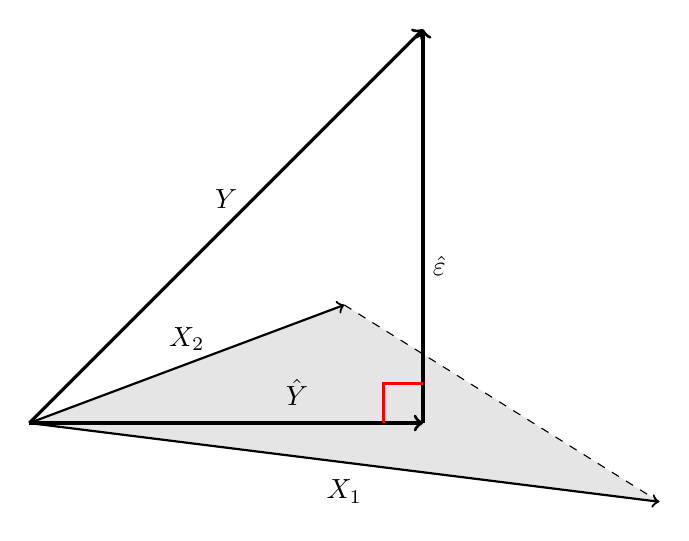
\begin{tikzpicture}[scale=0.5]
		\fill[black!10!white] (0,0)--(8,3)--(16,-2)--(0,0);
		\draw[->,thick] (0,0)--(8,3);
		\draw[->,thick] (0,0)--(16,-2);
		\draw[dashed] (8,3)--(16,-2);
		\draw[->,very thick] (0,0)--(10,10);
		\draw[->,very thick] (0,0)--(10,0);
		\draw[->,very thick] (10,0)--(10,10);
		\draw[red,very thick] (9,0)--(9,1)--(10,1);
		\node[above] at (5,5.2) {$Y$};
		\node[above] at (6.8,0.2) {$\hat{Y}$};
		\node[above] at (4,1.6) {$X_2$};
		\node[below] at (8,-1.2) {$X_1$};
		\node[right] at (10,4.) {$\hat{\varepsilon}$};
	\end{tikzpicture}
	\caption{Illustration of OLS as Projection}
	\label{fig:OLS_proj}
\end{figure}


\begin{corollary}
	\red{Sum of Squares Decomposition} It immediately follows from Pythagoras that 
	\[
	Y'Y = \hat{Y}'\hat{Y} + \hat{\varepsilon}'\hat{\varepsilon}
	\]
	Equivalently, SST $=$ SSE $+$ SSR or
	\[
	\sum_{i=1}^n Y_i^2 = \sum_{i=1}^n \hat{Y}_i^2 + \sum_{i=1}^n \hat{\varepsilon}_i^2
	\]
	It follows immediately that $R^2 = \text{SSE } / \text{ SST} \in [0,1]$. The extreme values of $R^2$ correspond to $\hat{Y} = 0$ and $\hat{\varepsilon} = 0$ respectively. It also follows that $\hat{\varepsilon}$ is \emph{by construction} orthogonal to $\hat{Y}$. 
\end{corollary}

We will recap this and basic related facts in the first homework.

\begin{question}
	What happens with collinear $X$?
\end{question}

With collinear $X$, the set on which we project is of lower dimension. The projection $\hat{Y}$ is still unique, but the projection coefficient is not.

\begin{definition}
	The \blue{projection coefficient} $\hat{\beta}$ is defined as 
	\[
	\hat{\beta} \equiv \argmin_b \sum_i (Y_i - X_i'b)^2 = \argmin_b (Y - Xb)' (Y - Xb) 
	\]
	and can be characterized by the first order condition
	\begin{align*}
		\frac{\partial }{\partial b} (Y - Xb)' (Y - Xb) &= -2X'Y + 2X'Xb \excleqq 0 \\
		\Longrightarrow \hat{\beta} &= (X'X)^{-1}X'Y
	\end{align*}
	The fitted values and residuals equal
	\begin{align*}
		\hat{Y} &= X\hat{\beta} = \underbrace{X(X'X)^{-1}X'}_{P_X\text{, the projection matrix}} Y = P_X Y \\
		\hat{\varepsilon} &= Y - \hat{Y} = (\underbrace{I_n - X(X'X)^{-1}X'}_{\text{annihilator matrix}})Y
	\end{align*}
\end{definition}

\begin{example}
	\red{\emph{Frisch-Waugh(-Lovell)}} The projection of $Y$ on $X$ can be decomposed, giving rise to some important results. To fix ideas, consider projecting $Y$:
	\begin{itemize}
		\item on the scalar $X_1$ (plus a constant), getting slope coefficient $\tilde{\beta}_1$, versus
		\item on the scalars $(X_1,X_2)$ (plus a constant), getting slope coefficients $(\hat{\beta}_1,\hat{\beta}_2)$.
	\end{itemize}
	Can we interestingly relate $\tilde{\beta}_1$ to $\hat{\beta}_1$? Yes! To do so, consider projecting $X_1$ on $X_2$, getting slope coefficient $\hat{\gamma}$. To simplify, assume all variables are demeaned. Across regressions, this leads to the first order conditions:
	\begin{align*}
		0 &= \expect_n \parl X_1 \parl Y - \hat{\beta}_1X_1 - \hat{\beta}_2X_2\parr\parr \\
		0 &= \expect_n \parl X_2 \parl Y - \hat{\beta}_1X_1 - \hat{\beta}_2X_2\parr\parr \\
		0 &= \expect_n \parl X_2 \parl X_1 - \hat{\gamma}X_2\parr\parr \\
	\end{align*}
	We can combine the first two, and use the third to get
	\begin{align*}
		0 &= \expect_n (X_1 - \hat{\gamma}X_2)\parl Y - \hat{\beta}_1X_1 - \hat{\beta}_2X_2\parr \\
		&= \expect_n (X_1 - \hat{\gamma}X_2)\parl Y - \hat{\beta}_1X_1 - \hat{\beta}_1 \hat{\gamma}X_2\parr \\
		&= \expect_n (X_1 - \hat{\gamma}X_2)\parl Y - \hat{\beta}_1 (X_1 - \hat{\gamma}X_2)\parr
	\end{align*}
	The last line is the first order condition from regressing $Y$ on the residuals of the regression of $X_1$ on $X_2$. Thus, $\hat{\beta}_1$ is the slope coefficient from that regression. We can extend this argument to show that $Y$ can be residualized as well.
	
	\begin{remark}
		If we think about this as if $X_1$ is schooling and $X_2$ is family income, we are essentially including only the uncorrelated parts of those variables through this method, and don't need to worry about the correlation between the two.
	\end{remark}
	
	When thinking about \blue{Omitted Variable Bias}, we can similarly characterize the projection of $X_2$ on $X_1$ by \[ 0 = \expect_n (X_1(X_2 - \tilde{\gamma}X_1)) = \expect_n \parl X_1\parl \hat{\beta}_2X_2 - \hat{\beta}_2 \tilde{\gamma}X_1\parr\parr\] We can then substitute the first order condition from above, and get \[0 = \expect_n \parl X_1 \parl Y - \hat{\beta}_1 X_1 - \hat{\beta}_2 X_2\parr \parr = \expect_n \parl X_1 \parl Y - \hat{\beta}_1 X_1 - \hat{\beta}_2\tilde{\gamma} X_1\parr \parr\] So we have the first order condition from regression $Y$ on $X_1$ only. We can conclude that the slope coefficient from that regression is \[\tilde{\beta} = \hat{\beta_1} + \tilde{\gamma} \hat{\beta}_2\] If there is a \blue{causal interpretation} of the projection of $Y$ onto $(X_1,X_2)$, then the difference term $\tilde{\gamma} \hat{\beta}_2$ is (the sample analog of) the \blue{omitted variable bias} incurred by omitting $X_2$. 
	
	\begin{remark}
		We haven't even really introduced the idea of random variables and expectation yet. The word \emph{bias} here is really loose, and doesn't make sense in the world of projection. However, in the real economic word, it makes a lot of sense in most contexts -- in that case, you are saying that the omitted variables systematically bias the estimator in some direction.
	\end{remark}
\end{example}

\begin{example}
	\red{\emph{Frisch-Waugh(-Lovell) General Statement}} We can now do the same thing, more generally. Partition as follows:
	\begin{align*}
		X = \matrixp{X_1 \\ X_2} \quad;\quad \expect XX' &\equiv Q = \matrixp{Q_{11} & Q_{12} \\Q_{21} & Q_{22}} = \matrixp{\expect X_1 X_1' & \expect X_1 X_2' \\ \expect X_2 X_1' & \expect X_2 X_2'} \\
		\expect XY &\equiv Q_{XY} = \matrixp{Q_{1Y} \\ Q_{2Y}} = \matrixp{\expect X_1Y \\ \expect X_2Y}
	\end{align*}
	and use notation $\hat{Q}_{11}$ (etc) for sample analogs. Then, it can be shown that
	\[
	\hat{\beta} = \matrixp{\parl \hat{Q}_{11} - \hat{Q}_{12}\hat{Q}_{22}^{-1}\hat{Q}_{21}\parr^{-1} \parl \hat{Q}_{1Y} - \hat{Q}_{12}\hat{Q}_{22}^{-1}\hat{Q}_{2Y}\parr \\ \parl \hat{Q}_{22} - \hat{Q}_{21}\hat{Q}_{11}^{-1}\hat{Q}_{12}\parr^{-1} \parl \hat{Q}_{2Y} - \hat{Q}_{21}\hat{Q}_{11}^{-1}\hat{Q}_{1Y}\parr}
	\]
	Regressing $X_1$ on $X_2$ would yield coefficients $\hat{\gamma} \equiv \hat{Q}_{22}^{-1}\hat{Q}_{21}$ and residuals $\hat{\eta} \equiv X_1 - X_2 \hat{Q}_{22}^{-1}\hat{Q}_{21}$. Hence, we have that \begin{align*} \expect_n \hat{\eta}^2 &= \expect_n X_1^2 + \hat{Q}_{12}\hat{Q}_{22}^{-1}\expect_n X_2^2  \hat{Q}_{22}^{-1}\hat{Q}_{21} - 2\expect_n X_1X_2  \hat{Q}_{22}^{-1}\hat{Q}_{21} \\ &= \hat{Q}_{11} - \hat{Q}_{12} \hat{Q}_{22}^{-1}\hat{Q}_{21}\end{align*} By similar algebra, $\expect_n \hat{\eta}Y = \hat{Q}_{1Y} -  \hat{Q}_{12}\hat{Q}_{22}^{-1}\hat{Q}_{2Y}$. It follows that if we projected $Y$ on the residual from regressing $X_1$ on $X_2$, we would get coefficient $\tilde{\beta}$, where
	\[
	\tilde{\beta}_1 = \parl \hat{Q}_{11} - \hat{Q}_{12} \hat{Q}_{22}^{-1}\hat{Q}_{21}\parr^{-1}\parl \hat{Q}_{1Y} - \hat{Q}_{12} \hat{Q}_{22}^{-1}\hat{Q}_{2Y}\parr = \hat{\beta}_1
	\] 
	
	\begin{remark}
		Verbally, the multivariate OLS coefficient on $X_1$ is the coefficient one would get by regressing $Y$ on the residual from regressing $X_1$ on all other covariates. We can show that this statement remains true if we replace $Y$ with the residual $Y - \mathcal{P}_{X_2}(Y)$, where $\mathcal{P}_{X_2}$ is the population projection onto $X_2$. This may look like a curiosity now, but is an important starting point for partially linear models and other such things. An immediate payoff is that if you recall it, you'll never forget the own-variance formula for multivariate regression coefficients.
	\end{remark}
\end{example}

There are two ways to interpret OLS. Neither of them are uniquely `right', but you should always be clear about which one you are appealing to. The \blue{Best Linear Prediction} is an interpretation that makes sense under extremely general conditions. It's the notion of a linear model that is generalized in most predictive (notably, data science / statistical learning) applications. The \blue{Causal (or Structural) Linear Model} is more demanding, but allows for causal interpretation. It's the notion of linear model that is generalized in most causal (for example, Instrumental Variables) applications. Note that this does not preclude predictive application of linear models as a component of causal inference. A salient example is the ``first stage'' in IV regression.

\paragraph{Best Linear Prediction.} Write $Y = m(X) + \varepsilon$, where $m(x) \equiv \expect(Y \mid X = x)$. That $\expect(\varepsilon \mid X) = 0$ is now a tautology. We can show that $b\opt \equiv (\expect XX')^{-1} \expect(XY)$, if it exists, minimizes $\expect(Y - X'b)^2$. That is, $\hat{Y} \equiv \mathcal{P}_XY \equiv X'b\opt$ is the \blue{best linear predictor under square loss}. Furthermore, under these conditions, $\expect Xe=0$, where $e \equiv Y - \mathcal{P}_X(Y)$, meaning that the projection error $e$ is not correlated with $X$.

\begin{theorem}
	If a weak law of large numbers applies to both $\frac{1}{n}\sum_{i=1}^n X_i X_i'$ and $\frac{1}{n}\sum_{i=1}^n X_iY_i$ and $\expect XX'$ is nonsingular, then $b\opt$ is uniquely defined and $\hat{\beta} \toprob b\opt$.
\end{theorem}
\begin{remark}
	The best linear predictor $\hat{Y}$ is uniquely defined even if $\expect XX'$ is singular. In that case, $b\opt$ is not unique. This is really important for models with lots of covariates -- think in statistical learning / machine learning.
\end{remark}

\paragraph{The (Causal/Structural) Linear Model} Write $Y = X'\beta + \varepsilon$, where $\expect(\varepsilon \mid X ) = 0$. Equivalently, $m(x) = \expect(Y \mid X = x) = x'\beta$. In this version, $\expect(\varepsilon \mid X) = 0$ is \emph{not} tautological! Our assumptions become much stronger. To be precise, we are assuming that (i) $\varepsilon$ is mean-independent of $X$, and (ii) the mean of $\varepsilon$ is zero. These are new assumptions! We pay a large cost, but there are also large benefits. This model allows for \blue{causal interpretation} of the estimand: in expectation, a change $\Delta X$ causes a corresponding change $\Delta X'\beta$ in $Y$. Importantly, this difference isn't just about interpretation -- some important results are only available under the stronger assumptions.

\begin{remark}
	Remember that within limits, a linear model can capture nonlinearities. Some examples: \begin{enumerate}
		\item Polynomial expansion: \[Y = \beta_0 + \beta_1 H + \beta_2 H^2 + \cdots + \varepsilon \]
		\item Log or log-log regression: \[\ln Y = \ln A + \alpha \ln K + (1-\alpha) \ln L + \cdots + \varepsilon\] (Note! This changes the necessary assumption on $\varepsilon$, as in the primal it is now multiplied by the covariates)
		\item Treatment effects with interactions: \[Y = \beta + \delta \cdot \text{treatment} + \gamma \cdot \text{female} \cdot \text{treatment} + \cdots + \varepsilon\]
	\end{enumerate}
	Indeed, many ``big data'' models are high-dimensional but linear! Think of basically any machine learning context.
\end{remark}

\paragraph{OLS as a Random Variable.}

The central questions are: What can we say about the estimator as a random variable? Are there conditions under which it has desirable properties, notably if our objective is to learn about $\beta$ (or possibly the population $\mathcal{P}_X(Y)$)?

Consider drawing $n$ samples and taking $\beta_i$, for $i \in \{1,\dots,n\}$ to be a random variable. If we show the histogram (in the slides) of these $\{\beta_i\}$, we can see that as $n$ increases they tend to look normal! However, this is not necessarily a central limit theorem. Actually, the distribution of the estimators will approach the distribution of the error terms as $n$ increases, under weaker assumptions. However, we assume normally distributed errors a lot.

\begin{remark}
	We had a small aside to wonder whether we think of the vertical squared distance between each point and the line, or the shortest distance between the point and the line squared. The second is actually different from OLS -- it's precisely \blue{principal component analysis}!
\end{remark}

\begin{remark}
	What if we minimized the horizontal distance? Then we would get the projection of $X$ onto $Y$ rather than \emph{vice versa} -- called \blue{reverse regression}. This is expanded on a lot in the first homework -- basically, the coefficients are normalized to the variances of $X$ and $Y$ respectively. They are the same if and only if $\var(X) = \var(Y)$. 
\end{remark}

\begin{remark}
	What if we minimize absolute values instead of squares? That would be \blue{median regression} -- at a population level, the median will solve this problem. By using other loss functions, we could tease out the other quantiles, and by using all of them we would get \blue{quantile regression}, where we treat the quantiles as being heterogeneously treated.
\end{remark}

For finite sample theory, we will make the following assumptions:

\begin{assumption}\label{ass:ols_finite}
	In data matrix notation, we have that \begin{enumerate}
		\item $Y = X\beta + \varepsilon$ \blue{`linearity'}
		\item $\expect(\varepsilon \mid X) = 0$ \blue{`strong exogeneity'}
		\item $\rank(X) = K$ a.s., where $X \in \reals^{n \times K}$ \blue{`rank condition'} (equivalent: $X'X$ nonsingular a.s.)
		\item $\expect(\varepsilon\varepsilon' \mid X) = \sigma^2 I_n$ \blue{`spherical error'}
	\end{enumerate}
\end{assumption}
The first two assumptions together imply a causal linear model. Assumptions that are natural when considering OLS as the `best linear predictor' do not suffice to attain unbiasedness of $\hat{\beta}$. These further imply that $\varepsilon$ is zero in expectation conditional on \emph{all} covariates -- including past and future realizations. That's quite strong, but matters a lot more in time series econometrics. If we assume the data are i.i.d., this is not stronger than the earlier assumption that they are independent vector-wise.

The third assumption is an identification condition, and will fail if any covariates are linearly dependent on each other. We already talked about this previously, but note that in finite samples we are immediately excluding discrete covariates! Though the probability may be small, it doesn't meet the criterion for almost surely. We may describe $\hat{\beta}$ as `conditionally unbiased', where we are conditioning on $X$.

Assumption four combines conditional uncorrelatedness and homoskedasticity of errors. The latter makes sense only in the causal model because, even if the true regression error $\varepsilon = Y - m(X)$ is homoskedastic, the projection error \[e = Y - \mathcal{P}_X(Y) = Y - m(X)+ m(X)-\mathcal{P}_X(Y) = \varepsilon + m(X) - \mathcal{P}_X(Y)\]is not.

We have a hidden assumption that $\expect \|X\|^2 < \infty$. This is an existence result, and not so strong generally -- if we assume $X$ is non-stochastic, nothing here relies on it. It is an assumption, however.

These assumptions give us the following theorems:

\begin{theorem}
	\red{Finite Sample Bias and Variance} Under Assumptions~\ref{ass:ols_finite}, we have that
	\begin{enumerate}
		\item $\expect\parl\hat{\beta} \mid X\parr = \beta$
		\item $\var\parl \hat{\beta} \mid X\parr = \sigma^2 (X'X)^{-1}$
	\end{enumerate}
	\ie $\hat{\beta}$ is unbiased and its variance is determined.
\end{theorem}
\begin{proof}
	We first observe that \[ \hat{\beta} = (X'X)^{-1}X'Y = (X'X)^{-1}X'(X\beta + \varepsilon) = \beta + \underbrace{(X'X)^{-1}X'\varepsilon}_{=\text{ estimation error}} \]Therefore, the first two claims are that 
	\begin{align*}
		\expect\parl \parl X'X\parr^{-1}X'\varepsilon \mid X\parr &= 0 \\ \var\parl \parl X'X\parr^{-1}X'\varepsilon \mid X\parr &= \sigma^2 (X'X)^{-1}
	\end{align*}
	We have directly that
	\[
	\expect\parl \parl X'X\parr^{-1}X'\varepsilon \mid X\parr = \parl X'X\parr^{-1}X'\underbrace{\expect(\varepsilon \mid X)}_{=0} = 0
	\]
	\[
	\var\parl \parl X'X\parr^{-1}X'\varepsilon \mid X\parr = (X'X)^{-1} X' \sigma^2I_n X' (X'X)^{-1} = \sigma^2 (X'X)^{-1}
	\]
\end{proof}

\begin{theorem}
	\red{Gauss-Markov Theorem} Under Assumptions	~\ref{ass:ols_finite}, if an estimator $\tilde{\beta}$ is linear (in $Y$) and unbiased, then \[\var(\tilde{\beta} \mid X) \ge \sigma^2 (X'X)^{-1}\]
\end{theorem}
\begin{proof}
	We assume that $\tilde{\beta} = CY$ for some $C$ (that may depend on $X$). Define $D \equiv C - (X'X)^{-1}X'$, and we have that
	\begin{align*}
		\beta &= \expect\parl ((X'X)^{-1}X' + D)Y \mid X\parr &&(\text{Unbiased}) \\ 
		&= \beta + \expect\parl DY \mid X\parr \\
		&= \beta + \expect \parl D(X\beta + \varepsilon) \mid X\parr \\
		&= \beta + \expect\parl DX\beta \mid X\parr + D\underbrace{\expect(\varepsilon \mid X)}_{=0} \\&\Longrightarrow\expect(DX\beta \mid X) = 0
	\end{align*}
	This result is only possible if conditional on $X$ the expression $DX\beta$ is non-stochastic -- we have that $DX\beta = 0$ for any $\beta$! This holds only if $DX = 0$. So finally, we have
	\begin{align*}
		\var(\tilde{\beta} \mid X) &= \var\parl ((X'X)^{-1}X' + D)Y \mid X\parr \\
		&= \var\parl ((X'X)^{-1}X' + D)(X\beta_0 + \varepsilon) \mid X\parr \\
		&= \var\parl ((X'X)^{-1}X' + D) \varepsilon \mid X\parr \\
		&= \sigma^2 ((X'X)^{-1}X' + D)((X'X)^{-1}X' + D)' \\
		&= \sigma^2 \parl (X'X)^{-1}X'X (X'X)^{-1} + DX(X'X)^{-1} + (X'X)^{-1}X'D' + DD'\parr \\
		&\ge \sigma^2 (X'X)^{-1} = \var(\hat{\beta})
	\end{align*}
	where the conclusion follows from the fact that $DD'$ is positive semi-definite.
\end{proof}


\begin{question}
	Is homoskedasticity necessary for this result? 
\end{question}
\begin{answer}
	Yes! Consider the case where $\expect \varepsilon\varepsilon' = \Omega$ is known and diagonal but its diagonal entries are not the same. Then the Gauss-Markov assumptions apply to the transformed model \[\Omega^{-\frac{1}{2}}Y = \Omega^{-\frac{1}{2}}X +  \Omega^{-\frac{1}{2}}\varepsilon\] so the estimator \[\hat{\beta}_{WLS} = (X'\Omega^{-1}X)^{-1}X' \Omega^{-1}Y\]is the best linear unbiased estimator. However, $\hat{\beta}_{WLS} = \hat{\beta}$ if and only if $\Omega = \sigma^2 I_n$ for some $\sigma^2$. This is called the \blue{Weighted Least Squares} estimator, which in this case would perform better than OLS.
\end{answer}

\paragraph{Some important closed-form expressions} Consider a simple linear regression $Y = \alpha + \beta X + \varepsilon$. Then we have that: \[ \hat{\beta} = \frac{\sum_{i=1}^n (X_i - \bar{X})(Y_i - \bar{Y})}{\sum_{i=1}^n (X_i - \bar{X})^2} = \frac{\sum_{i=1}^n (X_i - \bar{X})Y_i}{\sum_{i=1}^n (X_i - \bar{X})X_i}\]\[\var\parl\hat{\beta} \mid X\parr = \frac{\sigma^2}{\sum_{i=1}^n (X_i-\bar{X})^2}\]where $\sigma^2$ is the variance of $\varepsilon$. In a multivariate regression, the variance of the $k$th component of $\hat{\beta}$ is \[\var\parl \hat{\beta}_k \mid X\parr = \frac{\sigma^2}{(1-R_k^2) \sum_{i=1}^n (X_{ki} - \bar{X}_k)^2}\] where $R_k^2$ is the $R^2$ of the regression of $X_k$ on the other covariates. Why is this obvious? Frisch-Waugh-Lovell, of course! The factor $1 / (1-R_k^2)$ is sometimes called the \blue{variance inflation factor (VIF)}. 
	
	\begin{remark}
		Know the expression for the variance of the $k$th component of $\hat{\beta}$ by heart! You should internalize it from Frisch-Waugh-Lovell.
	\end{remark}
	
	We also have sample analogs and estimators for $\sigma^2$: The \blue{sample analog} (which is a \blue{method of moments estimator}) of $\sigma^2$ is \[\hat{\sigma}^2 \equiv \frac{1}{n} \hat{\varepsilon}' \hat{\varepsilon} = \frac{1}{n} \sum_{i=1}^n \hat{\varepsilon}_i^2\]However, we can also show (exercise?) that $\expect(\hat{\sigma}^2 \mid X ) = \frac{n-K}{n}\sigma^2$. Why? Heuristically, the random variable $\hat{\varepsilon}$ has only $(n-K)$ degrees of freedom because it is constrained by the $K$ equations $X'\hat{\varepsilon} = 0$. It is more common to use the unbiased \[s^2 \equiv \frac{1}{n-K}\sum_{i=1}^n \hat{\varepsilon}_i^2\]
	
	Estimators of the standard deviation are often important. We will call them \blue{standard errors}. $\sqrt{s^2}$ is the standard error of the regression, and $SE(\hat{\beta}) = (s^2 \matrixc{(X'X)^{-1}}_{kk})^{1/2}$ is the standard error of $\hat{\beta}_k$.
	
	\begin{remark}
		We \textbf{cannot} claim that these estimators are unbiased! Further, the use of `standard error' is dominant in econometrics, but other disciplines\footnote{Statistics...} `standard error' and `[sampling] standard deviation' may be synonyms. In this case, we use `\emph{estimated} standard errors'.
	\end{remark}
	
	\begin{remark}
		The spherical error assumption was only (fully) used for the variance expressions (and Gauss-Markov). Recall that from the algebra: \begin{align*} \hat{\beta} &= \beta + \underbrace{(X'X)^{-1}X'\varepsilon}_{=\text{estimation error}} \\ \Longrightarrow \var(\hat{\beta} \mid X) &= (X'X)^{-1}X' \underbrace{\expect (\varepsilon \varepsilon' \mid X)}_{=D}X(X'X)^{-1}\end{align*}Spherical error ($D = \sigma^2 I_n$) leads to simplification, but as long as we can estimate $D$, it is not necessary. Recall that \[\var(\hat{\beta} \mid X) = (X'X)^{-1}\parl \sum_{i=1}^n X_iX_i'\varepsilon_i^2\parr (X'X)^{-1}\]Assuming only heteroskedasticity (\ie $D$ remains diagonal), we have the \blue{oracle estimator} \[\hat{\var}_{\text{oracle}}(\hat{\beta} \mid X) \equiv (X'X)^{-1} \parl \sum_{i=1}^n X_iX_i'\varepsilon_i^2\parr (X'X)^{-1}\]This is an unbiased estimator, but is not available. Plugging in $\hat{\varepsilon}_i$ leads to a plausible estimator:\[\hat{\var}_{\text{HC0}}(\hat{\beta} \mid X) \equiv (X'X)^{-1} \parl \sum_{i=1}^n X_iX_i'\hat{\varepsilon}_i^2\parr (X'X)^{-1}\]This is biased, which motivates a degree of freedom adjustment:\[\hat{\var}_{\text{HC1}}(\hat{\beta} \mid X) \equiv \frac{n}{n-K}(X'X)^{-1} \parl \sum_{i=1}^n X_iX_i'\hat{\varepsilon}_i^2\parr (X'X)^{-1}\]There are a ton of similar estimators. HC0 is the original (Eicker-White) heteroskedasticity robust variance estimator, and HC1 is the industry standard (\ie it is the STATA default). Neither is obviously best, and Hansen has some other options. In applied work, these are dominant because homoskedasticity is rarely plausible. Using weighted least squares is technically possible, but rarely used because it requires knowing \emph{ex ante} the structure of the heteroskedasticity. Clustered standard errors are similar to this, though we omit them for now.
	\end{remark}
	
	From here on, we will make the following (strong) assumption:
	\begin{assumption}\label{ass:errors_normal}
		$\varepsilon$ has a normal distribution: \[(\varepsilon\mid X) \sim \normal(0,\sigma^2I_n)\]
	\end{assumption}
	
	With this, we have the following:
	
	\begin{theorem}
		Define $s^2 = \frac{(Y-X\beta)'(Y-X\beta)}{n-K}$ and let the matrix $R \in \reals^{r \times K}$ have maximal rank $r \le K$. Under Assumptions~\ref{ass:ols_finite} and \ref{ass:errors_normal}, we then have \[(\hat{\beta}-\beta) \mid X \sim \normal(0,\sigma^2(X'X)^{-1})\]and:\begin{align*} t\textnormal{--ratio} = t &\equiv \frac{\hat{\beta}_k - \beta_k}{	\parl s^2 \matrixc{(X'X)^{-1}}_{kk}\parr^{1/2}} \sim t_{n-K} \\ F\textnormal{--statistic} = F &\equiv \frac{(R\hat{\beta} - R\beta)' (R(X'X)^{-1}R')^{-1}(R\hat{\beta} - R\beta)}{s^2r} \sim F_{r,n-K} \end{align*}Thus, the null hypothesis $\hyp_0: R\beta = r$ can be tested with exact size control by comparing \[\frac{(R\hat{\beta} - r)' (R(X'X)^{-1}R')^{-1}(R\hat{\beta} - r)}{s^2r}\]to the relevant quantiles of $F_{r,n-K}$, etc.
	\end{theorem}
	\begin{proof}
		The first part, from section: We showed earlier that $\hat{\beta} = \beta + (X'X)^{-1}X'\varepsilon$, so \[\expect[\hat{\beta} - \beta \mid X] = \expect[\hat{\beta} \mid X ] - \beta = \beta + (X'X)^{-1}X' \underbrace{\expect[\varepsilon \mid X] }_{=0} - \beta = 0\]
		and \[\var(\hat{\beta} - \beta \mid X) = \var(\hat{\beta} \mid X) = \sigma^2 (X'X)^{-1}\]Conclusion follows by also noting that the sum of normally-distributed random variables.
		
		The rest follows directly from the definitions of the relevant distributions, and our assumptions on $R$.
	\end{proof}
	
	\begin{remark}
		Recall that the $t$-distribution converges quickly to the standard normal as degrees of freedom increase, but the quantiles (and thus associated critical values) can be quite different under small degrees of freedom.
	\end{remark}

\newpage
\section{The Linear Model in Large Samples}

We will now look at large sample (asymptotic) theory; results will be weaker in that they maximally only hold \emph{almost surely} (\ie we care about stochastic convergence). However, our assumptions are also a lot weaker:

\begin{assumption}\label{ass:asymptotic_ols}
	$(X,Y)$ are i.i.d., $\expect Y^2 < \infty$ and $\expect \|X\|^2 < \infty$, and $\expect(XX')$ is positive definite.
\end{assumption}

\begin{remark}
	These assumptions suffice for the projection coefficient to be well-defined: $b\opt \equiv (\expect XX')^{-1} \expect XY$. We have:
\end{remark}

\begin{theorem}
	Under Assumptions~\ref{ass:asymptotic_ols}, we have: \[\hat{\beta} \equiv (\expect_n XX')^{-1}\expect XY \toprob b\opt\]
\end{theorem}
\begin{proof}
	By the weak law of large numbers, we have that $\expect_n XX' \toprob \expect XX'$ and $\expect_n XY \toprob \expect XY$. By the Continuous Mapping Theorem, it follows that $(\expect_n XX')^{-1} \toprob (\expect XX')^{-1}$, since as $n$ increases $\expect_n XX'$ is nonsingular with probability approaching 1. The claim follows directly from Slutsky's Theorem.
\end{proof}

We have not yet used any assumptions that set the structural linear model apart from the best linear predictor under square loss interpretation, but we've made no causal claims. However, the asymptotics apply to both! 

We must assume the following to make causal claims, if the linear model $Y = X'\beta + \varepsilon$ is maintained:
\begin{assumption}\label{ass:asymptotic_causal}
	$\expect X\varepsilon = 0$, also called \blue{predetermination}. Additionally, we strengthen the moment assumption: $\expect Y^4 < \infty$ and $\expect \|X\|^4 < \infty$.
\end{assumption}
\begin{remark}
	This is significantly weaker than the unbiasedness assumption -- we only need that $\varepsilon$ is uncorrelated with the contemporaneous regressors. This ensures that $b\opt = \beta$ (and, by implication, consistency): \[b\opt = (\expect XX')^{-1}\expect XY = (\expect XX')^{-1}\expect X(X'\beta + \varepsilon) = \beta + (\expect XX')^{-1}\expect X\varepsilon = \beta\]
	We could alternatively show consistency from scratch using this assumption, the way Hayashi does.
\end{remark}

To look at the asymptotic distribution, note that
\begin{align*}
	\hat{\beta} &= (\expect_n XX')^{-1} \expect_n XY = (\expect_n XX')^{-1} \expect_n X(Xb\opt + e) \\ \Longrightarrow \hat{\beta} - b\opt &= (\expect_n XX')^{-1}\expect_n Xe 
\end{align*}
where $b\opt$ is the population projection coefficient and $e$ is the (true underlying) projection error. By predetermination, $(\expect_n XX')^{-1}\expect_n Xe \toprob 0$. However, there is the suggestion of an asymptotic result -- it seems natural that \[\sqrt{n}(\expect_n Xe) \todist \normal(0,\Omega) = \normal(0,\expect(XX'e^2))\]where the last equality just defines $\Omega$. If that were the case, we would easily have that \[\sqrt{n}(\hat{\beta} - b\opt) \todist \normal(0,(\expect XX')^{-1}\Omega (\expect XX')^{-1})\]This derivation is basically true.\footnote{`Morally true' - J\"{o}rg} We just need to ensure that all terms exist. For this, our stronger Assumptions~\ref{ass:asymptotic_causal} suffice. If the kurtosis exists, we can argue that $\Omega$ is finite, by repeatedly using Cauchy-Schwartz. For any one element of $\Omega$,
\begin{align*}
	|\expect (X_kX_\ell e^2)| &\le \expect |X_kX_\ell e^2| = \expect ( |X_k||X_\ell| |e^2|) \\&\le (\expect X_k^2 X_\ell^2)^{1/2} (\expect e^4)^{1/2} \le (\expect X_k^4)^{1/4} (\expect X_\ell^4)^{1/4} (\expect e^4)^{1/2} < \infty
\end{align*}
we finish by writing \[\sqrt{n}(\hat{\beta} - b\opt) \todist (\expect XX')^{-1}\normal(0,\Omega) = \normal (0,(\expect XX')^{-1} \Omega (\expect XX')^{-1})\]
where we again use Slutsky and the properties of normal distributions. Formally, we have:

\begin{theorem}
	With Assumptions~\ref{ass:asymptotic_ols} and Assumptions~\ref{ass:asymptotic_causal}, we have that 
	\begin{align*}
		\sqrt{n}(\hat{\beta} - b\opt) &\todist \normal(0,\avar(\hat{\beta})) \\
		\text{where } \avar(\hat{\beta}) &= (\expect XX')^{-1} \Omega (\expect XX')^{-1}) \\ [&= Q_{XX}^{-1} \Omega Q_{XX}^{-1} = \Sigma_{XX}^{-1} \Omega \Sigma_{XX}^{-1}]
	\end{align*}
\end{theorem}
\begin{proof}
	A generalization of above.
\end{proof}
\begin{remark}
	Note that we are \emph{not} assuming a linear model here! We actually get this result under relatively limited assumptions, we only need that the moment conditions exist. If we want to get inference results, we need more, but as a projection result this still holds.
\end{remark}

\begin{definition}
	aVar is the \blue{asymptotic variance}, the variance of the limiting distribution. In general, this is not necessarily the asymptotic limit of an estimator's squared variance, though the current assumptions suffice.
\end{definition}

\begin{remark}
	This theorem provides the \emph{joint} asymptotic distribution of estimates. The information contained in joint normality is relevant for:
	\begin{enumerate}
		\item Inference on a linear combination of estimates, \eg their sum or difference. This could also be achieved by reparameterization, but that's impractical.
		\item Joint inference, \ie confidence ellipsoids, on several coefficients
		\item Inference on a known, differentiable function of $\beta$ through the Delta method (conceptually straightforward, but very important in practice! See the textbook for an example worked through)
		\item Conservative inference on a known, nondifferentiable function of $\beta$ through projection (\ie operate the function on ever $b$ in the confidence ellipsoid). In structured cases, you may be able to improve on this -- ask J\"{o}rg if this question arises in your research!
	\end{enumerate}
\end{remark}

\begin{remark}
	Results in this course hold pointwise as $n \to \infty$ for \emph{given} parameter values, not \emph{uniformly} over parameter values. How big of a problem is this? With some more effort, most results in this course are available uniformly in `nice' cases. However, there are several cases that are not nice and are empirically relevant: (i) estimators that can be corner solutions of their problems, (ii) estimation of maxima, (iii) rare events, and (iv) post-model selection estimation and inference. In these, pointwise perspectives can be quite misleading. 
\end{remark}

\begin{theorem}
	Under Assumptions~\ref{ass:asymptotic_ols} and Assumptions~\ref{ass:asymptotic_causal}, we have that \[\hat{\avar}_{HC0} \equiv (\expect_n XX')^{-1} \hat{\Omega} (\expect_n XX')^{-1} \toprob \avar(\hat{\beta})\]where $\hat{\Omega} \coloneqq \expect_n[XX'\hat{\varepsilon}^2]$, and similarly for $HC1$, and so on. Basically, all of these are consistent.
\end{theorem}
\begin{proof}
	(Sketch) The bottleneck is the consistency of $\hat{\Omega}$. Write: \[\hat{\Omega} = \frac{1}{n}\sum_{i=1}^n X_i X_i \hat{e}_i^2 = \underbrace{\frac{1}{n}\sum_{i=1}^n X_i X_i' e_i^2}_{\toprob \Omega} + \underbrace{\frac{1}{n}\sum_{i=1}^n X_i X_i (\hat{e}_i^2 - e_i^2)}_{\toprob 0}\]That the rightmost term disappears can be shown through (tedious) repeated use of Cauchy-Schwartz and H\"{o}lder.
\end{proof}

\begin{proof}
	(Assuming Homoskedasticity) If we assume that $\expect(e^2 \mid X) = \sigma^2$, then we have the simplification \[\avar(\hat{\beta}) = (\expect XX')^{-1}\sigma^2\]and showing the consistency of \[\hat{\avar}(\hat{\beta}) = (\expect XX')^{-1} s^2\]is simple, and requires weaker assumptions (specifically, second moments suffices). However, recall that this makes sense only for a structural linear model (and is still restrictive).
\end{proof}


\paragraph{Inference.} Let $r: \reals^k \to \reals$ be a continuously differentiable function with $\nabla r(\cdot) = R(\cdot)$ (the easiest example is where $r$ extracts a component of $\beta$). Define $\theta = r(\beta)$ and $\hat{\theta} = r(\hat{\beta})$. By Delta Method, standard convergence results, and Slutsky, we have 
\begin{align*} 
	\sqrt{n}(\hat{\theta} - \theta) &\todist \normal(0,\avar(\hat{\theta})) \\
	\avar(\hat{\theta}) &= R(\beta) \avar(\hat{\beta})R(\beta)' \\
	\hat{\avar}(\hat{\theta}) \equiv  R(\hat{\beta}) \avar(\hat{\beta})R(\hat{\beta})' &\toprob R(\beta) \avar(\hat{\beta})R(\beta) \\ 
	\Longrightarrow t(\theta) \equiv \frac{\hat{\theta}-\theta}{SE(\hat{\theta})} \equiv \frac{\sqrt{n}(\hat{\theta}-\theta)}{\parl R(\hat{\beta})\hat{\avar}(\hat{\beta}) R(\hat{\beta})'\parr^{1/2}} &\todist \normal(0,1)
\end{align*}
This is the asymptotic $t$-statistic. For this to hold, we need that $\avar(\hat{\theta})$ is finite. A sufficient condition is that $R(\beta) \ne 0$ and that $\avar(\hat{\beta})$ has full rank.

\begin{definition}
	Dividing by the standard error like this is called \blue{studentization}. It ensures that the asymptotic distribution does not depend on unknown parameters, ensuring that the $t$-statistic (and others) are \blue{asymptotic pivots}.
\end{definition}

The previous result lets us create hypothesis tests and confidence intervals where the asymptotic sizes converge. Let $\Phi(\cdot)$ denote the standard normal cdf and define the quantiles $\Phi^{-1}(1-\alpha) \coloneqq c_\alpha$. Then
\begin{align*}
	\prob\{|t(\theta)| \le c_{\alpha / 2}\}&\toprob 1-\alpha \\
	\prob\{t(\theta) \in CI_\alpha(\theta)\} &\toprob 1-\alpha \\
	CI_\alpha(\theta) &= \barl \hat{\theta} - c_{\alpha / 2}\cdot SE(\hat{\theta}), \hat{\theta} + c_{\alpha / 2}\cdot SE(\hat{\theta})\barr
\end{align*}
and we compute one-sided confidence intervals similarly. If $r(\beta) = p'\beta$ for some known vector $p$, then $R(\cdot) = p'$ and the $t$-statistic simplifies to \[t(\theta) \equiv \frac{\hat{\theta}-\theta}{SE(\hat{\theta})} = \frac{\sqrt{n}(\hat{\theta}-\theta)}{\parl p' \hat{\avar}(\hat{\beta}) p\parr^{1/2}}\]If $p$ is a basis vector, this further simplifies the $t$-statistic for an individual coefficient. Choices like $p = (0,1,-1,0,\dots,0)$ lets us test the equality of two coefficients.

Under the causal linear model, another application is to $p = x$, in which case $\theta = \expect(Y \mid X = x)$, which is called a \blue{regression interval}. Note that the standard error depends on $x$ and will be smaller for more central values of $x$. 

\begin{remark}
	The regression interval is \emph{not} a forecast confidence interval! For forecast intervals, we must take $\varepsilon_t$ into account.
\end{remark}


We can generalize this to $\theta = r(\beta)$ where $r: \reals^k \to \reals^q$ is vector-valued. With this, $R(\cdot)$ is now the Jacobian of $r$, we have that 
\begin{align*}
	\sqrt{n}(\hat{\theta} - \theta) &\todist \normal(0,\avar(\hat{\theta})) \\
	\avar(\hat{\theta}) &= R(\beta) \avar(\hat{\beta})R(\beta)' \\
	\hat{\avar}(\hat{\theta}) \equiv  R(\hat{\beta}) \avar(\hat{\beta})R(\hat{\beta})' &\toprob R(\beta) \avar(\hat{\beta})R(\beta) \\ 
	\Longrightarrow W(\theta) \equiv \sqrt{n}(\hat{\theta}-\theta)' (\hat{\avar}(\hat{\theta}))^{-1} \sqrt{n}(\hat{\theta}-\theta) &\todist \chi_q^2
\end{align*}
This is the \blue{Wald} statistic. It can induce confidence regions similarly to the confidence intervals above -- however these are ellipsoids. These will be appropriate if one is genuinely interested in simultaneous inference of several scalars, and their projections onto the axes will be valid but (possibly very) conservative confidence intervals.

\begin{remark}A sufficient condition for this to hold is that both $R(\beta)$ and $\avar(\hat{\beta})$ are full-rank, which would mean that the hypotheses must be (locally) linearly independent at the truth -- for linear hypotheses, this is easy to check and a global property. \end{remark}

\newpage
\section{Instrumental Variables}

\begin{remark}
	Instrumental variables are of huge importance across economics, and are one of the greatest contributions of econometrics to empirical methods across science. They are actively used in causal inference across disciplines, specifically in biostatistics. Their appeal is that they allow for causally interpretable estimates if we think that (i) the linear model (or generalizations) is structural so $\beta$ has causal interpretation, but (ii) $\varepsilon$ correlates with $X$, because it absorbs relevant omitted variables. Of course, this remarkable result requires strong assumptions.
\end{remark}

\begin{model}
	For simplicity, consider simple linear regression \[Y = \beta_0 + \beta_1 X + \varepsilon\]where we cannot assets that $\expect X\varepsilon = 0$. The interpretation is that $\beta_1$ has a causal interpretation, but we could not estimate all relevant covariates. Now suppose that we have a random variable $Z$ with the following properties:\[\underbrace{\cov(Z,X) \ne 0}_{\text{Relevance}}\qquad \text{ and } \qquad \underbrace{\cov(Z,\varepsilon) = 0}_{\text{Validity}}\]This implies that \[\frac{\cov(Z,Y)}{\cov(Z,X)} = \frac{\beta_1 \cov(Z,X) + \cov(Z,\varepsilon)}{\cov(Z,X)} = \beta_1\]
\end{model}

\begin{example}
	(\href{https://www.aeaweb.org/articles?id=10.1257/000282803321455296}{Ginburgh \& van Ours (2003)}) $Y$ is the career success of a classical musician, $X$ is their placement in a prestigious competition for young musicians, and $Z$ is the order of appearance at the competition. The effect of $X$ on $Y$ is interesting, but `talent' impacts both. However, appearing late in the competition (verifiably) predicts success! Since order of appearance is random, it serves as an \blue{instrumental variable} (or just \blue{instrument}).
\end{example}

\begin{definition}
	\blue{Relevance} requires that $\cov(Z,X) \ne 0$. We need there to be some instrument-induced variation to play around with. Otherwise, we could pay a research assistant to flip coins all day and use that as an instrument. 
	
	Relevance must be \textbf{testable}. The covariance is consistently estimated with its sample analog. Indeed, it is standard practice to report the $F$-statistic from a `first-stage regression' of $X$ on $Z$.
\end{definition}

\begin{definition}
	\blue{Validity} requires that $\cov(Z,\varepsilon) = 0$. We need the instrument-induced variation to be exogenous. Otherwise, we could just use $X$ as an instrument for itself. 
	
	Validity is \textbf{not testable}. This will change once we have more instruments than regressors.
\end{definition}


\begin{definition}
	We can illustrate causal models using \blue{Directed Acyclic Graphs (DAG)}. Arrows read as `causes...'. The traditional OLS graph is Figure~\ref{fig:ols_dag}.
	
	\begin{figure}[H]
		\centering
		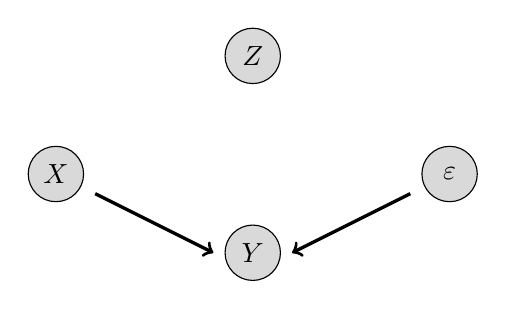
\begin{tikzpicture}[scale=0.5]
			\filldraw[black!15] (0,5) circle(20pt);
			\draw[black] (0,5) circle(20pt);
			\filldraw[black!15] (0,0) circle(20pt);
			\draw[black] (0,0) circle(20pt);
			\filldraw[black!15] (5,2) circle(20pt);
			\draw[black] (5,2) circle(20pt);
			\filldraw[black!15] (-5,2) circle(20pt);
			\draw[black] (-5,2) circle(20pt);
			
			\node at (0,5) {$Z$};
			\node at (0,0) {$Y$};
			\node at (5,2) {$\varepsilon$};
			\node at (-5,2) {$X$};
			
			%\draw[->, very thick] (4,2)--(-4,2);
			\draw[->, very thick] (-4,1.5)--(-1,0);
			\draw[->, very thick] (4,1.5)--(1,0);
		\end{tikzpicture}
		\caption{OLS DAG. The r.v. $Z$ plays no role, and $\cov(X,\varepsilon) = 0$.}
		\label{fig:ols_dag}
	\end{figure}

If $X$ is \blue{endogenous}, the DAG may look like Figure~\ref{fig:confound_dag}.

\begin{figure}[H]
		\centering
		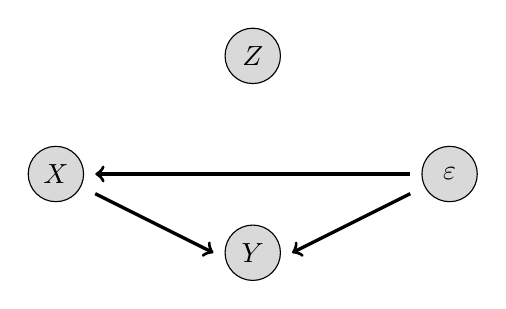
\begin{tikzpicture}[scale=0.5]
			\filldraw[black!15] (0,5) circle(20pt);
			\draw[black] (0,5) circle(20pt);
			\filldraw[black!15] (0,0) circle(20pt);
			\draw[black] (0,0) circle(20pt);
			\filldraw[black!15] (5,2) circle(20pt);
			\draw[black] (5,2) circle(20pt);
			\filldraw[black!15] (-5,2) circle(20pt);
			\draw[black] (-5,2) circle(20pt);
			
			\node at (0,5) {$Z$};
			\node at (0,0) {$Y$};
			\node at (5,2) {$\varepsilon$};
			\node at (-5,2) {$X$};
			
			\draw[->, very thick] (4,2)--(-4,2);
			\draw[->, very thick] (-4,1.5)--(-1,0);
			\draw[->, very thick] (4,1.5)--(1,0);
		\end{tikzpicture}
		\caption{OLS DAG. The r.v. $Z$ plays no role, but $\cov(X,\varepsilon) \ne 0$.}
		\label{fig:confound_dag}
	\end{figure}
	
The typical DAG representation of instrumental variables is Figure~\ref{fig:inst_dag}.

\begin{figure}[H]
		\centering
		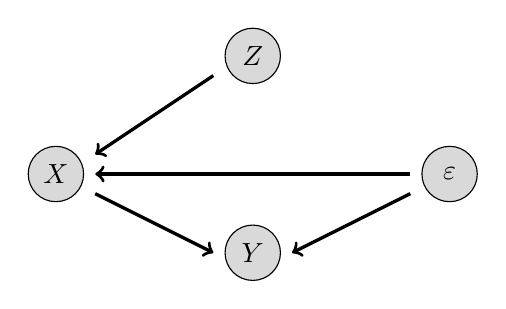
\begin{tikzpicture}[scale=0.5]
			\filldraw[black!15] (0,5) circle(20pt);
			\draw[black] (0,5) circle(20pt);
			\filldraw[black!15] (0,0) circle(20pt);
			\draw[black] (0,0) circle(20pt);
			\filldraw[black!15] (5,2) circle(20pt);
			\draw[black] (5,2) circle(20pt);
			\filldraw[black!15] (-5,2) circle(20pt);
			\draw[black] (-5,2) circle(20pt);
			
			\node at (0,5) {$Z$};
			\node at (0,0) {$Y$};
			\node at (5,2) {$\varepsilon$};
			\node at (-5,2) {$X$};
			
			\draw[->, very thick] (4,2)--(-4,2);
			\draw[->, very thick] (-4,1.5)--(-1,0);
			\draw[->, very thick] (4,1.5)--(1,0);
			\draw[->,very thick] (-1,4.5)--(-4,2.5);
		\end{tikzpicture}
		\caption{IV DAG. $\cov(Z,X) \ne 0$, $\cov(Z,\varepsilon) = 0$, and $\cov(X,\varepsilon) \ne 0$.}
		\label{fig:inst_dag}
	\end{figure}
\end{definition}

\begin{example}
	Instrumental variables in medical statistics: \red{Mendelian randomization} is an instrumental variables technique. The idea is that, in our terminology, genetic variation exogenous. Think about $Y = $ coronary disease, $X = $ HDL cholesterol level, and $\varepsilon = $ confounders (of which there are many -- diet and lifestyle heavily affect HDL cholesterol level). If we have some genetic variant $Z$ that increases HDL cholesterol level, we can use that as an instrument. The bottleneck assumption is that $Z$ affects \emph{only} HDL cholesterol level, not coronary disease.
\end{example}

\begin{example}
	Some famous\footnote{Note! Famous $\ne $ good!} examples:
	\begin{enumerate}
		\item \href{https://scholar.harvard.edu/files/stock/files/tariff_appendixb.pdf}{Wright (1928)} was the first example -- he wanted to estimate supply and demand elasticities for vegetable oils, but realized that quantities and prices are equilibrium quantities and prices, so endogenous. He used demand shifters (price changes of substitutes) and supply shifters (weather) as instruments. He averaged the estimators, which is something we would do now.
		\item \href{https://www.jstor.org/stable/2937954?seq=1}{Angrist \& Krueger (1991)} aim to estimate the returns to compulsory schooling, but selection into schooling is correlated. They instrument it by quarter of birth, where a different quarter may lead to another year `exposed' to compulsory schooling.
		\item \href{https://www.jstor.org/stable/116844}{Angrist \& Evans (1998)} want to estimate the effect of having children on female labor force participation, but the decision to have children is endogenous. They instrument with gender of children -- this is clearly random, but some parents prefer to have children of both genders so if they have two of the same, they are more likely to have a third than if the two are different genders.
		\item \href{https://davidcard.berkeley.edu/papers/geo_var_schooling.pdf}{Card (1993,5)} looks to estimate the returns to college education, but college attendance is endogenous. He instruments college attendance with distance from a college growing up, which may be pivotal in attendance decisions.
	\end{enumerate}
\end{example}


\begin{definition}
	We will derive the IV estimator as a \blue{Generalized Method of Moments (GMM)} estimator. Recall the method of moments: If we assume \[Y = X'\beta + \varepsilon ,\expect X\varepsilon = 0 \Longrightarrow \expect(X(Y - X'\beta)) = 0\]then a natural idea for estimating $\beta$ is to solve the empirical moment condition \[\expect_n (X(Y-X'\hat{\beta})) = 0\]which clearly yields the OLS estimator (as the above is the FOC of the minimization problem). However, if we assume that $\expect X\varepsilon \ne 0$, then OLS will be inconsistent for $\beta$ because it will estimate the projection coefficient \[b\opt = (\expect XX')^{-1}\expect XY = \beta + (\expect XX')^{-1} \expect X\varepsilon\]However, if we also observe a random $k$-vector $Z$ with $\expect Z\varepsilon = 0$ and $\rank(\expect ZX')=k$, then we have the moment condition \[\expect (Z(Y-X'\beta)) = 0 \Longrightarrow \beta = (\expect ZX')^{-1} \expect ZY\]where the assumptions assume that this is well-defined. Naturally, the estimator is \[\hat{\beta}_{IV} = (\expect_n ZX')^{-1} \expect_n ZY\]Note that \[\hat{\beta}_{IV} = (\expect_n ZX')^{-1} \expect_n ZY = (\expect_n ZX')^{-1} \expect_n Z(X'\beta + \varepsilon)= \beta + \underbrace{(\expect_nZX')^{-1} \expect_n Z\varepsilon}_{=\text{ estimation error}}\]From here, consistency follows essentially directly as $\expect_n Z\varepsilon \toprob 0$. However, we cannot claim unbiasedness, even if we assume the stronger that $\expect(\varepsilon \mid Z) = 0$. We will defer asymptotic theory until later. Note that some components of $Z$ may also appear in $X$, because if some elements of $X$ are unassociated with $\varepsilon$, they can act as their own instruments. By setting $Z = X$, we consider OLS as the special case of $X$ instrumenting itself.
\end{definition}

In the simple linear model, when $X$ and $Z$ are scalars, the IV slope estimator can be expressed as \[\frac{\sum_{i=1}^n (Z_i - \bar{Z})(Y_i - \bar{Y})}{\sum_{i=1}^n (Z_i - \bar{Z})(X_i - \bar{X})}\]The data matrix expression is, naturally, $\hat{\beta}_{IV} = (Z'X)^{-1}Z'Y$. For an application, consider regressing $X$ on $Z$ and then $Y$ on $\hat{X}$. In data matrix notation, we have 
\begin{align*}
	\tilde{\beta} &= (\hat{X}'\hat{X})^{-1}\hat{X}'Y \\ &= ((Z(Z'Z)^{-1}Z'X)'(Z(Z'Z)^{-1}Z'X))^{-1}(Z(Z'Z)^{-1}Z'X)'Y \\&= (X'Z(Z'Z)^{-1}Z'Z(Z'Z)^{-1}Z'X)^{-1}X'Z(Z'Z)^{-1}Z'Y \\ &= (X'Z(Z'Z)^{-1}Z'X)^{-1}X'Z(Z'Z)^{-1}Z'Y \\ &= (Z'X)^{-1}Z'Z(X'Z)^{-1}X'Z(Z'Z)^{-1}Z'Y \\ &= (Z'X)^{-1}Z'Y = \hat{\beta}_{IV}
\end{align*}

\begin{remark}
	The IV estimator can be thought of as a two-stage model where we project $X$ onto $Z$ and then project $Y$ onto the fitted values $\hat{X}$. This gives some straightforward intuition -- we exploit only the variation in $X$ that is due to\footnote{In a correlative sense, we have not made causal claims. We will return to this when thinking about machine learning and optimal instruments.} variation in $Z$. This interpretation is closely related to the DAG interpretation, and it's why the regression of $X$ on $Z$ is often called the \blue{first-stage regression}. It is usually reported and should be highly significant -- a rule of thumb is that $F \ge 10$ for the overall first-stage regression.
	
	Also note that this does not require $Z$ and $X$ to be the same length -- we can use more instruments than regressors. However, a caveat:
\end{remark}

\begin{definition}
	If $Z'X$ is not square (but assuming it still has maximal rank!) the algebraic deviation becomes 
	\begin{align*}
		\tilde{\beta} &= (\hat{X}'\hat{X})^{-1}\hat{X}'Y \\ &= ((Z(Z'Z)^{-1}Z'X)'(Z(Z'Z)^{-1}Z'X))^{-1}(Z(Z'Z)^{-1}Z'X)'Y \\&= (X'Z(Z'Z)^{-1}Z'X)^{-1}X'Z(Z'Z)^{-1}Z'Y = \hat{\beta}_{TSLS}
	\end{align*}
	where we can go no further than the last step. This is the \blue{two-stage least squares (TSLS)} estimator. 
\end{definition}

\begin{remark}
	A major difference in the estimators is that for IV, $Z'\hat{\varepsilon} = Z'(Y-X\hat{\beta}) = 0$ by construction. Can this also be true in TSLS? No! With $\ell > k$ instruments, this is $\ell$ linear equations in $k$ unknowns. This has some major implications: the estimator cannot set $Z' \varepsilon = 0$, but we can show that the estimator minimizes (in $b$) $\|Z'(Y-Xb)\|$ for some norm, not necessarily the best norm. However, the validity of instruments becomes testable -- in large samples, we should have that $\frac{1}{n}Z'\hat{\varepsilon} \approx 0$. These considerations lead us from two-stage least squares to the generalized method of moments. Detailed asymptotic characterization of TSLS follows from GMM. 
\end{remark}

We can think about asymptotics of the simple instrumental variable case, where \[Y = \beta_0 + \beta_1 X + \varepsilon\]where $(Y,X,z)$ are scalars, and we make the further assumption of homoskedasticity.\footnote{We make this assumption because (i) the asymptotic variance is instructive, and (ii) it allows us to formally characterize weak instruments.} From previous algebra, we get that
\begin{align*}
	\sqrt{n}(\hat{\beta}_1^{IV} - \beta_1) &= \frac{\sqrt{n}\frac{1}{n}\sum_{i=1}^n (Z_i - \bar{Z})\varepsilon_i}{\frac{1}{n} \sum_{i=1}^n (Z_i - \bar{Z})(X_i - \bar{X})} \\ 
	&= \frac{\sqrt{n}\frac{1}{n}\sum_{i=1}^n (Z_i - \expect Z)\varepsilon_i}{\frac{1}{n} \sum_{i=1}^n (Z_i - \expect Z)(X_i - \expect X)} + o_P(1) \\
	&\todist \frac{\normal(0,\sigma_Z^2\sigma^2)}{\rho \sigma_Z \sigma_X} = \normal \parl 0,\frac{\sigma^2}{\rho^2 \sigma_X^2}\parr
\end{align*}
We can compare this directly to \[\sqrt{n}(\hat{\beta}^{OLS}_1 - \beta_1) \todist \normal \parl 0,\frac{\sigma^2}{\sigma_X^2}\parr\]So the asymptotic variance of the IV estimator has the first stage explained variation in the denominator. 

\begin{remark}
	This is not a result about finite sample variance! In fact, the finite sample variance of the IV estimator does not exist.
\end{remark}
A corollary of this result is that the IV estimator has higher asymptotic variance, as a trade-off to bias. If $\rho^2 = 1$, the two asymptotic variances coincide (in fact, the estimators algebraically coincide -- this is equivalent to using $X$ as an instrument for itself). The asymptotic variance diverges to $\infty$ as $\rho \to 0$, which suggests some intuition about weak instruments.

\begin{definition}
	A \blue{weak instrument} is an instrument $Z$ where $\corr(Z,X) \approx 0$, meaning that the instruments explain very little of the variation in $X$. 
\end{definition}

\begin{example}
	(Following \href{jstor.org/stable/2171753?seq=1}{Staiger \& Stock (1997)}) To formally model a weak instrument, set $\rho_n = \frac{\rho}{\sqrt{n}}$. Asymptotic approximation is powerful -- it allows us to invoke CLT and other results. However, in a pointwise perspective as it trivializes the problem as previous asymptotics hold for any $\rho \ne 0$. \blue{Parameter drift} allows us to invoke asymptotic approximations without approximating away the problem. Compare to \href{http://www.econ.uiuc.edu/~roger/courses/574/lectures/L12.pdf}{Pitman Drift} for analyzing the local power of hypothesis tests. The idea is \emph{not} that parameters actually change with $n$. Rather, the idea is to internalize the intuition that whether an instrument is weak depends on $\rho$ in relation to $n$. See \href{https://en.wikipedia.org/wiki/Arthur_Goldberger}{Goldberger} on \href{http://korora.econ.yale.edu/et/interview/goldberger.pdf}{micronumerosity} for more on this.
	
	We will develop this for scalar $(X,Z)$. See Hayashi for a general statement. The first- and second stage regressions are
	\begin{align*}
		Y &= \beta_0 + \beta_1 X + \varepsilon \\X &= \gamma_0 + \frac{\gamma_1}{\sqrt{n}}Z + \eta
	\end{align*}
	Then \[\hat{\beta}_1 - \beta_1 = \frac{\sqrt{n}\expect_n (Z - \bar{Z})\varepsilon}{\sqrt{n}\expect_n(Z - \bar{Z})(X - \bar{X})}\]but\begin{align*}\sqrt{n}\expect_n(Z - \bar{Z})(X - \bar{X}) &= \sqrt{n}\expect_n (Z - \bar{Z})\parl \gamma_0 + \frac{\gamma_1}{\sqrt{n}} Z + \eta\parr \\ &= \underbrace{\gamma_1 \expect_n (Z - \bar{Z})Z}_{\toprob \gamma_1 \sigma_Z^2} + \sqrt{n}\expect_n (Z - \bar{Z})\eta\end{align*}Assuming CLT applies, we attain that \[\hat{\beta}_1 - \beta_1 \todist \frac{a}{\gamma_1 \sigma^2_Z + b}\qquad \text{ where } \qquad \matrixp{a \\ b} \sim \normal(0,\Omega)\]where $\Omega$ is the variance-covariance matrix of $(Z\varepsilon,Z\eta)$. This estimator is inconsistent! Indeed, it converges to a distribution. Observe that the extent of this problem scales inversely with $|\gamma_1|$ -- as $|\gamma_1| \to \infty$, the problem vanishes. 
\end{example}

\begin{remark}
	One of the examples referenced above, \href{https://www.jstor.org/stable/2937954?seq=1}{Angrist \& Krueger (1991)}, has an instrument that is arguably weak, though $n$ is large. \href{https://www.tandfonline.com/doi/abs/10.1080/01621459.1995.10476536}{Bound, Jaeger, \& Baker (1993)} replicated some of their tables with a random `instrument' they added to the data. This spawned a large literature in weak instruments. Here at Cornell, \href{https://joseluismontielolea.com/}{Pepe} has done a lot of work on weak instruments.
\end{remark}

\begin{remark}
	We might think about using many instruments instead of one strong instrument. In fact, if we let the number of instruments grow as $n$ grows, Hansen has a formalization of the fact that that estimator is inconsistent.
\end{remark}

\begin{remark}
	We can also encounter issues with `too-strong' instruments. These do not exist in theory, but consider the example where (i) we think that $X$ is endogenous, and (ii) $\corr(Z,X) = 0.99$. Theoretically there's no issue with this, as long as $\cov(Z,\varepsilon) = 0$. However, that's not testable, and intuitively it would be very strange if $Z$ and $X$ were so correlated and $Z$ would not at all be covariant with the errors. So in practice, we often want $F \le 25$, even though in theory higher $F$ is better.
\end{remark}

\newpage
\section{Generalized Method of Moments}

The Generalized Method of Moments (GMM) and its relatives like the Method of Simulated Moments and Indirect Inference are of great importance in applied work. This statement (and the name!) are due to \href{https://www.jstor.org/stable/1912775}{Hansen (1982)}, and contributed to his Nobel Prize. There were precursors to a large part of this theory, but we will develop a fairly general statement, though we restrict attention to linear moment conditions. Nonlinear GMM will be developed as a special case of extremum estimation.

We can think of GMM as extending TSLS in several ways:
\begin{enumerate}
	\item Since we cannot set sample moments exactly to zero, we must choose a norm to minimize. Is there a best norm?
	\item We allow for heteroskedasticity also in the estimation stage (Heteroskedasticity robust standard errors for TSLS are straightforward and standardly used, but we will see that in the estimation stage, TSLS can be argued to presume homoskedasticity.)
	\item We consider testing instrument validity
	\item It will become clear that restricting to linear moment conditions simplifies the math but is not essential
\end{enumerate}
\begin{remark}
	The \emph{generalized} in GMM refers to the fact that we allow for (and explore the implications of!) overidentification, when we have more moment equations than parameters.
\end{remark}

\begin{definition}
	We know that \[\expect g(Y,X,Z;\theta) = 0\]where $\theta \in \reals^k$ and $g(\cdot)$ is a known smooth function mapping into $\reals^\ell$, with $\ell \ge k$. The case of $\ell > k$ will be called \blue{overidentified}. We will assume $g(\cdot)$ is linear. This is not essential. 
	
	\begin{remark}
		This yields OLS, IV, TSLS, and (after generalizing to multiple outcomes) seemingly unrelated regression equations (SURE) and simple panel data estimators as special cases. For future reference, consider also \blue{probabilistic regression (probit)} where $\expect[X (Y - \Phi(X'\beta))] = 0$, and best-response conditions such as Euler equations (this was the original application of GMM, from \href{https://www.journals.uchicago.edu/doi/abs/10.1086/261141}{Hansen \& Singleton (1983)}).
	\end{remark}
	The \blue{GMM estimator} is \begin{align*} \hat{\theta}(W) &= \argmin_{\theta} J_n(\theta) \\ J_n(\theta) &= n \bar{g}_n(\theta)' W \bar{g}_n(\theta) \\ \bar{g}_n(\theta) &\equiv \frac{1}{n}\sum_{i=1}^n g(\theta; \cdot)\end{align*}where $W$ is a weight matrix defining the norm that we minimize. Recall that if we are overidentified, we cannot set $J_n(\theta)$ to zero. We therefore have a family of estimators, and will think about how we optimally choose $W$. The scale factor in $J_n(\cdot)$ is for convenience, ensuring that it converges to a non-degenerate limit.
\end{definition}

\begin{example}
	We begin with the linear case, where \[g(\beta,\cdot) = Z(Y-X'\beta)\]This covers all of the estimators we've seen so far, where we might have $Z = X$. In data matrix notation, the estimator minimizes \[(Z'Y - Z'X\beta)'W(Z'Y - Z'X\beta)\]so the first order condition is:\begin{align*} -2X'ZW(Z'Y - Z'X\hat{\beta}) &= 0 \\ \Longrightarrow X'ZWZ'X \hat{\beta} &= X'ZWZ'Y \\ \Longrightarrow \hat{\beta} &= (X'ZWZ'X)^{-1} X'ZWZ'Y \\ \Big[&= (S'_{XZ}WS_{XZ})^{-1} S'_{XZ}Ws_{XY}\Big]  \end{align*}where the last line is the same in Hayashi's notation. More instructively, if we set $\mu = Z'Y$ and $G = Z'X$, we want to minimize \[(\mu - G\beta)'W(\mu - G\beta)\]which looks exactly like weighted least squares with $k$ regressors, $\ell$ observations, and weights $W$, so that \[\hat{\beta} = (G'WG)^{-1} G'W\mu\]We can additionally directly compare\begin{align*} \hat{\beta}_{GMM}(W) &= (X'ZWZ'X)^{-1} X'ZWZ'Y \\ \hat{\beta}_{TSLS} &= (X'Z(Z'Z)^{-1}Z'X)^{-1}X'Z(Z'Z)^{-1}Z'Y\end{align*}so the TSLS estimator is GMM with weights $(Z'Z)^{-1}$ This raises two immediate questions: Since we have a family of weight matrices, which one is the best? When, if ever, is that best weight $(Z'Z)^{-1}$?
	
	We can think about the WLS example -- what are the best weights in WLS? With i.i.d. data\footnote{Note: excludes panel estimators!} they are the inverse standard deviation. More generally, the ideal $W$ is the variance-covariance matrix of errors $\varepsilon$.
	
	This raises the idea of estimating the optimal $W$. But didn't we have earlier than generalized least squares is rarely used in practice? Yes! But this example has limitations. The variance-covariance matrix of $\varepsilon$ is $n \times n$, and estimating it comes with a number of additional assumptions (and/or nonparametric convergence rates). In our WLS example, the error is $\eta \equiv \mu - G\beta$, where the variance-covariance matrix is $\ell \times \ell$. Estimating that is plausible.
	
	This result motivates \blue{two-state (efficient) GMM}:
	\begin{enumerate}
		\item Compute a preliminary estimate of $\beta$ to get residuals
		\item Use residuals to estimate the optimal weight matrix $\hat{W}$
		\item Report a final estimate $\hat{\beta}_{GMM}(\hat{W})$
	\end{enumerate}
	We will show that this procedure minimizes asymptotic variance, and if we assume homoskedasticity the TSLS weights $(Z'Z)^{-1}$ will indeed be optimal.
\end{example}

\begin{assumption}\label{ass:gmm}
	We have the following assumptions for GMM:
	\begin{enumerate}
		\item We observe i.i.d. realizations $(Y_i,X_i,Z_i), i = 1,2,\dots$
		\item $\expect(Z(Y - X'\beta)) = 0$
		\item $\expect |Y^4| < \infty$, $\expect \|X\|^4 < \infty$, $\expect \|Z\|^4 < \infty$
		\item $Q \equiv \expect (ZX')$ has full rank $k$
		\item $W$ is positive definite
		\item $\Omega \equiv \expect(ZZ'\varepsilon^2)$ is positive definite.
	\end{enumerate}
\end{assumption}
\begin{remark}
	Assumptions~\ref{ass:gmm} are also the assumptions for TSLS, which will emerge as a special case.
\end{remark}

The GMM estimator has the following asymptotic distribution (a generalization of the algebra from OLS):
\begin{align*}
	\hat{\beta}_{GMM}(W) &= (X'ZWZ'X)^{-1} X'ZWZ'Y \\ 
	&= \beta + (X'ZWZ'X)^{-1} X'ZWZ'\varepsilon \\ 
	&= \beta + \parl \frac{1}{n} X'ZW\frac{1}{n} Z'X\parr^{-1} \frac{1}{n}X'ZW\frac{1}{n} Z'\varepsilon \\
	&= \beta + \parl \expect (XZ') W \expect(ZX')\parr^{-1} \expect(XZ') W \frac{1}{n}Z'\varepsilon + o_P(1) \\
	&= \beta + (Q'WQ)^{-1}Q'W\frac{1}{n}Z'\varepsilon + o_P(1) \\
	\Longrightarrow \hat{\beta}_{GMM}(W) - \beta &\toprob 0 \\ 
	\sqrt{n}(\hat{\beta}_{GMM}(W) - \beta) &\todist \normal(0,(Q'WQ)^{-1}Q'W\Omega WQ(Q'WQ)^{-1})
\end{align*}
\begin{remark}
	This only requires second moments, not fourth moments.
\end{remark}

The matrix $\Omega = \expect(ZZ'\varepsilon^2)$ is really the variance-covariance matrix of the moment conditions. Intuitively, a condition under which $\Omega$ has larger variance across the diagonal is noisier. In fact, in the WLS example from before, $\Omega$ parameterizes the heteroskedasticity in our regression with $\ell$ observations and $k$ parameters. This suggests $\Omega^{-1}$ as the efficient weighting matrix -- which we do not know, but can estimate using residuals from a preliminary regression. Furthermore, the earlier results hold if $\hat{W} \toprob W$. 

\begin{theorem}
	Let Assumptions~\ref{ass:gmm} hold, and let $\hat{W} \toprob W\opt \equiv \Omega^{-1}$. Then:
	\begin{enumerate}
		\item The asymptotic variance becomes \[V\opt = (Q'W\opt Q)^{-1}Q'W\opt \Omega W\opt Q(Q'W\opt Q)^{-1}\]which simplifies to \[V\opt = (Q' \Omega^{-1} Q)^{-1}\]
		\item $V\opt$ as defined in (1) is the best asymptotic variance: $V \ge V\opt$ for any other estimator (meaning that $V - V\opt$ is positive semi-definite)\footnote{This ordering is very strong! The efficient estimator will also minimize the variance of any $p' \theta$, through linearity of the quadratic form.}
		\item $V\opt$ is only attained by estimators that are asymptotically equivalent to $\hat{\beta}(\Omega^{-1})$.
	\end{enumerate}
\end{theorem}
\begin{proof}
	We will show that (i) with efficient weighting, $V$ simplifies to $V\opt$, (ii) $V \ge V\opt$, and (iii) the inequality is strict unless the estimators are (asymptotically) equivalent. First, write: \begin{align*} V &= A' \Omega A \text{, where } A = WQ(Q'WQ)^{-1} \\ V\opt &= B' \Omega B \text{, where } B = \Omega^{-1}Q(Q'\Omega^{-1}Q)^{-1} \end{align*}and observe that \[B'\Omega A = (Q'\Omega^{-1}Q)^{-1}Q'\Omega^{-1} \Omega WQ (Q'WQ)^{-1} = V\opt = B'\Omega B \Longrightarrow B'\Omega (A-B) = 0\]Thus,\[V = A'\Omega A = (B + (A - B))'\Omega (B + (A - B)) = \underbrace{B'\Omega B}_{V\opt} + \underbrace{(A-B)' \Omega B}_{0} + \underbrace{B' \Omega (A-B)}_{0} + \underbrace{(A-B)' \Omega (A-B)}_{\textnormal{p.s.d.}}\]
\end{proof}


\begin{remark}
	This motivates the efficient (two-stage) GMM estimator: \begin{align*} \hat{\beta}_{TSGMM} &\equiv \hat{\beta}(\hat{W}) \\ \hat{W} &\equiv \parl \expect_n (ZZ' \hat{\varepsilon}^2)\parr^{-1} \\ \hat{\varepsilon} &= Y - X\hat{\beta}\end{align*}where $\hat{\beta}$ is any consistent estimator of $\beta$, for example a GMM estimator with any reasonable weighting matrix. The industry standard is TSLS. 
\end{remark}
\begin{remark}
	We could also use the \blue{centered estimator} \[\hat{W} = \barl\expect_n \parl (Z\hat{\varepsilon} - \expect_n (Z\hat{\varepsilon}))(Z\hat{\varepsilon} - \expect_n (Z\hat{\varepsilon}))'\parr\barr^{-1} \]which literally estimates the variance, rather than the uncentered second moment of $Z$. The two are the same if $\expect Z\varepsilon = 0$, but the centered estimator is consistent for variance even if the model is misspecified.
\end{remark}

\begin{remark}
If we further assume homoskedasticity, so that \[\expect (\varepsilon^2 \mid Z) = \sigma^2 \Longrightarrow \Omega = \expect(ZZ'\varepsilon^2) = \sigma^2 \expect(ZZ')\]the estimator with the ideal weighting matrix simplifies: \begin{align*} \hat{\beta}_{GMM}(\Omega^{-1}) &= (X'Z\sigma^{-2}(\expect ZZ')^{-1}Z'X)^{-1} X'Z\sigma^{-2}(\expect ZZ')^{-1}Z'Y \\ &= (X'Z (\expect ZZ')^{-1} Z'X)^{-1}X'Z(\expect ZZ')^{-1}Z'Y\end{align*}but $\expect ZZ'$ can be estimated by $\expect_n ZZ' = \frac{1}{n} Z'Z$. Because $\frac{1}{n}$ cancels from the expression, we can succinctly write\[\hat{\beta}_{GMM}(\Omega^{-1}) = (X'Z(Z'Z)^{-1} Z'X)^{-1} X'Z(Z'Z)^{-1}Z'Y = \hat{\beta}_{TSLS}\]So under homoskedasticity, the efficient estimator is the two-stage least squares estimator!
\end{remark}

\begin{question}
	Should we \emph{always} do Efficient GMM?
\end{question}
The case for efficient GMM is more compelling than for FGLS, and some results (notably specification testing) require efficient GMM. In practice, efficient GMM is quite common. However, there are some caveats. In finite sample, estimating $\Omega$ introduces noise. Monte Carlo simulations suggest that with small samples and moderate heteroskedasticity, TSLS may perform better. On the other hand, estimation of $\Omega$ could in principle be iterated, which (under conditions that guarantee convergence at least asymptotically) removes path dependency. Implementations for this exist, but asymptotic analysis does not suggest a gain and we might be concerned about error propagation. 

\begin{definition}
	With modern computing power, we could also directly compute \[\hat{\beta}_{cGMM} \equiv\footnote{Unique result under conditions, which we just assume here.} \argmin_\beta \bar{g}_n(\beta)'\hat{W} \bar{g}_n(\beta)\]where we optimize over the criterion function and the weighting matrix at the same time. This is called \blue{Continuous Updating GMM}, and while not numerically the same estimator has the same asymptotic distribution.
\end{definition}

\begin{question}
	Should we use all the instruments we can think of?
\end{question}
Now that we can use more instruments than regressors, we might be tempted to use all instruments we can think of, including `technical instruments' (polynomials of instruments, etc). Intuitively, we shouldn't do that. But what is the formal argument against? First, every instrument must be justified, so the 	`cost of assumptions' will increase (especially the exclusion restriction). Second, estimating another weight matrix introduces more finite sample noise. Third, even without weighting it can be shown that TSLS is inconsistent if there are many instruments in the sense that $\ell_n / n \to \alpha > 0$. For this, the instruments don't even need to be weak. Actually, in practice we should only invoke asymptotics if $n \gg \ell$, limiting the number of instruments we can use.


\begin{definition}
	What is qualitatively true in overidentified ($\ell > k$) models is that the model itself can be tested! We can actually introduce the \blue{joint validity of moments test}. This works because we can (empirically) test the assumption that the instruments are orthogonal to the sample.
\end{definition}

\begin{theorem}
	Under Assumptions~\ref{ass:gmm}, assuming the model is overspecified, then \[J_n \equiv J(\hat{\beta}_{TSGMM}) \todist \chi^2_{\ell - k}\]
\end{theorem}
\begin{remark}
	The intuition here is that we try and set an $\ell$-vector to zero but only have $k$ free parameters to do so. This means we have a residual with $\ell - k$ degrees of freedom. If the model is well specified, the residual is of order $O(n^{-1/2})$. If (and only if!) we use the efficient weighting matrix, it is further asymptotically multivariate standard normal in a certain $(\ell - k)$-subspace. Then its square is is $\chi^2_{\ell - k}$.
\end{remark}
\begin{proof}
	Previous results imply that $\frac{1}{n}Z'\varepsilon = O_P(n^{-1/2})$, so we write\footnote{\text{In this proof, $\approx$ means that we drop an $o_P(1)$ term.}}
	\begin{align*}
		J_n &= n\parl \frac{1}{n} Z'\hat{\varepsilon}\parr' \hat{\Omega}^{-1} \parl \frac{1}{n} Z'\hat{\varepsilon}\parr \\
		&\approx n\parl \frac{1}{n} Z'\hat{\varepsilon}\parr' \Omega^{-1} \parl \frac{1}{n} Z'\hat{\varepsilon}\parr \\
		&= n \parl C' \frac{1}{n} Z'\hat{\varepsilon}\parr'(C'\Omega C)^{-1}\parl C' \frac{1}{n} Z'\hat{\varepsilon}\parr \\
		&= n \parl C' \frac{1}{n} Z'\hat{\varepsilon}\parr'\parl C' \frac{1}{n} Z'\hat{\varepsilon}\parr
	\end{align*}
	where $\Omega^{-1} = CC' \iff \Omega (C')^{-1} C^{-1}$, meaning that $C$ is the \href{https://en.wikipedia.org/wiki/Cholesky_decomposition}{Cholesky Root} of $\Omega^{-1}$. Next, we have that 
	\begin{align*}
		\parl C' \frac{1}{n} Z'\hat{\varepsilon}\parr &= C' \frac{1}{n} Z'(\varepsilon - X(\hat{\beta} - \beta)) \\ 
		&= C' \frac{1}{n} Z'\barl \varepsilon - X\parl \parl \frac{1}{n}X'Z\parr \hat{\Omega}^{-1} \parl \frac{1}{n}Z'X\parr\parr^{-1}\parl \parl \frac{1}{n}X'Z\parr \hat{\Omega}^{-1} \parl \frac{1}{n}Z'\varepsilon\parr\parr\barr \\
		&= \barl I_\ell - C'\parl \frac{1}{n} Z'X\parr \barl \parl \parl \frac{1}{n}X'Z\parr \hat{\Omega}^{-1} \parl \frac{1}{n}Z'X\parr\parr^{-1}\parl \parl \frac{1}{n}X'Z\parr \hat{\Omega}^{-1} \parl \frac{1}{n}Z'C\parr\parr  \barr\barr C' \frac{1}{n} Z'\varepsilon \\
		&\approx \barl I_\ell - \underbrace{C'\parl \frac{1}{n} Z'X\parr}_{\coloneqq\hat{R}} \barl \parl \parl \frac{1}{n}X'Z\parr CC' \parl \frac{1}{n}Z'X\parr\parr^{-1}\parl \parl \frac{1}{n}X'Z\parr CC' \parl \frac{1}{n}Z'C\parr\parr  \barr\barr C' \frac{1}{n} Z'\varepsilon \\
		&= \parl I_\ell - \hat{R}(\hat{R}'\hat{R})^{-1}\hat{R}' \parr C' \frac{1}{n} Z'\varepsilon \\
		&\approx \parl I_\ell - R(R'R)^{-1}R'\parr C' \frac{1}{n} Z'\varepsilon\text{, where } R \equiv C' \expect(ZX')
	\end{align*}
	We so far have 
	\[J_n \approx n \parl C' \frac{1}{n} Z'\hat{\varepsilon}\parr'\parl C' \frac{1}{n} Z'\hat{\varepsilon}\parr \qquad \text{ and } \qquad \parl C' \frac{1}{n} Z'\hat{\varepsilon}\parr \approx \parl I_\ell - R(R'R)^{-1}R'\parr C' \frac{1}{n} Z'\varepsilon\]and observe that \[\sqrt{n}C'\parl \frac{1}{n}Z'\varepsilon\parr \todist \normal(0,C'\Omega C) = \normal(0,C'(C')^{-1}C^{-1}C) = \normal(0,I_\ell)\]
	Define the random variable $u \sim \normal(0,I_\ell)$, then it follows that\[J_n \todist \parl I_\ell - R(R'R)^{-1}R'\parr' \parl I_\ell - R(R'R)^{-1}R'\parr u \sim \chi^2_{\ell - k}\]because $ I_\ell - R(R'R)^{-1}R'$ projects $u$ onto a lower dimensional subspace. It remains to show that the subspace is of dimension $\ell - k$. This follows from the fact that $I_\ell - R(R'R)^{-1}R'$ is the annihilator matrix associated with $R = C'\expect(ZX')$, which has rank $k$ and null space of rank $\ell - k$. (You could use the rank-nullity condition of idempotent matrices to prove this statement directly).
\end{proof}

\begin{example}
	Visualization of the above theorem. Consider a situation with $k=1$ endogenous regressor and $\ell = 2$ instruments, where:\[\Omega = \matrixc{4 & 0 \\ 0 & 1 } \Longrightarrow \Omega^{-1} = \matrixc{1/4 & 0 \\ 0 & 1}, C = \matrixc{1/2 & 0 \\ 0 & 1}\]\[\expect ZX' = \matrixc{1\\1} \Longrightarrow R = \matrixc{1/2\\1}\]The first moment condition has four times the variance of the second, so in the WLS analogy it should be given half of the weight. The column space of $R$ is the line spanned by $\matrixc{1/2 & 1}'$, so its null space is the line spanned by $\matrixc{-1 & 1/2}'$. Visually, we have Figure~\ref{fig:overspecification_visualization}.
	\begin{figure}[H]
		\centering
		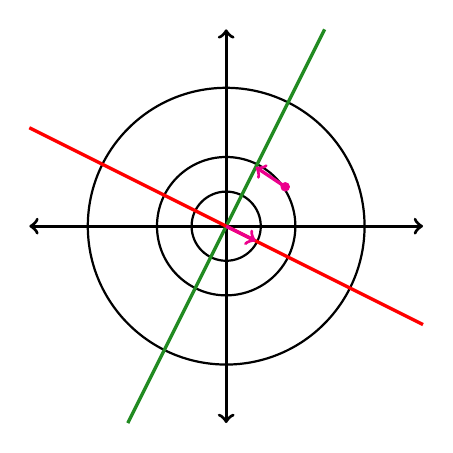
\begin{tikzpicture}[scale=0.25]
			\draw[black, thick] (0,0) circle(100pt);
			\draw[black, thick] (0,0) circle(200pt);
			\draw[black, thick] (0,0) circle(50pt);
			\draw[very thick,<->] (0,10)--(0,-10);
			\draw[very thick,<->] (10,0)--(-10,0);
			\draw[very thick, ForestGreen] (-5,-10)--(5,10);
			\draw[very thick, red] (-10,5)--(10,-5);
			\filldraw[magenta] (3,2) circle(6pt);
			\draw[magenta, very thick, ->] (3,2)--(1.5,3);
			\draw[magenta, very thick, ->] (0,0)--(1.5,-0.75);
		\end{tikzpicture}
		\caption{\textcolor{ForestGreen}{Column Space} and \textcolor{red}{Null Space} of $R$ in a simple example. An \textcolor{magenta}{element} is projected onto the column space, leaving residuals in the null space that are also standard normal.}
		\label{fig:overspecification_visualization}
	\end{figure}
\end{example}

\begin{definition}
	Let $\theta = r(\beta)$ and $\hat{\theta} = r(\hat{\beta})$ for some function $r: \reals^k \to \reals^q$, where $r \in \cont^1$. Suppose also that $R(\beta) = \frac{\partial r(\beta)}{\partial \beta'}$ has full rank of $q$ at the true value of $\beta$. Then we can construct a \blue{Wald test}:
	\[
	W \equiv n(\hat{\theta} - \theta)\parl R(\hat{\beta})' \hat{V}_\beta R(\hat{\beta})\parr^{-1} (\hat{\theta} - \theta) \todist \chi^2_q
	\]
	We will later develop other tests in a more general setting. 
\end{definition}


\begin{remark}
	We can extend this analysis to multiple equations, where 
	\begin{align*}
		Y_m &= X_m\beta_m + \varepsilon_m &&m = 1,\dots,M \\
		\expect Z_m \varepsilon_m &= 0 &&m=1,\dots,M
	\end{align*}
	The $X_m$ may be the same (like in seemingly unrelated regression equations), or they may overlap (like in panel data with some time invariant regressors) -- coefficients are not restricted across equations in a general setting, but they are in many applications.
\end{remark}

\begin{example}
	In \blue{Seemingly Unrelated Regressions} (this example from \href{https://www.jstor.org/stable/1831103?seq=1}{Griliches, 1976}), we may have that 
	\begin{align*}
		\textit{LW69} &= \alpha_1 + \beta_1 \cdot \textit{schooling69} + \gamma_1 \cdot \textit{IQ} + \delta_1 \cdot \textit{experience69} + \varepsilon_1 \\ \textit{KWW} &= \alpha_2 + \beta_2 \cdot  \textit{schooling69} + \gamma_2 \cdot \textit{IQ} + \varepsilon_2
	\end{align*}
	where \textit{LW69} is the logged wage, and \textit{KWW} is a measure of ability (as are \textit{IQ} and \textit{experience69}). We can think of this as regressing the two outcomes on the same regressor but assuming \emph{a priori} that $\delta_1 = 0$. That alone makes this model overidentified, and jointly estimating both equations leads to a more efficient estimate (\emph{if we believe the assumptions!}). We can construct a (fictitious) version of this with \blue{panel data}, and get
	\begin{align*}
		\textit{LW69} &= \alpha_1 + \beta_1 \cdot \textit{schooling69} + \gamma_1 \cdot \textit{IQ} + \delta_1 \cdot \textit{experience69} + \varepsilon_1 \\
		\textit{LW80} &= \alpha_2 + \beta_2 \cdot \textit{schooling80} + \gamma_2 \cdot \textit{IQ} + \delta_2 \cdot \textit{experience80} + \varepsilon_2
	\end{align*}
	We can define
	\begin{align*}
		\bar{Y} &= \matrixc{Y_1 \\ \vdots \\ Y_M} &&\bar{X} = \matrixc{X_1 & 0 & \cdots & 0 \\0 & X_2 & \cdots & 0 \\ \vdots & \vdots & \ddots & \vdots \\ 0 & 0 & \cdots & X_M} \\
		\bar{\beta} &= \matrixc{\beta_1 \\ \vdots \\ \beta_M} &&\bar{Z} = \;\matrixc{Z_1 & 0 & \cdots & 0 \\0 & Z_2 & \cdots & 0 \\ \vdots & \vdots & \ddots & \vdots \\ 0 & 0 & \cdots & Z_M} 
	\end{align*}
	and we have the moment condition \[\expect(\bar{Z}(\bar{Y}-\bar{X}'\bar{\beta})) = 0\]and estimator\[\hat{\beta}(W) = \parl\expect_n(\bar{X}\bar{Z}')W\expect_n(\bar{Z}\bar{X}')\parr^{-1}\parl\expect_n(\bar{X}\bar{Z}')W\expect_n(\bar{Z}\bar{Y})\parr\]The estimator is the same as before, except that the data matrix notation becomes unwieldy. Assuming that $(\bar{Y},\bar{X},\bar{Z})$ fulfill Assumptions~\ref{ass:gmm}, we have that 
	\begin{align*}
		\sqrt{n}(\hat{\beta}(W) - \beta) &\todist \normal(0,V_\beta)\\
		V_\beta &= (\bar{Q}'W\bar{Q})^{-1} \bar{Q}'W\bar{\Omega} W\bar{Q}(\bar{Q}'W\bar{Q})^{-1} \\
		\bar{Q} &= \expect(\bar{Z}\bar{X}') \\
		\bar{\Omega} &= \expect(\bar{Z} \varepsilon\varepsilon\bar{Z}')
	\end{align*}
	and results on efficient GMM are also the same as before.
\end{example}
	
	\begin{remark}
		This is extremely powerful! We just derived a collection of historically distinct estimators. A small caveat is that we must think very carefully about what the assumptions on the new objects actually mean. We've made the assumption that $(X_1,\dots,X_M,Y_1,\dots,Y_M,Z_1,\dots,Z_M)$ are \emph{all} i.i.d., which is stronger than assuming that equation-by-equation. 
	\end{remark}

\begin{remark}
	This is the same as estimating the equations separately (\ie will lead to the same result) if (i) everything is just identified \emph{or} (ii) $W$ is block diagonal, where its blocks correspond to equations. It can be instructive to write out the estimator for $M = 2$:
	\begin{align*}
		\hat{\beta}(\hat{W}) &= \barl \matrixc{\expect_n(X_1Z_1') & 0 \\ 0 & \expect_n(X_2Z_2')}\matrixc{W_{11} & W_{12} \\ W_{21} & W_{22}} \matrixc{\expect_n(X_1Z_1') & 0 \\ 0 & \expect_n(X_2Z_2')}\barr^{-1} \\
		&\;\quad \cdot \matrixc{\expect_n(X_1Z_1') & 0 \\ 0 & \expect_n(X_2Z_2')}\matrixc{W_{11} & W_{12} \\ W_{21} & W_{22}} \matrixc{\expect_n(Z_1Y_1) \\ \expect_n(Z_2Y_2)} \\
		&= \matrixc{\expect_n(X_1Z_1') W_{11} \expect_n(Z_1X_1') & \expect_n(X_1Z_1') W_{12} \expect_n(Z_2X_2') \\\expect_n(X_2Z_2') W_{21} \expect_n(Z_1X_1') & \expect_n(X_2Z_2') W_{22} \expect_n(Z_2X_2')} \cdot \matrixc{\expect_n(X_1Z_1') W_{11} \expect_n(Z_1Y_1) + \expect_n(X_1Z_1') W_{12} \expect_n(Z_2Y_2) \\ \expect_n(X_2Z_2') W_{21} \expect_n(Z_1Y_1) + \expect_n(X_2Z_2') W_{22} \expect_n(Z_2Y_2)} \\
		&\text{What happens if $W_{12} = W_{21} = 0$? We get the simplification:} \\
		&= \matrixc{\expect_n(X_1Z_1') W_{11} \expect_n(Z_1X_1') & 0 \\0& \expect_n(X_2Z_2') W_{22} \expect_n(Z_2X_2')} \cdot \matrixc{\expect_n(X_1Z_1') W_{11} \expect_n(Z_1Y_1)  \\  \expect_n(X_2Z_2') W_{22} \expect_n(Z_2Y_2)} \\
		&= \matrixc{(\expect_n(X_1Z_1') W_{11} \expect_n(Z_1X_1'))^{-1}\expect_n(X_1Z_1') W_{11} \expect_n(Z_1Y_1) \\ (\expect_n(X_2Z_2') W_{22} \expect_n(Z_2X_2'))^{-1}\expect_n(X_2Z_2') W_{22} \expect_n(Z_2Y_2)} \\
		&= \matrixc{\hat{\beta}_1(W_{11}) \\ \hat{\beta}_2(W_{22})}
	\end{align*}
	So when we assume that the cross-equation weights are zero, the multi-equation GMM just stacks the single equation estimators!
\end{remark}

\begin{question}
	When should we estimate equations jointly?
\end{question}
\begin{answer}
	If we naively interpret this result, we could estimate all of the equations in the world jointly -- if they're actually unrelated, the weighting matrix will pick that up. This seems intuitively untrue, but how do we show it formally? Well, we face an escalating number of nuisance parameters (entries of $W$). More importantly, model misspecification is contagious -- the estimator's probability limit equals \[\text{plim } \hat{\beta}(W) = \beta + \parl \expect(\bar{X}\bar{Z}')W\expect(\bar{Z}\bar{X}')\parr^{-1}\expect(\bar{X}\bar{Z}')W \expect(\bar{Z}\varepsilon)\]If any one entry of $\expect(\bar{Z}\varepsilon)$ is nonzero, then every entry of the matrix product is nonzero. This holds unless $W$ is block diagonal in the equations. In that case (and \emph{only} that case!) the joint estimation is efficient.
\end{answer}

\begin{example}
	\red{Multiple Regression vs. Seemingly Unrelated Regression} If $X_1 = \cdots = X_M = Z_1 = \cdots = Z_M$, then this is just multiple regression -- that is, we regress different $Y_1,\dots,Y_M$ on the same exogenous regressors. We can verify that the estimator just stacks OLS in this case.
	
	Alternatively, suppose that some regressors are dropped from some equations, meaning that we think their coefficients are zero. However, we still consider them exogenous in all equations, so we can use them as overidentifying instruments. Formally, let $Z_1 = \cdots = Z_M = \bigcup_{m=1}^M X_m$ and the $X_m$ are not all the same. This is the \blue{Seemingly Unrelated Regression (SUR)} estimator.\footnote{Historically, it would also require homoskedasticity, but that's actually a distinct issue.}
\end{example}

\begin{remark}
	As we add assumptions to the basic model, we can recover some classic estimators that were developed independently. These assumptions typically allow us to simplify expressions. See Hayashi for more detail.
	\begin{itemize}
		\item If we assume homoskedasticity, we get \blue{Full Information Instrumental Variables Efficient (FIVE) estimation} (from \href{https://www.jstor.org/stable/1937965}{Brundy \& Jorgenson, 1971})
		\item If we additionally assume that $Z_1 = \cdots = Z_M$, we get \blue{Three-Stage Least Squares (3SLS)}\footnote{In modern terminology, this is a two-stage estimator. However, it could be expressed as TSLS with `pre-pre-estimation' of cross-equation correlation of errors, hence the name.} (from \href{https://www.jstor.org/stable/1911287}{Zellner \& Theil, 1962})
		\item SUR is the final specialization, where we set $Z_1 = \cdots = Z_M = \bigcup_{m=1}^M X_m$
	\end{itemize}
\end{remark}

\begin{remark}
	Next, we can think about common coefficients. Consider the following specification: \[Y_m = X_m \beta + \varepsilon_m,\qquad \expect Z_m \varepsilon_m = 0 \forall m = 1,\dots,M\]The main intuition here is that an essentially the same (but not constant) covariate is observed across equations. We do not need to revisit every covariate in every equation: some components of $X_m$ could be zero almost surely. If we define \[\bar{Y}= \matrixc{Y_1 \\ \vdots \\Y_M}\quad ; \quad \bar{X} = \matrixc{X_1 & \cdots & X_M} \quad ; \quad \bar{Z} = \matrixc{Z_1 & 0 & \cdots & 0 \\ 0 & Z_2 & \cdots & 0 \\ \vdots & \vdots &\ddots &\vdots \\ 0 & 0 & \cdots & Z_M}\]then we have moment condition $\expect(\bar{Z}(\bar{Y} - \bar{X}'\beta)) = 0$ and estimator\[\hat{\beta}(W) = \parl \expect_n(\bar{X}\bar{Z}') W\expect_n(\bar{Z}\bar{X}')\parr^{-1}\expect_n(\bar{X}\bar{Z}') W\expect_n(\bar{Z}\bar{Y})\]This looks like what we had before, but the different definition of $\bar{X}$ changes identification: that $\expect(\bar{Z}\bar{X}')$ has full rank is implied by $\expect(Z_mX_m')$ having full rank for each $m= 1,\dots,M$.
	
	Common coefficients allow for estimation of many parameters that would not otherwise be identifiable. An important application is panel data:
	\begin{itemize}
		\item If we impose the assumptions that characterized SUR before, we get the \blue{Random Effects} estimator
		\item If we furthermore assume that $\varepsilon_m$ is uncorrelated across $m$, then this simplifies to \blue{Pooled OLS}
	\end{itemize}
	The difference between those estimators is about efficiency, not identification. We will revisit random effects and pooled OLS soon.
\end{remark}

\begin{remark}
	Efficient GMM vaguely resembles WLS or \blue{Feasible Generalized Least Squares (FGLS)}. As a reminder, weighted least squares minimizes \[(Y - X\beta)' W(W-X\beta)\]where the weighting matrix $W$ gives differential weights to different observations. If we know that $\expect(\varepsilon\varepsilon' \mid X) = \sigma^2 \cdot \Omega$ for known $\Omega$, then setting $W = \Omega^{-1}$ is variance minimizing, and the resulting estimator is the BLUE by Gauss-Markov. To see the analogy to WLS as undergraduates learn it, note that we can equivalently minimize \[(C(Y-X\beta))'(C(Y-X\beta))\]where $C$ is the Cholesky root of $W$. In particular, if observations are uncorrelated, \[\Omega = \matrixc{\sigma_1^2 & 0 & \cdots & 0 \\ 0 & \sigma_2^2 & \cdots & 0 \\ \vdots & \vdots &\ddots & \vdots \\ 0 & 0 & \cdots & \sigma_n^2}\quad ; \quad \Omega^{-1} = \matrixc{1/\sigma_1^2 & 0 & \cdots & 0 \\ 0 & 1/\sigma_2^2 & \cdots & 0 \\ \vdots & \vdots &\ddots & \vdots \\ 0 & 0 & \cdots & 1/\sigma_n^2}\quad ; \quad C =  \matrixc{1/\sigma_1 & 0 & \cdots & 0 \\ 0 & 1/\sigma_2 & \cdots & 0 \\ \vdots & \vdots &\ddots & \vdots \\ 0 & 0 & \cdots & 1/\sigma_n}\]and the minimand can be expressed as $\sum_{i=1}^n ((y_i - x_i'\beta) / \sigma_i)^2$. 
	\end{remark}
	\begin{question}
		What do we do if we don't know $\Omega$? We could estimate it, but estimating an $n \times n$ matrix from $n$ data points seems absurd. 
	\end{question}
	There's two possible paths: (i) if we have a specific parameter model for how $\expect(\varepsilon^2 \mid X = x)$ changes with $x$, we could estimate it; and (ii) we could run a general flexible regression of $\hat{\mu}_i^2$ on $X$. The latter regressions are often run to construct Breusch-Pagan or other heteroskedasticity tests. However, (i) is rare and for (ii) we incur a lot of effort (and error propogation!) for reweighting that only matters if weights are very different than even. This explains why the latter approach has a name (Feasible Generalized Least Squares) but is extremely uncommon in practice.
	
	So what does this have to do with GMM? We can write the GMM estimator as the weighted OLS estimator in a fictitious regression, where we set $\mu = Z'Y$ and $G = Z'X$, then we want to minimize \[(\mu - G\beta)'W(\mu - G\beta)\]and this looks like WLS with $k$ regressors, $\ell$ observations, and weight matrix $W$. The closed-form WLS estimator\[\hat{\beta}_{WLS} = (G'WG)^{-1} G'W\mu\]precisely recovers the GMM estimator (once we substitute back the transformations). So if GMM is similar to FGLS, why is it so much more common?  The analogy is useful but has limitations. Every moment condition in the original problem is an `observation' in the fictitious regression. In our WLS analogy, the `error' is $\eta \equiv \mu - G\beta$, with variance-covariance matrix of size $\ell \times \ell$, so we are estimating a much smaller matrix, which becomes a lot more precise as $n$ grows! We can also see this in the objective functions:
	\[
	(Y-X\beta)' \underbrace{W}_{n \times n}(Y - X\beta) \qquad\qquad \text{ vs. } \qquad\qquad (\mu - G\beta)'\underbrace{W}_{\ell \times \ell} (\mu - G\beta)
	\]


\newpage
\section{Panel Data}

\begin{remark}
	An \emph{extremely quick} and non-exhaustive treatment.
\end{remark}

\begin{definition}
	\blue{Panel data} are data that come in a two-dimensional array, most commonly in `time' and `units of observation'. We have \blue{sample size} $n$ and \blue{number of waves} $T$. With a \blue{balanced panel}, we have $nT$ observations.\footnote{We will consider only balanced panels.} We call a \blue{short panel} one where in practice $T \ll n$, and the asymptotics require that we fix $T$ and let $n \to \infty$. Alternatively, we have a \blue{long panel}, where we fix $n$ and let $T \to \infty$. This is really a multivariate time series. Some applications require analyses where we send $n\to\infty$ and $T \to\infty$ at the same or different rates. Here, we consider only short panels.
\end{definition}

\begin{remark}
	All estimators in this section are variations on multiple equation common coefficients GMM. We will develop from specific to general here, starting with \[Y_{it} = X_{it}'\beta + \varepsilon_{it} \qquad \text{ where } \expect(X_{it}\varepsilon_{it}) = 0\]From there, we get:
\end{remark}
\begin{definition}
	The \blue{pooled OLS estimator} is defined as \[\hat{\beta}_{pool} \equiv \parl \sum_{i=1}^n X_i'X_i\parr^{-1} \sum_{i=1}^n X_i'Y_i = (X'X)^{-1}X'Y \toprob \beta\]This is unbiased and consistent under the assumptions that confirm that previously (where $X$ and $Y$ are pooled data matrices). It also has the same asymptotics if we make the same assumptions as above. However, the homoskedasticity assumption is \emph{incredibly} strong here. At the very least, we need to use a \blue{cluster-robust variance estimator}\[\hat{V}_{pool} = (X'X)^{-1} \parl \sum_{i=1}^n X_i' \hat{\varepsilon}_i\hat{\varepsilon}_i X_i\parr (X'X)^{-1}\]We had previously omitted cluster-dependent errors, but note the analogy to FGLS: the central term estimates the $(T \times T)$-matrix $\expect(X_i'\hat{\varepsilon}_i\hat{\varepsilon}_i X_i)$. However, we could do even better! As previously, the variance matrix is `small', which raises the possibility of using an FGLS-like approach for estimation. In fact, we are precisely doing efficient (multi-equation) GMM. 
\end{definition}

\begin{definition}
	A popular model is the \blue{Random Effects Model}, where we assume cross-sectional homoskedasticity but with the specific structure \[\expect(\varepsilon_i\varepsilon_i' \mid X_i) = \matrixc{\sigma_u^2 + \sigma_\epsilon^2 & \sigma_u^2 & \cdots & \sigma_u^2 \\ \sigma_u^2 & \sigma_u^2 + \sigma_\epsilon^2 & \cdots & \sigma_u^2 \\\vdots & \vdots & \ddots & \vdots \\ \sigma_u^2 & \sigma_u^2 & \cdots & \sigma_u^2 + \sigma_\epsilon^2}\]which has only two degrees of freedom. The assumption here is that $\varepsilon_{it} = u_i + \epsilon_{it}$ where $u_i$ and $\epsilon_{it}$ are uncorrelated. In other words, our structural equation becomes the model \[Y_{it} = X'_{it} \beta + u_i + \epsilon_{it} \text{ where } \expect(X_{it}u_i) = \expect(X_{it}\epsilon_{it}) = 0\]
\end{definition}
\begin{remark}
	The random effects estimator can be thought of as the feasible GLS estimator for this model, where we pre-estimate $\sigma_u$ and $\sigma_\epsilon$. We will get more details later, under some theory yet to come. Note that Hayashi defines the random effects estimator as a two-stage GMM assuming homoskedasticity, which is similar to three-stage least squares. This treatment has more degrees of freedom.  
\end{remark}
What's important is that (i) random effects has the same identifying assumptions as pooled OLS, and (ii) it adds a FGLS/TSGMM step, and since within-unit correlation of $\varepsilon$ is both salient and easily modeled (note: in short panels only!), this is often desirable.

\begin{remark}
	In the random effects model, the condition that $\expect X_{it}u_i = 0$ is very restrictive. If we think of $u_i$ as unobserved, time-invariant covariates, we are saying that these cannot at all be correlated with the observed. If this fails, do we have anything else to estimate?
	
	Consider the \blue{Fixed Effects (FE)} equation \[Y_{it} - Y_{i,t-1} = (X_{it} - X_{i,t-1})'\beta + \epsilon_{it} - \epsilon_{i,t-1}\]
	When can we estimate this by OLS? We need that (i) $\epsilon_{it}$ is uncorrelated with past and future $\epsilon_{t}$, and (ii) that $(X_{it} - X_{i,t-1})$ fulfills a rank condition (this will fail with time-invariant regressors). This is the basic idea of fixed effects estimation, where we can `difference away' the fixed effects in one of three ways: (i) first differencing (\blue{between estimator}), (ii) demeaning (\blue{within estimator}), and (iii) adding an indicator of each unit (\blue{dummy variable regression}). Demeaning and dummy variables are numerically the same, and correspond to the `classic' fixed effects estimator. From the point of view of identification, the methods are the same, but they imply different weighting matrices. If the weighting matrix is pre-estimated, they are asymptotically the same.
	
	We additionally have that:
	\begin{enumerate}
		\item The implied weighting matrix $M = 1 (1'1)^{-1}1'$ is efficient if the idiosyncratic error $\epsilon_{it}$ is homoskedastic and uncorrelated. (for the between estimator, we need that $\epsilon_{it}$ follows a random walk in direction $t$. This is less salient)
		\item We can actually show that FE equals TSLS (or really SUR), thinking of the cross-equation restrictions in \[\expect X_{is} \epsilon_{it} = 0 \forall s,t\]as overidentifying restrictions / instruments
		\item The estimator necessarily has higher (asymptotic) variance than pooled OLS. This is because OLS algebra applies, but demeaning reduces the sum of squared deviations of any random variable
		\item For variance estimation, a degrees of freedom adjustment of $T(T-1)$ is not negligible for realistic $T$ and is therefore recommended for including under asymptotic justification
		\item In the formal model that motivates the random effects model, the FE estimator can be used to estimate $\sigma_\epsilon^2$. Doing this first and then backing out $\sigma^2_u$ is the standard approach
	\end{enumerate}
	
	\begin{assumption}\label{ass:fe_panel}
		We assume the following:
		\begin{enumerate}
			\item $Y_{it} = X_{it}' + u_i + \epsilon_{it}$ for all $t = 1,\dots,T$, $T \ge 2$
			\item $X_{it}$ are i.i.d.
			\item $\expect(X_{is}\epsilon_{it}) = 0$ for all $s,t = 1,\dots,T$
			\item $Q \equiv \expect(\bar{X}_i',\bar{X}_i)$ is positive definite, where $\bar{X}_i = (X_{i2} - \bar{X}_i,\dots,X_{it} - \bar{X}_i)'$
			\item $\expect\epsilon_{it}^4 < \infty$, $\expect \|X_{it}\|^4 < \infty$
		\end{enumerate}
	\end{assumption}
	\begin{theorem}
		Under Assumptions~\ref{ass:fe_panel}, \begin{align*} \sqrt{n}(\hat{\beta}_{\textnormal{fe}} - \beta) &\todist \normal(0,Q^{-1}\Omega Q^{-1}) \\Q &\equiv \expect(\bar{X}_i' \epsilon_i\epsilon_i' \bar{X}_i)\end{align*}
	\end{theorem}
\end{remark}

\begin{remark}
	Though we don't go into it here, it is true that undetrended time series can exhibit extreme (and considerably confounded) correlations. This motivates us to detrend our panel and estimate the equation \[Y_{it} = X_{it} \beta + u_i + \nu_t + \epsilon_{it}\]This is called the \blue{Two-Way Fixed Effects (TWFE)} model, and when $T = 2$ (only!) it is equivalent to the \blue{difference-in-difference (DiD)} estimation. The best known estimator is the pooled OLS after a double-within transformation. This is the subject of an active literature (see: \href{https://www.sciencedirect.com/science/article/pii/S0304407620303948}{Callaway \& Sant'Anna (2021)}, \href{https://file-lianxh.oss-cn-shenzhen.aliyuncs.com/Refs/XuDID/Goodman-Bacon-2021-JoE.pdf}{Goodman-Bacon (2021)}, etc) and you should consult with an econometrician before using it.
\end{remark}



\begin{definition}
	The \blue{dynamic panel} is estimated by the equation \[Y_{it} = \alpha\cdot Y_{i,t-1} + X_{it}\cdot \beta + u_i + \epsilon_{it}\]We consider only one lag for exposition. In practice if data have a trend it would be essential to separately model that to avoid spurious correlation. The qualitatively new problem is that, even under the preceding assumptions, we have that $Y_{it}$ is an endogenous regressor in the transformed data. It is most easily seen with first differencing:\[\expect(\Delta Y_{i2} \Delta \epsilon_{i3})= \expect((Y_{i2} - Y_{i1})(\epsilon_{i3} - \epsilon_{i2})) = \underbrace{\expect(Y_{i2}\epsilon_{i3})}_{0} - \underbrace{\expect(Y_{i1}\epsilon_{i3})}_{0} - \underbrace{\expect(Y_{i2}\epsilon_{i2})}_{\sigma^2_\epsilon} + \underbrace{\expect(Y_{i1}\epsilon_{i2})}_{0} = -\sigma^2_\epsilon\]This finding implies that FE estimation is biased and inconsistent. In fact, if we assume stationarity ($|\alpha|<1$), the asymptotic bias of $\hat{\alpha}$ can be computed as \[\text{plim } \hat{\alpha}_{\text{fe}} = \alpha - \frac{1+\alpha}{2\alpha / (1-\alpha) + (T-1)/(1-\alpha^{T-1})}\]and a bias of the same order (\ie $O(1/T)$) is inherited by $\hat{\beta}$. Note that the bias is negative and not particularly small even for moderately large $T$. We can conclude that FE are not appropriate in this setting. The previous is from \href{https://www.jstor.org/stable/1911408}{Nickell (1981)} and is often called the \blue{Nickell Critique}. Some practitioners deliberately ignore this because the fixes have their own issues.
\end{definition}

\begin{remark}
	What can we do about this? Instrumental variables! We write that \[\cov(Y_{i,t-2},\Delta Y_{i,t-1}) \ne 0 \qquad ; \qquad \expect(Y_{i,t-1}\Delta \epsilon_{it}) = \expect(Y_{i,t-2}\epsilon_{it}) - \expect(Y_{i,t-2}\epsilon_{i,t-1}) = 0\]So as long as $T \ge 3$, we have an instrument. (More generally, $T$ must exceed the number of lags of $Y$ used by at least 2). This gives rise to the \blue{(Anderson-)Hsiao Estimator}. An important limitation is that the estimator is very sensitive to misspecification, meaning that $\epsilon_{it}$ must actually be uncorrelated and the correct number of lags must be specified. The above algebra also implies that $Y_{i,t-3}, Y_{i,t-4},\dots$ are valid and relevant instruments (though they get weaker with distance). We can also do overidentified multiple GMM, which is the \blue{Arellano-Bond Estimator}, which exists as a one-step (as in TSLS) or a two-step (as in Efficient GMM) estimator.
\end{remark}


\section{Extremum Estimation}

\begin{definition}
	An \blue{extremum estimator} is any estimator defined as \[\hat{\theta} = \argmin_{\theta\in\Theta} Q_n(W_1,\dots,W_n;\theta)\]for some parameter $\theta$ in parameter space $\Theta$, where $W_1,\dots,W_n$ is a sample. The \blue{criterion function} $Q_n(\cdot)$ must be indexed by $n$ because its mathematical form necessarily depends on $n$. However, usually it is intuitively the same function at different $n$. Consider for example $Q_n(\cdot) = \frac{1}{n}\sum_{i=1}^n (Y_i - X_i'b)^2$. Similarly to GMM notation, we will often drop the data and call this $Q_n(\theta)$.
\end{definition}
\begin{remark}
	The intuition for why this would estimate a true parameter value $\theta_0$ is that:
	\begin{align*}
		\theta_0 &= \argmin_{\theta\in\Theta} Q(\theta) &&\hat{\theta} = \argmin_{\theta\in\Theta} Q_n(\theta) \\ Q_n(\cdot) &\to Q(\cdot) \qquad \qquad \qquad \qquad \qquad\overset{?}{\Longrightarrow} &&\hat{\theta} \to \theta_0
	\end{align*}
	That is, the \blue{sample criterion} $Q_n(\cdot)$ estimates some \blue{population criterion} $Q(\cdot)$ that is minimized at $\theta_0$. Intuitively, in `nice' cases that implies that $\hat{\theta} \to \theta_0$. An illustration of a `nice' case is Figure~\ref{fig:extremum_estimation}.
	
	\begin{figure}[H]
	\centering
		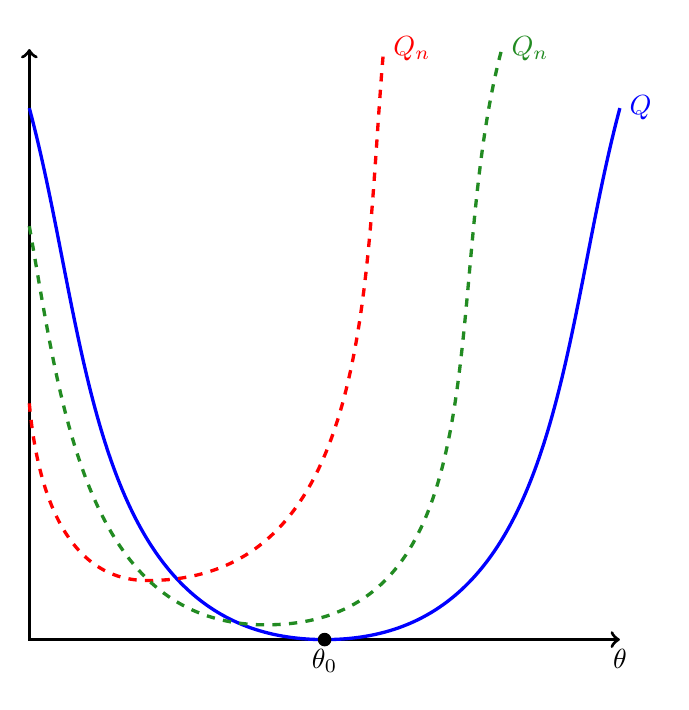
\begin{tikzpicture}[scale = 0.75]
			\draw[<->,very thick] (0,10)--(0,0)--(10,0);
			\node[below] at (10,0) {$\theta$};
			\draw[very thick, blue] (0,9) to[out=-75,in=180] (5,0) to[out=0,in=-105] (10,9);
			\node[right] at (10,9) {\textcolor{blue}{$Q$}};
			\draw[very thick, red, dashed] (0,4) to[out=-85,in=180](2,1)to[out=0,in=-95](6,10);
			\node[right] at (6,10) {\textcolor{red}{$Q_n$}};
			\draw[very thick, ForestGreen, dashed] (0,7) to[out=-80,in=180](4,0.25)to[out=0,in=-105](8,10);
			\node[right] at (8,10) {\textcolor{ForestGreen}{$Q_n$}};
			\filldraw (5,0) circle(3pt);
			\node[below] at (5,0) {$\theta_0$};
		\end{tikzpicture}
		\caption{`Nice' Extremum Estimation, with the \textcolor{blue}{true criterion function}, an estimate with \textcolor{red}{small $n$}, and an estimate with \textcolor{ForestGreen}{larger $n$}. The true $\theta_0$ is additionally marked.}.
		\label{fig:extremum_estimation}
	\end{figure}
\end{remark}

\begin{example}
	\red{GMM}\begin{align*}
		Q(\theta) &= \expect g(\theta)' W \expect g(\theta) \\
		Q_n(\theta) &= \expect_n g(\theta)' \hat{W} \expect_n g(\theta)
	\end{align*}
\end{example}
\begin{example}
	\red{Method of Simulated Moments (MSM)}
	\begin{align*}
		Q(\theta) &= (\pi(\theta) - \pi_0)' W (\pi(\theta) - \pi_0) \\
		Q_n(\theta) &= (\tilde{\pi}(\theta) - \hat{\pi})' \hat{W} (\tilde{\pi}(\theta) - \hat{\pi})
	\end{align*}
	The function $\pi(\cdot)$ maps parameter values onto implies moments of the data (\eg means, variances, or even entire time series of inflation, unemployment, etc...), where $\pi_0$ are the true moments and $\hat{\pi}$ an estimate, and $\tilde{\pi}(\cdot)$ is a \blue{simulated analog} of $\pi(\cdot)$. This (interestingly) differs from GMM if simulation noise in $\tilde{\pi}(\cdot)$ cannot be ignored. Otherwise, it is just GMM (but sometimes called MSM).
\end{example}

\begin{example}
	\red{Nonlinear Least Squares}
	\begin{align*}
		Q(\theta) &= \expect (Y - m(X,\theta))^2 \\
		Q_n(\theta) &= \expect_n (Y - m(X,\theta))^2 
	\end{align*}
	You could argue that this an example of GMM (and it is!) but it was developed separately.
\end{example}
\begin{example}
	\red{Maximum Likelihood}
	\begin{align*}
		Q(\theta) &= \expect \ell(W;\theta) \\
		Q_n(\theta) &= \expect_n \ell(W;\theta)
	\end{align*}
	The ``conceptual'' definition is at first glance different, but we will later derive the above from it.
\end{example}

\begin{definition}
	The most important special case are \blue{$m$-estimators}, where \begin{align*}
		Q(\theta) &= \expect m(W;\theta) \\ Q_n(\theta) &= \expect_n m(W;\theta)
	\end{align*}
	for some known, real-valued function $m(\cdot)$. Some examples are maximum likelihood, where $m(W;\theta) = \ell(W;\theta)$, and one-step GMM where $m(W;\theta) = g(W;\theta)' W g(W;\theta)$. Consider why efficient GMM is not an $m$-estimator. This class of estimators is of interest because some of the building blocks of asymptotic theory are available at exactly this level of geometry. Note that some texts (\emph{not} Hayashi) use $m$-estimation as a synonym for extremum estimation.
\end{definition}

\begin{remark}
	We will next formalize the intuitive argument for consistency. We will start at a high-level and then verify in special cases. The following will assume that $\argmin_{\theta\in\Theta} Q_n(\theta)$ exists, and we could see that everything goes through as long as $Q_n(\hat{\theta}) \le \inf_{\theta\in\Theta} Q_n(\theta) + \frac{1}{n}$. Thus, $\hat{\theta}$ can be an arbitrary choice that fulfills this constraint. This settles existence and is also practically relevant because $\hat{\theta}$ may be numerically evaluated and thus not exact. 
\end{remark}

\begin{theorem} \red{Consistency}
	Assume that:
	\begin{enumerate}
		\item The sample criterion uniformly consistently estimates the population criterion: \[\sup_{\theta\in\Theta} |Q_n(\theta) - Q(\theta) | \toprob 0\]
		\item $\theta_0$ is a unique and well-separated global minimum of $Q(\cdot)$: \[\forall \varepsilon > 0, \exists \delta > 0 \st Q^\varepsilon \equiv \inf_{\theta \in \Theta : \|\theta - \theta_0\|\ge \varepsilon} Q(\theta) \ge Q(\theta_0) + \delta\]
	\end{enumerate}
	Then $\hat{\theta} \toprob \theta_0$.
\end{theorem}
\begin{proof}
	Fix $\varepsilon > 0$ and define $Q_n^\varepsilon \equiv \inf_{\theta \in \Theta : \|\theta - \theta_0\| \ge \varepsilon} Q_n(\theta)$. Then we have that \begin{align*} \prob \parl \|\hat{\theta} - \theta_0\| > \varepsilon \parr &\le \prob\parl Q_n^\varepsilon \le Q_n(\theta_0)\parr \\ &= 1 - \prob \parl Q_n^\varepsilon > Q_n(\theta_0)\parr \\ &\le 1 - \prob\parl Q_n^\varepsilon > Q_\varepsilon - \frac{\delta}{2},Q_n(\theta_0) < Q(\theta_0) + \frac{\delta}{2}\parr \\ &\to 0 \end{align*} where all inequalities follow from logical implication, and the last step uses the first assumption. Thus, $\hat{\theta} \toprob \theta_0$.
\end{proof}

\begin{remark}
	The preceding result used both (i) uniform convergence and (ii) the well-separated minimum. We will provide lower-level conditions that imply these.
\end{remark}

\begin{theorem}
	If we assume that:
	\begin{enumerate}
		\item $Q(\cdot)$ is continuous
		\item $\Theta$ is compact
		\item $\theta_0 = \argmin_{\theta' \in \Theta} Q(\theta')$ is unique
	\end{enumerate}
	Then $\theta_0$ is a well-separated minimum.
\end{theorem}
\begin{proof}
	Fix $\varepsilon > 0$. By the Weierstrass Theorem, $Q^\varepsilon$ is attained by some $\theta^\varepsilon$ with $\|\theta^\varepsilon - \theta_0\| \ge \varepsilon$. Set $\delta = Q(\theta^\varepsilon) - Q(\theta_0)$, which is strictly positive by the third assumption.
\end{proof}


\begin{theorem}
	If we assume that:
	\begin{enumerate}
		\item $\hat{\theta}$ is an $m$-estimator
		\item The data are i.i.d. realizations of $W$
		\item $m(W;\theta)$ is almost surely continuous in $\theta$
		\item $|m(W;\theta)| \le G(W)$ for some function $G$ where $\expect G(W) < \infty$
		\item $\Theta$ is compact 
	\end{enumerate}
	then $Q_n(\cdot)$ converges to $Q(\cdot)$ uniformly.
\end{theorem}
\begin{proof}
	This is the \blue{Uniform Law of Large Numbers}.
\end{proof}

\begin{remark}
	We can consolidate the above into a single result:
\end{remark}

\begin{theorem}
	\red{Consolidated Consistency} Assume that
	\begin{enumerate}
		\item $Q(\cdot)$ is continuous
		\item $\Theta$ is compact
		\item $\theta_0$ uniquely minimizes $Q(\theta)$
		\item $\sup_{\theta\in\Theta} |Q_n(\theta) - Q(\theta)| \toprob 0$
	\end{enumerate}
	Then $\hat{\theta} \toprob \theta_0$.
\end{theorem}
\begin{proof}
	Sufficiency proved already. We can think intuitively about why each condition is necessary:
	
	\begin{enumerate}
		\item Continuity: Without continuity, we could have a unique but not well-separated minimum, so the function could be arbitrarily close while the estimate is far away.
		\item Compactness: If the minimizer is at the boundary of an open set (\ie a non-compact domain), then we will not approximate it, even with an arbitrarily good functional approximation! Alternatively, if the set is unbounded we could think of similar.
		\item Uniqueness: If $\theta_0$ is not unique, even a function that is a very good approximation of $Q$ may be minimized close to the `wrong' minimizer, as was seen when we thought about well-separated minima.
		\item Uniform Convergence: Consider converging pointwise rather than uniformly. We could very possibly have $Q_n$ limiting pointwise to a function with a true population minimum that is positive distance from any intermediate minima of the various $Q_n$. Think of the limiting behavior in Figure~\ref{fig:pointwise_conv}, where we have that the intermediate minima for each $Q_n$ are approaching the origin, while the population minimum is strictly positive.
	\end{enumerate}
\end{proof}
\begin{figure}[ht]
	\centering
	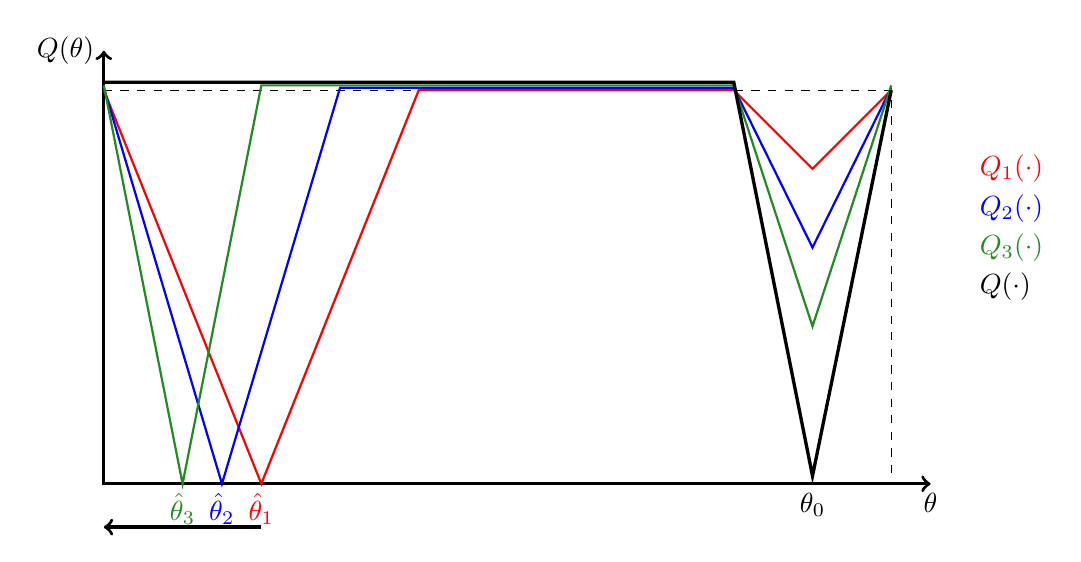
\begin{tikzpicture}
		\draw[very thick,<->] (0,5.5)--(0,0)--(10.5,0);
		\node[below] at (10.5,0) {$\theta$};
		\node[left] at (0,5.5) {$Q(\theta)$};
		\draw[dashed] (0,5)--(10,5)--(10,0);
		
		\draw[red, thick] (0,5)--(2,0)--(4,5)--(8,5)--(9,4)--(10,5);
		\draw[blue,thick] (0,5.03)--(1.5,0)--(3,5.03)--(8,5.03)--(9,3)--(10,5.03);
		\draw[ForestGreen, thick] (0,5.06)--(1,0)--(2,5.06)--(8,5.06)--(9,2)--(10,5.06);
		\draw[very thick] (0,5.1)--(8,5.1)--(9,0.1)--(10,5);
		
		\node[right] at (11,4) {\textcolor{red}{$Q_1(\cdot)$}};
		\node[right] at (11,3.5) {\textcolor{blue}{$Q_2(\cdot)$}};
		\node[right] at (11,3) {\textcolor{ForestGreen}{$Q_3(\cdot)$}};
		\node[right] at (11,2.5) {\bm{$Q(\cdot)$}};
		\node[below] at (9,0) {\bm{$\theta_0$}};
		\node[below] at (2,0) {\textcolor{red}{$\hat{\theta}_1$}};
		\node[below] at (1.5,0) {\textcolor{blue}{$\hat{\theta}_2$}};
		\node[below] at (1,0) {\textcolor{ForestGreen}{$\hat{\theta}_3$}};
		\draw[very thick, ->] (2,-0.55)--(0,-0.55);
	\end{tikzpicture}
	\caption{Pointwise (but not uniform) Convergence}
	\label{fig:pointwise_conv}
\end{figure}
\begin{remark}
	When $\theta_0$ is not unique, we could think of working with \blue{partial identification}, which involves estimation and inference theory for $\Theta_I = \argmin_{\theta\in\Theta} Q(\theta)$ (a possibly non-singleton \blue{identified set}). This is an active literature.
\end{remark}


\begin{theorem}
	\red{Consistency for Convex $Q(\cdot)$} If we assume that 
	\begin{enumerate}
		\item $\Theta$ is convex
		\item $\theta_0 \in \interior \Theta$
		\item $\theta_0$ uniquely minimizes $Q(\theta)$
		\item $Q_n(\cdot)$ is convex
		\item $|Q_n(\theta) - Q(\theta)| \toprob 0 \forall \theta \in \Theta$
	\end{enumerate}
	Then $\hat{\theta} \toprob \theta_0$.
\end{theorem}
\begin{proof}
	The proof of a simplified statement is left as homework. Essentially, we need only pointwise convergence, and the assumptions guarantee that there exists $\hat{\theta}$ that exactly minimizes $Q_n(\cdot)$.
\end{proof}


\begin{remark}
	We are abput to move on to $\sqrt{n}$-asymptotic normality. Are there intermediate assumptions under which we can ensure a rate of convergence without ensuring asymptotic normality? Yes! They relate the curvature of $Q(\cdot)$ at $\theta_0$ to that rate. The rate is $\sqrt{n}$ if $Q(\cdot)$ locally dominates some quadratic function. The proof is van der Vaart \& Wellner's \blue{Argmax Theorem} in \href{https://link.springer.com/book/10.1007/978-1-4757-2545-2}{Weak Convergence and Empirical Processes}.
\end{remark}


\begin{assumption}\label{ass:asymptotics_extremum}
	In order to obtain asymptotics, we need:
	\begin{enumerate}
		\item $\hat{\theta}\toprob \theta_0$
		\item $\theta_0 \in \interior(\Theta)$
		\item $Q_n(\cdot)$ is twice continuously differentiable in an open neighborhood $N$ of $\theta_0$
		\item $\sqrt{n}\frac{\partial Q_n(\theta_0)}{\partial \theta} \todist \normal(0,\Sigma)$
		\item $\sup_{\theta\in N} \Big\|\frac{\partial Q_n(\theta)^2}{\partial \theta \partial \theta'} - \frac{\partial Q(\theta)^2}{\partial \theta \partial \theta'}\Big\| \toprob 0$
		\item $\mathcal{H} \equiv \frac{\partial Q(\theta_0)^2}{\partial \theta \partial \theta'}  $ is nonsingular
	\end{enumerate}
\end{assumption}

\begin{theorem}
	\red{Extremum Estimation Asymptotics} Under Assumptions~\ref{ass:asymptotics_extremum}, \[\sqrt{n}(\hat{\theta} - \theta_0) \todist \normal(0,\mathcal{H}^{-1} \Sigma \mathcal{H}^{-1})\]
\end{theorem}
\begin{proof}
	By the definition of $\hat{\theta}$ and the first two assumptions, we have that almost surely\[\frac{\partial Q_n(\hat{\theta})}{\partial \theta} = 0\]Using the third assumption and the Mean Value Theorem, we get\[\frac{\partial Q_n(\hat{\theta})}{\partial \theta} = \frac{\partial Q_n(\theta_0)}{\partial \theta} + \frac{\partial Q_n(\bar{\theta})^2}{\partial \theta \partial \theta'}(\hat{\theta} - \theta_0)\]where $\bar{\theta}$ is coordinate-wise between $\hat{\theta}$ and $\theta_0$, in particular $\bar{\theta} \toprob \theta_0$. From here, we can combine to rearrange and we want to show that:\[\sqrt{n}(\hat{\theta} - \theta_0) = \underbrace{-\parl \frac{\partial Q_n(\bar{\theta})^2}{\partial\theta\partial \theta'}\parr^{-1}}_{\toprob \mathcal{H}^{-1}} \underbrace{\sqrt{n}\frac{\partial Q_n(\theta_0)}{\partial \theta}}_{\todist \normal(0,\Sigma)}\]The only thing left to show is the convergence to $\mathcal{H}$. To keep everything neat, define $H(\theta) = \frac{\partial Q(\theta)^2}{\partial \theta \partial \theta'}$ and $H_n(\cdot)$ analogously. Then we have that 
	\begin{align*}
		\big\|H_n(\bar{\theta}) - \mathcal{H}\big\| &= \big\| H_n(\bar{\theta}) - H(\bar{\theta}) + H(\bar{\theta}) - \mathcal{H}\big\| \\
		(\text{by } \triangle)\;\; &\le \big\| H_n(\bar{\theta}) - H(\bar{\theta})\big\| + \big\|H(\bar{\theta}) - \mathcal{H}\big\| \\
		(\text{by Assumption 1})\;\; &\le \sup_{\theta\in N} \big\| H_n(\theta) - H(\theta)\big\| + \big\|H(\bar{\theta}) - \mathcal{H}\big\| \\
		(\text{by Assumptions 3 \& 5})\;\; &\toprob 0
	\end{align*}
	The claim now follows directly from nonsingularity of $\mathcal{H}$ and Continuous Mapping Theorem.
\end{proof}

\begin{remark}
	We can slightly improve on this if the application is specifically nonlinear GMM. Recall that $\hat{\theta} = \argmin_{\theta\in\Theta} \{\bar{g}_n(\theta)' W \bar{g}_n(\theta)\}$.
\end{remark}

\begin{assumption}\label{ass:asymptotics_nonlinear_gmm}
	We slightly refine the above assumptions to fit nonlinear GMM:
	\begin{enumerate}
		\item $\hat{\theta} \toprob \theta_0$
		\item $\theta_0 \in \interior(\Theta)$
		\item $g(W;\theta)$ is almost surely continuously differentiable in an open neighborhood $N$ of $\theta_0$
		\item $\sqrt{n} \bar{g}_n(\theta_0) \todist \normal(0,S)$ where $S$ is positive definite
		\item $\sup_{\theta\in N}\left\| \frac{\partial \bar{g}_n(\theta)}{\partial \theta'} - \expect \parl  \frac{\partial \bar{g}_n(\theta_0)}{\partial \theta'}\parr \right\| \toprob 0$
		\item $\mathcal{G} \equiv \frac{\partial g(\theta_0)}{\partial \theta}$ is of full column rank
	\end{enumerate}
\end{assumption}
\begin{theorem}
	\red{Nonlinear GMM Asymptotics} Under Assumptions~\ref{ass:asymptotics_nonlinear_gmm},
	\[
	\sqrt{n} (\hat{\theta} - \theta_0) \todist \normal\parl0,(\mathcal{G}'W\mathcal{G})^{-1}\mathcal{G}'WSW\mathcal{G}(\mathcal{G}'W\mathcal{G})^{-1}\parr
	\]
\end{theorem}
\begin{remark}
	Two-stage efficient GMM works just as before! The main improvement is that we only need once-differentiability of $g(\cdot)$.
\end{remark}

\begin{example}
	\red{Maximum Likelihood} MLE is an extremely important special case. Say that we are able to specify the distribution of data up to $\theta$, so say the data are distributed with density \[f(W_1,\dots,W_n;\theta)\]where the function $f(\cdot)$ is known. Then the maximum likelihood estimator is \[\hat{\theta}_{ML} = \argmax_{\theta\in\Theta} f(w_1,\dots,w_n;\theta)  \]Intuitively, this is the parameter value that maximizes the likelihood of observing the data that were actually observed. For discussion of maximum likelihood, we will think of extremum estimators as maximizing $Q(\cdot)$. 
	
	If we assume the data are i.i.d., we have the simplification 
	\begin{align*}
		\hat{\theta}_{ML} &\equiv \argmax_{\theta\in\Theta} f(w_1,\dots,w_n;\theta) \\
		&= \argmax_{\theta\in\Theta} \prod_{i=1}^n f(w_i;\theta) \\
		&= \argmax_{\theta\in\Theta} \sum_{i=1}^n \log f(w_i;\theta) \\
		&= \argmax_{\theta\in\Theta} \frac{1}{n} \sum_{i=1}^n \log f(w_i;\theta)
	\end{align*}
	This is a much easier (and often the only realistic) objective to compute. This is typically consistent even if the data are not i.i.d. (however, we will almost always assume that). The last step just serves to remind us that it is an $m$-estimator.
\end{example}

\begin{definition}
	There are many different ways to think about \blue{identification}. Here are three we have used:
	\begin{itemize}
		\item In linear moment-based models, it is a \blue{rank condition}
		\item In extremum estimation, it is that $\theta_0$ \blue{uniquely minimizes} $Q(\cdot)$
		\item In Maximum Likelihood, it is \[\theta \ne \theta_0 \Longrightarrow \prob\{f(W;\theta) \ne f(W;\theta_0)\}>0\]or equivalently,\[\theta \ne \theta_0 \Longrightarrow \exists A \in \mathcal{W},\prob\{A\} > 0,f(w;\theta) \ne f(w;\theta_0) \forall w\in A\]where $\mathcal{W}$ is the sample space (or the space of all possible realizations of $W$). Verbally, data that signal whether $\theta$ or $\theta_0$ are true have positive probability.
	\end{itemize}
	
	\begin{question}
		What do these all have in common? \textbf{If we knew the population distribution of the data, we could back out $\theta_0$}.
	\end{question}
	\begin{itemize}
		\item In linear moment-based models, the rank condition implies that the population moment conditions could be solved for $\theta_0$
		\item In extremum estimation, uniqueness of the minimum at $\theta_0$ means that knowledge of $Q(\cdot)$ implies knowledge of $\theta_0$ (at least in principle)
		\item In Maximum Likelihood... we'll see.
	\end{itemize}
	\begin{remark}
		The term identification is loaded. See \href{https://www.aeaweb.org/articles?id=10.1257/jel.20181361}{Lewbel (2019)} for all the (26!) different ways people use it. In empirical work, they often ask the question `where does your identification come from?' This is unrelated to our usage, which corresponds also to the term \blue{identifiability} in statistics.
	\end{remark}
\end{definition}

\begin{definition}
	We will introduce the following notation (motivated by \href{http://www.econ.ucla.edu/rmatzkin/research/handbook.pdf}{Matzkin's handbook} chapter on identification): (i) $\mathcal{F}$ is the set of all possible population distributions of the data $W$; (ii) $\Theta$ is the parameter space; and (iii) the correspondence $\Gamma: \Theta \to \mathcal{F}$ maps each parameter value to the set of distributions consistent with it.
\end{definition}

We can think of the picture:
\begin{figure}[H]
\centering
	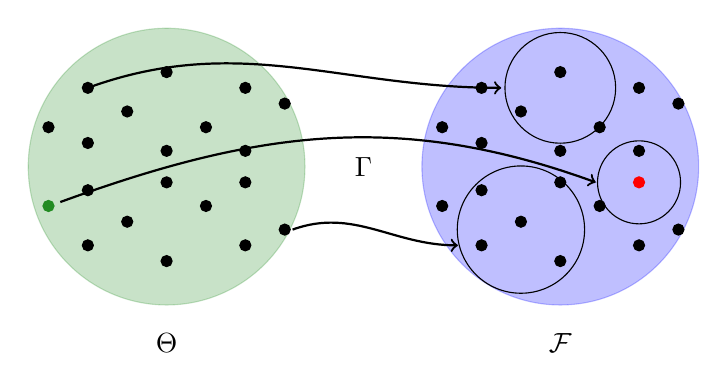
\begin{tikzpicture}
		\filldraw[blue, nearly transparent] (5,0) circle(50pt);
		\filldraw[ForestGreen, nearly transparent] (0,0) circle(50pt);
		\node[below] at (5,-2) {$\mathcal{F}$};
		\node[below] at (0,-2) {$\Theta$};
		\node at (2.5,0) {$\Gamma$};
		\filldraw (5,1.2) circle(2pt);
		\filldraw (5,.2) circle(2pt);
		\filldraw (3.5,0.5) circle(2pt);
		\filldraw (4,0.3) circle(2pt);
		\filldraw (4.5,0.7) circle(2pt);
		\filldraw (5.5,0.5) circle(2pt);
		\filldraw (6,0.2) circle(2pt);
		\filldraw (6.5,0.8) circle(2pt);
		\filldraw (4,1) circle(2pt);
		\filldraw (6,1) circle(2pt);
		\filldraw (5,-1.2) circle(2pt);
		\filldraw (5,-.2) circle(2pt);
		\filldraw (3.5,-0.5) circle(2pt);
		\filldraw (4,-0.3) circle(2pt);
		\filldraw (4.5,-0.7) circle(2pt);
		\filldraw (5.5,-0.5) circle(2pt);
		\filldraw[red] (6,-0.2) circle(2pt);
		\filldraw (6.5,-0.8) circle(2pt);
		\filldraw (4,-1) circle(2pt);
		\filldraw (6,-1) circle(2pt);
		
		\filldraw (0,1.2) circle(2pt);
		\filldraw (0,.2) circle(2pt);
		\filldraw (-1.5,0.5) circle(2pt);
		\filldraw (-1,0.3) circle(2pt);
		\filldraw (-.5,0.7) circle(2pt);
		\filldraw (.5,0.5) circle(2pt);
		\filldraw (1,0.2) circle(2pt);
		\filldraw (1.5,0.8) circle(2pt);
		\filldraw (-1,1) circle(2pt);
		\filldraw (1,1) circle(2pt);
		\filldraw (0,-1.2) circle(2pt);
		\filldraw (0,-.2) circle(2pt);
		\filldraw[ForestGreen] (-1.5,-0.5) circle(2pt);
		\filldraw (-1,-0.3) circle(2pt);
		\filldraw (-.5,-0.7) circle(2pt);
		\filldraw (.5,-0.5) circle(2pt);
		\filldraw (1,-0.2) circle(2pt);
		\filldraw (1.5,-0.8) circle(2pt);
		\filldraw (-1,-1) circle(2pt);
		\filldraw (1,-1) circle(2pt);
		
		\draw[->,thick] (-1.35,-0.45) to[out=20,in=160] (5.45,-0.2);
		\draw (6,-0.2) circle(15pt);
		\draw[->,thick] (-1,1) to[out=20,in=180] (4.25,1);
		\draw (5,1) circle(20pt);
		\draw[->,thick] (1.6,-0.8) to[out=20,in=180] (3.7,-1);
		\draw (4.5,-0.8) circle(23pt);
	\end{tikzpicture}
\end{figure}

\begin{remark}
	If likelihood is specified, $\Gamma(\cdot)$ is a singleton. In GMM, we have that $\Gamma(\theta) = \{F(W) \in \mathcal{F}: \expect_F g(W;\theta) = 0\}$, so $\theta_0$ is identified if $F \in \Gamma(\theta_0)$ implies that $\Gamma^{-1}(F) = \{\theta_0\}$. We usually consider $\theta$ identified if the above holds for all possible true values.
\end{remark}

\begin{remark}
	This can be used to motivate some extensions, not pursued here:
	\begin{enumerate}
		\item \blue{Partial Identification}: $\Gamma^{-1}(F_0)$ is a set. This is completely uninformative if it is $\Theta$, and point-identifying if it is $\{\theta_0\}$. Often it is somewhere in between.
		\item \blue{Irregular Identification} or \blue{Ill-posed Inverse Problems}: $\Gamma^{-1}(\cdot)$ is sufficiently ill-behaved so that identifiability formally obtains but, for example, convergence of the empirical distribution $F_n$ to $F$ may imply convergence of $\Gamma^{-1}(F_n)$ to $\Gamma^{-1}(F)$ at a slower, if any, rate.
	\end{enumerate}
\end{remark}
\begin{remark}
	In many cases, the distribution of regressors $X$ is not informative about $\theta$. That is, we can write \[f(Y,X;\theta) = f_y(Y\mid X;\theta) f_X(X)\]then we have simplification 
	\begin{align*}
		\hat{\theta}_{ML} &= \argmax_{\theta\in\Theta} \sum_{i=1}^n \log f(Y,X;\theta) \\ &= \argmax_{\theta\in\Theta} \sum_{i=1}^n \parl \log f_y(Y\mid X;\theta) + \log f_X(X)\parr \\
		&= \argmax_{\theta\in\Theta} \sum_{i=1}^n \log f_y(Y \mid X;\theta)
	\end{align*}
	In practice, many ML estimators reflect this simplification. For the purpose of theoretical analysis, we always write the estimator as maximizing the complete likelihood.
\end{remark}

Consistency of maximum likelihood follows from the $m$-estimator consistency result above. In fact:

\begin{theorem}
	$\theta_0$ uniquely maximizes $\expect \log f(W;\theta)$ if and only if $\theta \ne \theta_0$ implies that $\prob\{f(W;\theta) \ne f(W;\theta_0)\} > 0$.
\end{theorem}
\begin{proof}
	We write
	\begin{align*}
		\expect \log f(W;\theta) - \expect \log f(W;\theta_0) &= \expect \log \frac{f(W;\theta)}{f(W;\theta_0} \le \log \expect \frac{f(W;\theta)}{f(W;\theta_0} \\
		= \log \int \frac{f(w;\theta)}{f(w;\theta_0)} f(w;\theta_0)dw &= \log \int f(w;\theta) dw = \log 1 = 0
	\end{align*}
	where the inequality is Jensen's Inequality, and it is strict unless \[\frac{f(W;\theta)}{f(W;\theta_0)} \text{ constant almost surely } \Longleftrightarrow \prob\{f(W;\theta) \ne f(W;\theta_0)\} = 0\]
\end{proof}

\begin{remark}
	The structure of maximum likelihood allows us to both verify the ``CLT assumption'' and provide an expression for the asymptotic variance:
	\begin{align*}
		\int f(w;\theta)dw &= 1 \forall \theta \in \Theta \\
		\Longrightarrow \int \frac{\partial f(w;\theta_0)}{\partial \theta}dw &= 0 \\
		\Longrightarrow \int  \frac{\partial \log f(w;\theta_0)}{\partial \theta} f(w;\theta_0)dw &= 0 \\
		\Longrightarrow \expect \parl \frac{\partial \log f(w;\theta_0)}{\partial \theta}\parr &= 0
	\end{align*}
	This result, called the \blue{score equation}, is important in its own right: it tells us that maximum likelihood can be interpreted as a method of moments estimator. Taking derivatives again, we get:
	\begin{align*}
		\int \frac{\partial^2 \log f(w;\theta_0)}{\partial \theta \partial \theta'}f(w;\theta_0)dw + \int \frac{\partial \log f(w;\theta_0)}{\partial \theta}\frac{\partial \log f(w;\theta_0)}{\partial \theta'} f(w;\theta_0) dw &= 0 \\
		\Longrightarrow \expect \parl \frac{\partial^2 \log f(w;\theta_0)}{\partial \theta \partial \theta'}\parr + \expect \parl \frac{\partial \log f(w;\theta_0)}{\partial \theta}\frac{\partial \log f(w;\theta_0)}{\partial \theta'}\parr &= 0 \\
		\Longrightarrow  \expect \parl \frac{\partial^2 \log f(w;\theta_0)}{\partial \theta \partial \theta'}\parr &= - \expect \parl \frac{\partial \log f(w;\theta_0)}{\partial \theta}\frac{\partial \log f(w;\theta_0)}{\partial \theta'}\parr
	\end{align*}
	The last line is, of course, the \blue{information matrix equality}! Now we write
	\[Q_n(\theta_0) = \frac{1}{n} \sum_{i=1}^n \log f(w_i;\theta_0) \Longrightarrow \frac{\partial Q_n(\theta_0)}{\partial \theta} = \frac{1}{n} \sum_{i=1}^n \frac{\partial \log f(w_i;\theta_0)}{\partial \theta}\]But we just showed that $\expect \parl \frac{\partial \log f(w;\theta_0)}{\partial \theta}\parr = 0$. We thus have from the CLT:
	\[
	\sqrt{n} \frac{\partial Q_n(\theta_0)}{\partial \theta} \todist \normal \parl 0, \expect \parl \frac{\partial \log f(w;\theta_0)}{\partial \theta}\frac{\partial \log f(w;\theta_0)}{\partial \theta'}\parr\parr
	\]
	This establishes part (4) of Assumptions~\ref{ass:asymptotics_extremum}. Substituting these findings into the theorem, we get 
	\begin{align*}
		\sqrt{n}(\hat{\theta} - \theta_0) &\todist \normal \Bigg( 0,\Bigg(\underbrace{ \expect \parl \frac{\partial^2 \log f(w;\theta_0)}{\partial \theta \partial \theta'}\parr}_{\mathcal{H}}\Bigg)^{-1} \underbrace{\expect \parl \frac{\partial \log f(w;\theta_0)}{\partial \theta}\frac{\partial \log f(w;\theta_0)}{\partial \theta'}\parr}_{S = -\mathcal{H}} \Big( \underbrace{\expect(\cdot)}_{\mathcal{H}}\Big)^{-1}\Bigg)\\
		&= \normal\parl0,-\mathcal{H}^{-1}\parr
	\end{align*}
	where we use the Information Matrix Equality. Under our i.i.d. assumption, $\mathcal{H}$ is the \blue{(Fisher) information matrix} $\mathbb{I}(\theta_0)$, so ML asymptotically attains the \blue{Cramer-Rao lower bound}. In fact, it is known (we will not show it) that ML is asymptotically efficient in the sense that it has the smallest asymptotic variance in a large class of regular estimators. This creates a strong case for using ML, as long as you are willing to specify a likelihood and can compute the ML estimator.
\end{remark}


\begin{remark}
	Whenever we have a complete likelihood, we can use maximum likelihood, but we could also use GMM -- knowledge of the likelihood implies knowledge of the moment conditions, definitely the score equations but possibly others. So could GMM match (or possibly beat) the performance of ML? No! we have directly that 
	\begin{align*}
		(G'S^{-1}G)^{-1} &- \mathbb{I}(\theta_0)^{-1} \text{ is positive semi-definite} \\
		(G'S^{-1}G)^{-1} &= \mathbb{I}(\theta_0)^{-1} \text{ if } g(w,\theta) = \frac{\partial \log f(w;\theta_0)}{\partial \theta}
	\end{align*}
	Thus, GMM cannot asymptotically beat ML estimation, as $\avar(\hat{\theta}_{GMM}) \ge \avar(\hat{\theta}_{ML})$. If the likelihood is known, GMM can trivially match ML by mimicking it, but since those moment conditions would reflect likelihood information, we cannot in general get ML efficiency without knowing the likelihood.
\end{remark}

\begin{example}
	Suppose we want to test $\hyp_0: r(\theta) = 0$ where $r(\cdot)$ is a known function whose Jacobian $R(\cdot)$ is both continuous and has full rank at $\theta_0$. The \blue{trinity} of test statistics are:
	\begin{enumerate}
		\item \blue{Wald}: $W = nr(\hat{\theta})'(R(\hat{\theta})\hat{\Sigma}^{-1}R(\hat{\theta})')^{-1}r(\hat{\theta})$
		\item \blue{Likelihood Ratio}: $LR = 2n(Q_n(\hat{\theta})- Q_n(\tilde{\theta}))$
		\item \blue{Lagrange Multiplier}: $LM = n \frac{\partial Q_n(\tilde{\theta})'}{\partial \theta} \tilde{\Sigma}^{-1} \frac{\partial Q_n(\tilde{\theta})}{\partial \theta}$
	\end{enumerate}
	where $\tilde{\theta}$ is the \blue{constrained estimator} \[\tilde{\theta} \equiv \argmin_{\theta\in\Theta} Q_n(\theta) \st r(\theta) = 0\]and where $(\hat{\Sigma},\tilde{\Sigma})$ estimate the outer product of gradients at $(\hat{\theta},\tilde{\theta})$. We can illustrate the hypotheses as:
	\begin{figure}[H]
		\centering
		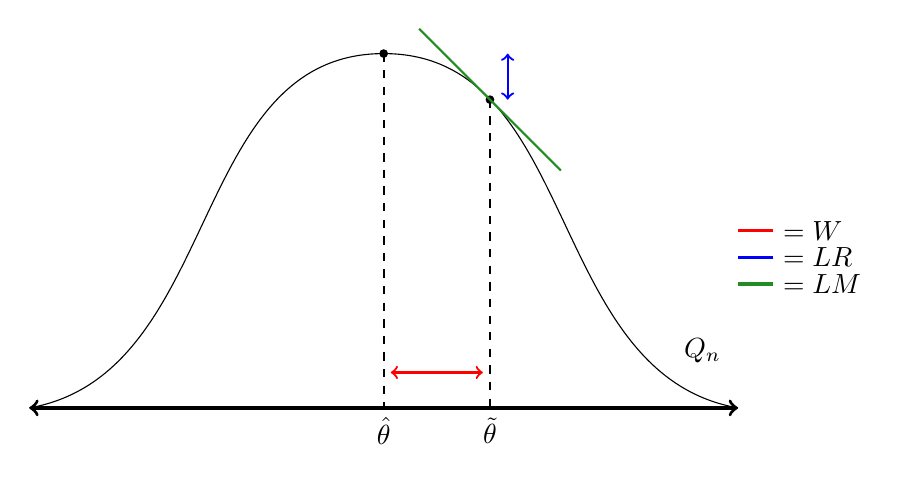
\begin{tikzpicture}[scale=0.45]
			\draw[<->,very thick] (-10,0)--(10,0);
			\draw (-10,0) to[out=10,in=180] (0,10) to[out=0,in=170] (10,0);
			\filldraw (0,10) circle(3pt);
			\draw[dashed, thick] (0,10)--(0,0);
			\node[below] at (0,0) {$\hat{\theta}$};
			\node[above] at (9,1) {$Q_n$};
			\filldraw (3,8.7) circle(3pt);
			\draw[dashed, thick] (3,8.7)--(3,0);
			\node[below] at (3,0) {$\tilde{\theta}$};
			\draw[thick,<->,red] (0.2,1)--(2.8,1);
			\draw[thick, <->,blue] (3.5,8.7)--(3.5,10);
			\draw[thick, ForestGreen] (5,6.7)--(3,8.7)--(1,10.7);
			
			\node[right] at (11,5) {$=W$};
			\node[right] at (11,4.25) {$=LR$};
			\node[right] at (11,3.5) {$=LM$};
			\draw[very thick, red] (11,5)--(10,5);
			\draw[very thick, blue] (11,4.25)--(10,4.25);
			\draw[very thick, ForestGreen] (11,3.5)--(10,3.5);
		\end{tikzpicture}
	\end{figure}
\end{example}

\begin{assumption}\label{ass:test_equiv}
	We assume that:
	\begin{enumerate}
		\item $\sqrt{n}(\hat{\theta} - \theta_0) = -\mathcal{H}^{-1}\sqrt{n} \frac{\partial Q_n(\theta_0)}{\partial \theta} + o_P(1)$
		\item $\frac{\partial Q_n(\theta_0)}{\partial \theta} \todist \normal(0,\Sigma)$, with $\Sigma$ positive definite
		\item $\sqrt{n}(\tilde{\theta} - \theta_0) = O_P(1)$
		\item $\Sigma = -\mathcal{H}$
	\end{enumerate}
\end{assumption}


\begin{theorem}
	Under Assumptions~\ref{ass:test_equiv}, all of the tests (Wald, Likelihood Ratio, and Lagrange Multiplier) converge in distribution to $\chi^2_{\#r}$. Furthermore, they are asymptotically equivalent.
\end{theorem}
\begin{remark}
	We will take on faith that $\sqrt{n}(\tilde{\theta} - \theta_0) = O_P(1)$, Hayashi shows it from the theory of constrained estimators. We will only spell out the details for maximum likelihood, for everything else $\mathcal{H}$ must be redefined. We do need that $\mathcal{H} = -\Sigma$, meaning that ML is well-specified. We will come back to misspecified models.
\end{remark}
\begin{proof}
	(Only of the convergence statement). The argument for the Wald statistic is entirely above. The first order condition for the constrained estimation problem can be written as\[\sqrt{n}\frac{\partial Q_n(\tilde{\theta})}{\partial \theta} + \sqrt{n}R(\tilde{\theta})'\gamma_n = 0 \qquad ; \qquad \sqrt{n}r(\tilde{\theta}) = 0\] We can use the Mean Value Theorem to write 
	\begin{align*}
		r(\tilde{\theta}) &= r(\theta_0) + R(\bar{\theta})(\tilde{\theta}-\theta_0) \\
		\Longrightarrow \sqrt{n}r(\tilde{\theta}) &= \sqrt{n}R(\bar{\theta})(\tilde{\theta}-\theta_0) \\
		&= \underbrace{\sqrt{n}(R(\bar{\theta}) - R(\theta_0))(\tilde{\theta}-\theta_0)}_{\toprob 0} + \sqrt{n}R(\theta_0)(\tilde{\theta}-\theta_0) \\
		&= R(\theta_0) \cdot \sqrt{n} (\tilde{\theta} - \theta_0) + o_P(1)
	\end{align*}
	Next, a Taylor expansion of $\frac{\partial Q_n(\theta)}{\partial \theta}$about $\theta_0$ yields 
	\[
	\sqrt{n} \frac{\partial Q_n(\tilde{\theta})}{\partial \theta} = \underbrace{\sqrt{n} \frac{\partial Q_n(\theta_0)}{\partial \theta}}_{\todist \normal(0,\Sigma)} + \sqrt{n}\underbrace{\frac{\partial^2 Q_n(\theta_0)}{\partial \theta\partial \theta'}}_{\toprob \mathcal{H}}(\tilde{\theta} - \theta_0)+o_P(1)
	\]
	The second and third assumptions now imply that $\sqrt{n} \frac{\partial Q_n(\tilde{\theta})}{\partial \theta}$, and thus $\sqrt{n}\gamma_n$, are of order $O_P(1)$. This in turn allows us to write
	\[
	R(\tilde{\theta})' \sqrt{n} \gamma_n = R(\theta_0)'\sqrt{n}\gamma_n + (R(\tilde{\theta}) - R(\theta_0))' \sqrt{n}\gamma_n =  R(\theta_0)'\sqrt{n}\gamma_n + o_P(1)
	\] 
	Next, collecting of terms. We have:
	\begin{align*}
		\sqrt{n}r(\tilde{\theta}) &= 0 \\
		\sqrt{n}r(\tilde{\theta})  &= R(\theta_0) \cdot \sqrt{n} (\tilde{\theta} - \theta_0) + o_P(1) \\
		\Longrightarrow R(\theta_0) \cdot \sqrt{n} (\tilde{\theta} - \theta_0) &= o_P(1)
	\end{align*}
	as well as:
	\begin{align*}
		\sqrt{n}\frac{\partial Q_n(\tilde{\theta})}{\partial \theta} &+ \sqrt{n}R(\tilde{\theta})'\gamma_n = 0 \\
		\sqrt{n}\frac{\partial Q_n(\tilde{\theta})}{\partial \theta} &= \sqrt{n} \frac{\partial Q_n(\theta_0)}{\partial \theta} + \mathcal{H}\sqrt{n}(\tilde{\theta}-\theta_0) + o_P(1) \\
		R(\tilde{\theta})' \sqrt{n}\gamma_n &= R(\theta_0)' \sqrt{n}\gamma_n + o_P(1)\\
		\Longrightarrow \mathcal{H} \sqrt{n} (\tilde{\theta}-\theta_0) +  R(\theta_0)' \sqrt{n}\gamma_n  &= -\sqrt{n}\frac{\partial Q_n(\theta_0)}{\partial \theta} + o_P(1)
	\end{align*}
	This implicitly characterizes the joint distribution, but we can make it explicit, by consolidating into 
	\[
	\matrixc{\mathcal{H} & R' \\ R & 0} \cdot \matrixc{\sqrt{n}(\tilde{\theta}-\theta_0) \\ \sqrt{n}\gamma_n} = \matrixc{ -\sqrt{n}\frac{\partial Q_n(\theta_0)}{\partial \theta} \\ 0} + o_P(1)
	\]
	which implies that
	\[
	\sqrt{n} \matrixc{\tilde{\theta} - \theta_0 \\ \gamma_n} = \matrixc{-\mathcal{H}^{-1} + \mathcal{H}^{-1}R'(R\mathcal{H}^{-1}R')^{-1}R\mathcal{H}^{-1} \\- (R\mathcal{H}^{-1}R')^{-1}R\mathcal{H}^{-1}}\sqrt{n} \frac{\partial Q_n(\theta_0)}{\partial \theta} + o_P(1)
	\]
	This gets us the LM statistic fairly quickly:
	\begin{align*}
		\sqrt{n} \gamma_n &= - (R\mathcal{H}^{-1}R')^{-1}R\mathcal{H}^{-1}\sqrt{n} \frac{\partial Q_n(\theta_0)}{\partial \theta} + o_P(1) \\
		&\todist \normal \parl 0, (R\mathcal{H}^{-1}R')^{-1}R\mathcal{H}^{-1}\Sigma \mathcal{H}^{-1}R'(R\mathcal{H}^{-1}R')^{-1}\parr \\
		&= \normal\parl 0, (R\Sigma^{-1}R')^{-1}\parr \\
		&\Longrightarrow \sqrt{n}\gamma_n' R\Sigma^{-1}R' \sqrt{n}\gamma_n \todist \chi^2_{\#r}
	\end{align*}
	We conclude with another MVT expansion:
	\[
	Q_n(\tilde{\theta}) = Q_n(\hat{\theta}) + \frac{\partial Q_n(\hat{\theta})}{\partial \theta} (\tilde{\theta} - \hat{\theta}) + \frac{1}{2}  (\tilde{\theta} - \hat{\theta}) ' \frac{\partial^2 Q_n(\bar{\theta}}{\partial \theta \partial \theta'}  (\tilde{\theta} - \hat{\theta}) 
	\]
	However, the first partial of $Q_n(\cdot)$ is zero (almost surely) and the second partial converges to the (negative) curvature. Thus,
	\begin{align*}
		2n(Q_n(\hat{\theta}) - Q_n(\tilde{\theta})) &= -\sqrt{n}(\tilde{\theta} - \hat{\theta})  (\mathcal{H} + o_P(1)) \sqrt{n} (\tilde{\theta} - \hat{\theta}) \\ &= -\sqrt{n}(\tilde{\theta} - \hat{\theta})  \mathcal{H}\sqrt{n} (\tilde{\theta} - \hat{\theta}) + o_P(1)
	\end{align*}
	We can substitute from the matrix equation to get 
	\begin{align*}
		\sqrt{n} (\tilde{\theta} - \hat{\theta}) &= -(\mathcal{H}^{-1} - \mathcal{H}^{-1}R'(R\mathcal{H}^{-1}R')^{-1}R\mathcal{H}^{-1})\sqrt{n} \frac{\partial Q_n(\theta_0)}{\partial \theta} + \mathcal{H}^{-1}\sqrt{n}\frac{\partial Q_n(\theta_0)}{\partial \theta} + o_P(1) \\
		&= \mathcal{H}^{-1}R'(R\mathcal{H}^{-1}R')^{-1}R\mathcal{H}^{-1}\sqrt{n} \frac{\partial Q_n(\theta_0)}{\partial \theta} + o_P(1)
	\end{align*}
	This determines the distribution of the LR statistic. The rest is algebra:
	\begin{align*}
		2n(Q_n(\hat{\theta}) - Q_n(\tilde{\theta})) &\approx - \sqrt{n} \frac{\partial Q_n(\theta_0)}{\partial \theta}\parl \mathcal{H}^{-1}R'(R\mathcal{H}^{-1}R')^{-1}R\mathcal{H}^{-1}\parr' \mathcal{H} \mathcal{H}^{-1}R'(R\mathcal{H}^{-1}R')^{-1}R\mathcal{H}^{-1} \sqrt{n} \frac{\partial Q_n(\theta_0)}{\partial \theta} \\
		&= - \sqrt{n} \frac{\partial Q_n(\theta_0)}{\partial \theta}  \mathcal{H}^{-1}R'(R\mathcal{H}^{-1}R')^{-1}R\mathcal{H}^{-1} \sqrt{n} \frac{\partial Q_n(\theta_0)}{\partial \theta} \\
		&= \sqrt{n} \frac{\partial Q_n(\theta_0)}{\partial \theta}  \Sigma^{-1}R'(R\Sigma^{-1}R')^{-1}R\Sigma^{-1} \sqrt{n} \frac{\partial Q_n(\theta_0)}{\partial \theta} 
	\end{align*}
	Recalling that $ \sqrt{n} \frac{\partial Q_n(\theta_0)}{\partial \theta} \todist \normal(0,\Sigma)$, we have 
	\begin{align*}
		R\Sigma^{-1} \sqrt{n} \frac{\partial Q_n(\theta_0)}{\partial \theta}  &\todist \normal\parl 0, R\Sigma^{-1} \Sigma \Sigma^{-1} R'\parr = \normal(0,R\Sigma^{-1}R') \\
		\Longrightarrow LR &\todist \chi^2_{\#r}
	\end{align*}
\end{proof}

\begin{remark}
	Why is it called the likelihood ratio statistic? If we take the likelihood literally, then
	\[
	n (Q_n(\hat{\theta}) - Q_n(\tilde{\theta})) = \sum_{i=1}^n \ell(\hat{\theta}) - \sum_{i=1}^n \ell(\tilde{\theta})  = \frac{f(W_1,\dots,W_n;\hat{\theta})}{f(W_1,\dots,W_n;\tilde{\theta})}
	\]
	The additional factor of 2 aligns the statistic with the others, but the interpretation of $Q_n(\cdot)$ is not essential.
\end{remark}

\section{Worked Examples}

\begin{example}\red{Poisson}
	Let $Y$ be distributed i.i.d. Poisson with true parameter $\lambda_0 > 0$. Recall that $\prob\{Y = k\} = \lambda^k e^{-\lambda} / k!$, with mean and variance $\lambda$. Intuitively, we of course will estimate $\lambda$ using $\bar{y}$, and the Lindeberg-L\'{e}vy CLT (see Econometrics I notes for a full treatment) immediately yields $\sqrt{n}(\bar{y}-\lambda_0 ) \todist \normal(0,\lambda_0)$. To analyze this as an example of maximum likelihood, we write:
	\begin{align*}
		Q_n(\lambda) &= \frac{1}{n} \sum_i \parl y_i \log \lambda - \lambda - \log(y_i!)\parr \\
		\frac{\partial Q_n(\lambda)}{\partial \lambda} &= \frac{1}{n}\sum_i \parl \frac{y_i}{\lambda}-1\parr \\
		\frac{\partial^2 Q_n(\lambda)}{\partial \lambda^2} &= -\frac{1}{n}\sum_i \frac{y_i}{\lambda^2} \\
		Q(\lambda) &= \expect\barl Y \log \lambda - \lambda - \log Y!\barr  \\
		\frac{\partial Q(\lambda)}{\partial \lambda} &= \expect \barl \frac{Y}{\lambda} - 1\barr \\
		\frac{\partial^2Q(\lambda)}{\partial \lambda^2} &= - \expect \barl \frac{Y}{\lambda^2}\barr
	\end{align*}
	We can see that we have strict concavity, so the maximum likelihood estimator is characterized by the first order condition. In particular, 
	\[
	\frac{1}{n}\sum_i \parl \frac{y_i}{\lambda} - 1\parr = 0 \Longrightarrow \hat{\lambda}_{ML} = \bar{y}
	\]
	We can next apply the consistency theorem for extremum estimators. Pointwise convergence of $Q_n$ to $Q$ is clear. The parameter space is not compact but since $Q_n$ is strictly concave and $\lambda$ is a scalar, that is not necessary. Of the conditions for asymptotic normality, the first was established above, the second holds as long as $\lambda > 0$, the third is obvious, the fourth holds because $Y$ is i.i.d. with first and second moments $\lambda_0$, meaning that \[\sqrt{n}\frac{\partial Q_n(\lambda_0)}{\partial \lambda} = \sqrt{n}\frac{1}{n} \sum_i \parl \frac{Y_i}{\lambda_0}- 1\parr \todist \normal(0,\lambda_0^{-1})\]The fifth condition follows directly, the sixth we have directly because $\frac{\partial^2 Q(\lambda_0)}{\partial \lambda^2} = -\frac{1}{\lambda_0}$, and the last because $\lambda_0 > 0$. Thus, the consistency theorem applies, and we have that\[\sqrt{n}(\hat{\lambda}-\lambda_0) \todist \normal(0,(-\lambda_0^{-1})^{-1}\lambda_0^{-1} (-\lambda_0^{-1})^{-1}) = \normal(0,\lambda_0)\]Note that these results do not apply if $\lambda_0 = 0$, because interiority is violated. In this case, we have an actual failure of result -- the distribution of both $Y$ and $\bar{y}$ will be degenerate at 0. The above result does not uniformly hold as $\lambda_0 \to 0$; it fails along drifting parameters of the form $\lambda_n = \gamma / \sqrt{n}$. 
\end{example}

\begin{example}
	\red{Binary Response} Binary response models can generally be expressed in the form \[ Y = \ones\{\phi(X,\varepsilon;\theta_0) \ge 0\}\]which is frequently specialized to \[Y = \ones\{X'\beta-\varepsilon \ge 0\} \iff \prob\{Y = 1 \mid X\} = \prob\{\varepsilon \le X'\beta\} = F_\varepsilon(X'\beta)\]Assume that $\expect XX'$ is nonsingular and that $F_\varepsilon$ is strictly increasing. Then the model is identified up to scale normalization and (if $X$ has a constant) a location normalization. Other than that, different assumptions about $F_\varepsilon$ lead to different models. If we assume that $\varepsilon$ is logistically distributed, we have the logit model \[\prob\{Y = 1 \mid X\} = \frac{\exp(X'\beta)}{1+\exp(X'\beta)}\]Which admits log likelihood \[\log f(Y \mid X ; \theta) = Y \log \frac{\exp(X'\beta)}{1 + \exp(X'\beta)} + (1-Y) \log \frac{1}{1+\exp(X'\beta)}\]and the maximum likelihood estimator is characterized as a maximizer of \begin{align*} Q_n(\beta) &= \frac{1}{n} \sum_i \parl Y_i \log \frac{\exp(X'\beta)}{1 + \exp(X'\beta)} + (1-Y) \log \frac{1}{1+\exp(X'\beta)}\parr \\ &= \frac{1}{n} \sum_i \parl Y_iX_i'\beta - Y_i \log(1 + \exp(X_i'\beta)) - (1-Y_i)\log(1 + \exp(X'_i\beta))\parr \\ &= \frac{1}{n} \sum_i  \parl Y_iX_i'\beta - \log(1 + \exp(X_i'\beta))\parr \end{align*}We can thus write\begin{align*} \frac{\partial Q_n(\beta)}{\partial \beta} &= \frac{1}{n}\sum_i \parl Y_iX_i - \frac{\exp(X_i'\beta)}{1 + \exp(X_i'\beta)}X_i\parr = \frac{1}{n}\sum_i \parl Y_i - F_\varepsilon(X_i'\beta)\parr X_i \\ \frac{\partial^2Q_n(\beta)}{\partial \beta \partial \beta'} &= -\frac{1}{n} \sum_i F_\varepsilon(X_i'\beta)(1 - F_\varepsilon(X_i'\beta))X_iX_i'\end{align*}where we apply the formula $F(t) = e^t / (1+e^t) \Longrightarrow F'(t) = F(t)(1-F(t))$ to the CDF. As in the first example, we could directly attain consistency and asymptotic normality by checking the conditions, which all hold. 
	
	\begin{remark}
		If we replaced sample averages wtih expectations in the above, we would have \begin{align*} \frac{\partial Q(\beta)}{\partial \beta} &= \expect\parl (Y - F_\varepsilon(X'\beta)) X\parr \\ \frac{\partial^2 Q(\beta)}{\partial \beta \partial \beta'} &= -\expect \parl F_\varepsilon(X'\beta)(1-F_\varepsilon(X'\beta))XX'\parr \end{align*}At first glance, the information matrix equality may not appear obvious. However, we can convert this to: \begin{align*} &\quad\;\hspace{.02cm} \expect\barl  \parl (Y - F_\varepsilon(X'\beta)) X\parr\parl (Y - F_\varepsilon(X'\beta)) X\parr'\barr \\ &= \expect \barl \parl Y-F_\varepsilon(X'\beta) \parr^2 XX'\barr \\ &= \expect \barl \expect \barl (Y - F_\varepsilon(X_i'\beta))^2 \mid X\barr XX'\barr \\ &= \expect\barl \var(Y\mid X) XX'\barr \\ &= \expect \barl F_\varepsilon(X'\beta)(1-F_\varepsilon(X'\beta))XX'\barr \\ &= - \frac{\partial^2Q(\beta)}{\partial \beta \partial \beta'}\end{align*}where we use the Law of Iterated Expectations and the knowledge that $Y$ is distributed Bernoulli once we condition on $X$.
	\end{remark}
	\begin{remark}
		We could also estimate this model using GMM. To do so, we need a function $g$ of the dimensionality of $X$ such that $\expect g(Y,X;\beta) = 0$. As a general rule, if conditional expectations can be written out, they immediately give rise to such functions. In the current example, from LIE we get \[\expect(X(Y - F_\varepsilon(X'\beta))) = \expect(X\expect(Y -F_\varepsilon(X'\beta)\mid X)) = 0\]so our GMM estimator is defined by the sample analog \[\frac{1}{n}\sum_i X_i(Y_i - F_\varepsilon(X'_i\hat{\beta})) = 0\]So the estimators algebraically coincide! The natural GMM estimator uses the score equations as moment conditions and therefore is exactly the ML estimator -- replicating even the variance precisely.
	\end{remark}
	
	\begin{remark}
		If we consider $\expect\barl Y |X\barr = G(X'\beta)$, we consider $G(\cdot)$ the \blue{link function} and $X'\beta$ the \blue{linear index}. If we shift this by a sigmoid, we can convert this to logit or probit models quite easily. For the probit, we have that\[\expect \barl Y \mid X \barr = \Phi(X'\beta) \iff Y = \ones\{X'\beta - \varepsilon \ge 0\},\varepsilon \sim \normal(0,1)\]In logit and probit models, coefficients are in general sign interpretable; relative absolute values are \emph{sometimes} interpretable; absolute values without context are not interpretable. We have that \[\frac{\partial \expect(Y \mid X)}{\partial X_j} = \beta_j \cdot g(X'\beta)\]where $g(\cdot) \equiv G'(\cdot)$. The sign of this term will be the sign of the coefficient, as $g(\cdot)$ is positive always, but the marginal effect depends on the magnitude of $g(\cdot)$ which is not in general known. Put plainly, the marginal effect of $X_j$ on $Y$ is now described by two numbers, and depends on where $X_j$ is. If you \emph{need} an interpretable number, there are some options: marginal effect at a particular fixed $X$, average estimated effect which is $\expect_n \hat{\beta}_j\cdot g(X'\hat{\beta})$, and the estimated effect at the average which is $\hat{\beta}_j \cdot g(\expect_n X'\hat{\beta})$. 
	\end{remark}
\end{example}

\begin{example}
	\red{Type II Tobit} The following model is known as \blue{Type II Tobit}: \begin{align*} Y_1\opt &= X_1'\beta_1 + \varepsilon_1 \\ Y_2\opt &= X_2'\beta_2 + \varepsilon_2 \\ Y_1 &= \ones\{Y_1\opt \ge 0\} \\ Y_2 &= Y_2\opt \cdot \ones\{Y_1\opt \ge 0\} \\ \matrixp{\varepsilon_1 \\ \varepsilon_2} &\sim \normal\parl 0, \matrixp{\sigma_1^2 & \rho\sigma_1\sigma_2 \\ \rho \sigma_1 \sigma_2 & \sigma_2^2}\parr\end{align*}
	Note that you observe only $Y_1$ and $Y_2$, not the respective latent starred variables. The motivation here is that the  equation of interest is for $Y_2\opt$, called the \blue{outcome equation}. The equation for $Y_1\opt$ is called the \blue{selection equation}. The parameter of interest is $\beta_2$. If we observed $Y_2\opt$, we could estimate it by straight OLS. However, since we are selecting for when $Y_1\opt \ge 0$, we are selecting for high values of $\varepsilon_1$. As long as $\rho \ne 0$, the correlation between $\varepsilon_1$ and $\varepsilon_2$ means that we have selection also in the sample of interest.
	
	The motivating examples here are typically that the decision to enter some market is dependent on a threshold that does not affect the values in the market -- think if the decision to enter the labor force is dependent on having children, but wages are not directly determined by children, or if foreign aid is dependent on a certain political stance but the level of foreign aid does not depend on said political stance.
	
	The selection model in the first and third equations gives us the likelihood\[\prob\{Y_1 = 0 \mid X_1,X_2;\theta\} = \Phi\parl - \frac{X_1'\beta_1}{\sigma_1}\parr\]Thus, the likelihood of $Y_2$ conditional on $X_1,X_2$, and $Y_1 = 1$ (meaning $Y_2$ is observed at all) is:
	\begin{align*}
		f(Y_2 \mid X_1,X_2,Y_1=1;\theta) &= \prob\{Y_1 = 1\mid X_1,X_2;\theta) \cdot f(Y_2 \mid X_1,X_2 ; \theta) / \Phi\parl \frac{X_1'\beta_1}{\sigma_1}\parr \\&= \frac{1}{\sigma_2} \Phi \parl \frac{X_1'\beta_1 + \rho \frac{\sigma_1}{\sigma_2} (Y_2 - X_2'\beta_2)}{\sigma_1 \sqrt{1-\rho^2}}\parr \phi \parl \frac{Y_2 - X_2'\beta}{\sigma_2}\parr / \Phi \parl \frac{X_1'\beta_1}{\sigma_1}\parr
	\end{align*}
	where we used the (conditional) distributions of the errors.
	
	We will establish identification using the thought experiment: If we had perfect knowledge of the above likelihoods, could we back out the true parameter values? Actually, the answer is no. The probit part of the model identifies the ratio $\beta_1 / \sigma_1$, but neither parameter on their own. The natural way to get identification is to normalize $\sigma_1 = 1$, and work to identify all other parameters. This gives us the simplification:
	\begin{align*}
		\prob\{Y_1 = 0 \mid X_1,X_2;\theta\} &= \Phi (-X_1'\beta_1) \\f(Y_2 \mid X_1,X_2,Y_1=1;\theta) &=\frac{1}{\sigma_2} \Phi \parl \frac{X_1'\beta_1 +  \frac{\rho}{\sigma_2} (Y_2 - X_2'\beta_2)}{ \sqrt{1-\rho^2}}\parr \phi \parl \frac{Y_2 - X_2'\beta}{\sigma_2}\parr / \Phi \parl X_1'\beta_1\parr
	\end{align*}
	With $\sigma_1 = 1$, our selection equation now identifies $\beta_1$, so we will treat $\Phi(X_1'\beta_1)$ as known. Define:
	\begin{align*}
		\tilde{f}(Y_2 \mid X_1,X_2;\theta) &= \frac{1}{\sigma_2} \Phi \parl \frac{X_1'\beta_1 +  \frac{\rho}{\sigma_2} (Y_2 - X_2'\beta_2)}{ \sqrt{1-\rho^2}}\parr \phi \parl \frac{Y_2 - X_2'\beta}{\sigma_2}\parr 
	\end{align*}
	The partials are:
	\begin{align*}
		\frac{\partial \tilde{f}(\cdot)}{\partial Y_2} &= \frac{1}{\sigma_2^2} \Phi \parl \cdot\parr \phi' \parl \cdot\parr + \frac{\rho}{\sigma_2^2 \sqrt{1-\rho^2}} \Phi'\parl \cdot\parr \phi \parl \cdot\parr \\
		\frac{\partial \tilde{f}(\cdot)}{\partial X_2} &= - \frac{\beta_2}{\sigma_2^2} \Phi(\cdot)\phi'(\cdot) - \frac{\beta_2 \rho }{\sigma_2^2 \sqrt{1-\rho^2}}\Phi'(\cdot)\phi(\cdot)  = -\beta_2 \cdot \frac{\partial \tilde{f}(\cdot)}{\partial Y_2} \\
		\frac{\partial \tilde{f}(\cdot)}{\partial X_1} &= \frac{\beta_1}{\sigma_2\sqrt{1-\rho^2}} \Phi'(\cdot)\phi(\cdot)
	\end{align*}
	First, note that $\beta_2$ can be identified through the partials with respect to $X_2$ and $Y_2$. Having identified $\beta_1$ and $\beta_2$, we can choose to evaluate $\tilde{f}$ at arguments where $X_1'\beta_1 = Y_2 - X_2'\beta_2 = 0$. At these arguments, we will have 
	\begin{align*}
		\frac{\partial \tilde{f}(\cdot)}{\partial X_1} &= \frac{\beta_1}{\sigma_2\sqrt{1-\rho^2}}\parl \phi(0)\parr^2 \\
		\frac{\partial \tilde{f}(\cdot)}{\partial Y_2} &=  \frac{\rho}{\sigma_2^2 \sqrt{1-\rho^2}}\parl \phi(0)\parr^2 
	\end{align*}
	Since $\beta_1$ is known, this is essentially two equations in the two remaining unknowns $\rho$ and $\sigma_2$. We finish with two remarks:
	
	\begin{remark}
		This is an example of a non-constructive identification proof: we established that perfect knowledge of the likelihood would allow us to back out the parameter values, but our identification strategy should not be to solve sample analogs of these equations, since they involve evaluating estimated derivatives of estimated densities at estimated parameter values -- we have a \emph{ton} of noise. 
	\end{remark}
	\begin{remark}
		This argument made use of some support conditions, where in the thought experiment we freely took derivatives of likelihoods and used them. However, we can only evaluate these derivatives at values of $(X_1,X_2,Y_1,Y_2)$ on the support of the true distribution. Because of the normality assumption on $\varepsilon_2$, we know that $Y_2 - X_2'\beta_2 = 0$ occurs on the support. We do not actually know the same for $X_1'\beta_1=0$, but that assumption could be relaxed as long as $X_1$ has \emph{some} variation. 
	\end{remark}
	
	So how should we actually estimate this model? The obvious approach is maximum likelihood, where we have the objective:
	\[
	Q_n(\theta) = \frac{1}{n}\sum_{i=1}^n \barl (1-Y_1) \log \Phi (-X_1'\beta_1) + Y_1 \parl \log \Phi \parl \frac{X_1'\beta_1+ \frac{\rho}{\sigma_2}(Y_2 - X_2'\beta_2)}{\sqrt{1-\rho^2}}\parr - \frac{1}{2} (Y_2 - X_2'\beta_2)^2 - \log \sigma_2 \parr \barr
	\]
	where $\theta = (\beta_1,\beta_2,\rho,\sigma_2)$. 
\end{example}

\begin{example}
	\red{``Heckit''} ML is the statistically efficient way to estimate these models, and a lot of implementations exist, with some shortcuts. However, as the dimensions of the parameter vectors increase, this is an involved problem because the likelihood is multimodal. Heckman proposed a two-step method, that follows the observation that \[\expect(Y_2 \mid X_1,X_2,Y_1 = 1) = \expect(X_2'\beta_2 + \varepsilon_2 \mid X_1,X_2,Y_1 = 1) = X_2'\beta_2 + \expect(\varepsilon_2 \mid \varepsilon_1 \ge -X_1'\beta_1)\]Recall that, if we assume $z_i$ is standard normal, the following holds:
	\begin{align*}
		\expect(z_i \mid z_i \ge t) &= \frac{\int_{z=t}^\infty z\phi(z)\;\partial z}{\int_{z=t}^\infty \phi(z)\;\partial z} = \frac{(2\pi)^{-1/2} \int_{z=t}^\infty z \exp(-z^2 / 2) \;\partial z}{\Phi(-t)} \\
		&= \frac{(2\pi)^{-1/2} \barl -\exp(-z^2 / 2)\barr_t^\infty}{\Phi(-t)} = \frac{(2\pi)^{-1/2} \exp(-t^2 / 2)}{\Phi(-t)} = \frac{\phi(t)}{\Phi(-t)} \coloneqq \lambda(-t)
	\end{align*}
	where the last equality defines the \blue{Inverse Mills Ratio}. Thus, in our terms we have 
	\begin{align*}
		\expect(\varepsilon_2 \mid \varepsilon_1 \ge -X_1'\beta_1) &= \frac{\int_{-X_1'\beta_1}^\infty \expect(\varepsilon_2 \mid \varepsilon_1) \phi(\varepsilon_1) \;\partial \varepsilon_1}{\int_{-X_1'\beta_1}^\infty  \phi(\varepsilon_1) \;\partial \varepsilon_1} \\
		&= \frac{\int_{-X_1'\beta_1}^\infty\rho \sigma_2\varepsilon_1 \phi(\varepsilon_1) \;\partial \varepsilon_1}{\int_{-X_1'\beta_1}^\infty  \phi(\varepsilon_1) \;\partial \varepsilon_1} = \rho \sigma_2 \lambda(X_1'\beta_1)
	\end{align*}
	Thus, when $Y_1 = 1$, we could write\[Y_2 = X_2'\beta_2 + \rho \sigma_2 \lambda(X_1'\beta_1)+\eta_i\]where $\expect(\eta_i \mid X_1,X_2,Y_1=1) = 0$. If we knew $\beta_1$, we could estimate $\beta_2$ using OLS of $Y_2$ on $(X_2,\lambda(X_1'\beta_1))$. In reality, things are a bit more complicated because $\beta_1$ must also be estimated. \href{https://www.nber.org/system/files/chapters/c10491/c10491.pdf}{Heckman (1976)} established that the following two-step procedure works:
	\begin{itemize}
		\item[\textbf{Step 1.}] Use probit to estimate $\beta_1$, call this estimator $\hat{\beta}_1$. 
		\item[\textbf{Step 2.}] Restrict attention to observations where $Y_1 = 1$. Use OLS to estimate the equation\[Y_2 = X_2'\beta_2 + \rho \sigma_2 \lambda(X_1'\hat{\beta}_1) + \eta\]
	\end{itemize}
	That this works is not obvious due to the estimated regressor on the right hand side, but it is nonetheless true. Unsurprisingly, OLS standard errors would not be valid.
	
	The Heckit method easily generalizes to variations of the above model, and the model is coded into most statistical packages. Notice, however, that it is inefficient: it assumes normality for identification, and is sensitive to the normality assumption failure, but doesn't use them for estimation! In particular, an ML estimator would use second-stage information also in the estimation of $\beta_1$. The choice between ML and Heckit depends on how complicated the likelihood is in a certain application. Both are implemented in Stata.
\end{example}


\begin{example}
	\red{(Smoothed) Maximum Score} (from \href{https://www.sciencedirect.com/science/article/pii/0304407675900329}{Manski (1975)}, \href{http://www.stat.yale.edu/~pollard/Papers/KimPollard90AS.pdf}{Kim \& Pollard (1990)}, \href{https://www.sciencedirect.com/science/article/pii/0304407686900382}{Chamberlain (1986)}, and \href{https://www.jstor.org/stable/2951582}{Horowitz (1992)}) Consider the binary choice model\[Y = \ones\{X'\beta + \varepsilon \ge 0\}\]where the researcher observes $(Y,X)$. We do not assume an exact distribution for $\varepsilon$, but we do assume that $\varepsilon$ is continuous and $\text{med}(\varepsilon) = 0$. For simplicity, we also assume continuous $X$ with full support rather than  having a constant.
	
	These assumptions are weaker than probit, so we will identify $\beta$ only up to scale. Unlike earlier, it is convenient (and standard) to normalize $\|\beta\|=1$, and impose the same restrictions on estimators. Then we have \[\hat{\beta} \in \argmax_{b : \|b\| = 1} \expect \parl (2Y-1) \ones \{X'\beta \ge 0\}\parr\]because by LIE,\[ \expect \parl (2Y-1) \ones \{X'\beta \ge 0\}\parr = \expect \barl \expect \parl 2Y-1 \mid X\parr \ones \{X'\beta \ge 0\}\barr\]and the right hand side outer integrand is maximized pointwise by $\beta$ because\[\expect(2Y-1 \mid X) \ge 0 \Longleftrightarrow X'\beta \ge 0\]If $X$ has full support, the above argmax is unique. Without this assumption, we may have partial identification of $\beta$, which can be thought of as being able to `wiggle' the separating hyperplane. 
	
	Note that the empirical distribution of $X_i$ has at most $n$ mass points, so it never has full support. Thus, the estimator \[\hat{\beta} = \argmax_{b : \|b\| = 1} \frac{1}{n}\sum_{i=1}^n (2Y_i - 1) \ones\{X_i'\beta \ge 0\}\]is not well-defined since the argmax is not unique. In the following, let $\hat{\beta}$ be a measurable selection from the argmax (\eg the element that minimizes the first component, then the second, then the third, etc). 
	
	This is the \blue{maximum score} estimator. It has historical importance as one of the first nonparametric\footnote{Actually, in modern terms, \emph{semi}parametric} estimators. It is also supremely ill-behaved. Under reasonable conditions, consistency can be established like the examples earlier. However, the asymptotics are horrible. The Hessian at the sample argmax is zero, which indicates something that is true -- it converges at $n^{1/3}$, slower than $\sqrt{n}$. Specifically, an estimator with $\sqrt{n}$-consistency does not exist under the assumptions, and the asymptotic distribution is intractable.  
	
	These issues are basically entirely due to the non-smoothness of the objective function. Would smoothing the objective function get you a better-behaved estimator? Yes! Specifically, write: \[\hat{\beta} = \argmax_{b : \|b\|=1} \frac{1}{n} \sum_{i=1}^n (2Y_i - 1) g_n(X_i'\beta)\]where the function $g_n(\cdot)$ is smooth, has $g_n(0) = \frac{1}{n}$, and goes to 0 as the argument goes to $-\infty$, and $1$ as the argument goes to $\infty$. Specifically, we need that $g_n(t) \to \ones\{t \ge 0\}$ at a certain rate as $n \to \infty$. This is very similar to kernel density estimation. 
	
	This estimator is called the \blue{smoothed maximum score} estimator. It is asymptotically normal, and converges at a rate arbitrarily close to $\sqrt{n}$ (assuming $X_i$ has some reasonable properties and $g_n(\cdot)$ is chosen smartly).
\end{example}

\begin{example}
	\red{Maximum of a Uniform Distribution} This is an example on which ML and GMM might disagree. Let $X \sim U[0,\alpha_0]$, where we seek to estimate $\alpha_0$. Note that $\expect X = \alpha_0 / 2$ and so $\hat{\alpha} = 2\bar{X}$ is a GMM estimator based on the moment condition $\expect(2X - \alpha_0) = 0$. We understand the behavior of this estimator extremely well. However, it is not in this example the ML estimator and ends up being quite inefficient. 
	
	We can compute the ML estimator. The likelihood for a single observation is $f(x;\alpha) = \frac{1}{\alpha} \ones\{0 \le x \le \alpha\}$. The sample criterion function is \[Q_n(\alpha) = \frac{1}{n}\sum_{i=1}^n \log \parl \frac{1}{\alpha} \ones\{0 \le x \le \alpha\}\parr = \begin{cases} -\log \alpha & \max_i x_i \in [0,\alpha] \\ -\infty & \text{otherwise}\end{cases}\]with population analog \[Q(\alpha) = \expect \log f(X;\alpha) = \begin{cases} -\log \alpha & \alpha \le \alpha_0 \\ -\infty & \text{otherwise}\end{cases}\]By inspection, these problems are solved by $\hat{\alpha}_0 = \max_i X_i$. 
	
	These objective functions are discontinuous and not differentiable, exactly at the optimum! None of our extremum estimator theorems are available, and it's a red flag for the asymptotics. In fact, we can get consistency, but not $\sqrt{n}$-consistency or asymptotic normality. However, the fact that the function drops vertically indicates that we may have an ``unbounded Hessian,'' which could indicate convergence of faster than $\sqrt{n}$. 
	
	The true rate of convergence is actually $n$. To see this, we'll approximate the CDF of $n (\hat{\alpha}-\alpha_0)$. It is obviously 1 for non-negative arguments. For arguments $t \le 0$, we have:
	\begin{align*}
		\prob\{n (\hat{\alpha}-\alpha_0) \le t\} &= \prob\{\max_i X_i \le \alpha_0 + t/n\} \\ &= \prob\{X_1 \le \alpha_0 + t/n, \dots, X_n \le \alpha_0 + t/n\} \\ &= \prob\{X_1 / \alpha_0 \le 1 + t / (n\alpha_0),\dots, X_n / \alpha_0 \le 1 + t / (n\alpha_0)\} \\ &= \parl 1 + \frac{2}{n\alpha_0}\parr^n \\
		&\to e^{t / \alpha_0}
	\end{align*}
	Note that this is 1 at $t=0$ as expected. Thus, $n(\hat{\alpha}-\alpha_0) = O_P(1)$, so the estimator is consistent at rate $n$, and converges to an exponential distribution. 
\end{example}

\section{Bootstrapping}

\begin{remark}
	We will not introduce any new estimators, but will talk a lot about asymptotics here. Bootstrapping comes from \href{https://projecteuclid.org/journals/annals-of-statistics/volume-7/issue-1/Bootstrap-Methods-Another-Look-at-the-Jackknife/10.1214/aos/1176344552.full}{Efron (1979)}. It is somewhat magical to statisticians. At a big picture level, we are essentially using the analog principle for inference rather than estimation. 
\end{remark}
\begin{example}
	Consider any quantity of interest that can be defined as $\theta = g(F)$ where $g(\cdot)$ is a known function and $F$ is the true distribution of the data. Obvious examples are the mean $\mu = \expect X$ or the linear projection $\hat{\beta} = (\expect X'X)^{-1} \expect X'Y$. Imagine we have an estimator $\hat{F}$ of $F$. It would be natural to estimate $g(F)$ with $g(\hat{F})$. If $\hat{F}$ is consistent in a sufficiently strong sense and $g$ is continuous, the estimator will be consistent.
	
	In principle, $g(\cdot)$ could also be the standard error or the CDF of a given test statistic at a certain sample size $n$. Then we could use a plug-in estimator to estimate a standard error or a critical value, which is the basic idea of bootstrap inference. We will assume here that the data are i.i.d., but bootstrapping has been extended beyond that case. 
\end{example}

\begin{remark}
	We will think about two estimands. One is the (scaled) standard deviation of an estimator. The other is a general distribution of a sample statistic \[J_n(t,F) = \prob\{T_n \le t \mid F\} \qquad \text{ where } \qquad T_n(W_1,\dots,W_n,F) \text{ is a sample test statistic}\]Hence, $F$ is the population distribution of observables. Note that both $T_n$ and $J_n$ are indexed by sample size $n$. The idea is to estimate $J_n$ with a plug-in estimator using $\hat{F}$. In the conventional notation, we write:\[J_n\opt = J_n(t,\hat{F})\]The simple nonparametric bootstrap estimates $F$ with the empirical distribution $F_n$, which is not essential and often not optimal, but easy to conceptualize. Formally:\begin{align*} J_n\opt(t) &= J_n(t,F_n) \\ F_n(w) &= \frac{1}{n}\sum_{i=1}^n \ones\{W_i \le w\}\end{align*}We will estimate the distribution of $\hat{\theta}$ by computing its distribution under (i.i.d. for now) sampling from $F_n$ at sample size $n$ \emph{with replacement}. By the Glivenko-Cantelli Theorem, $F_n(w) - F(w) \toas 0$ uniformly over $w \in \reals^k$. We hope that this makes $J_n\opt$ a good estimator of $J_n$, but that's not so clear. We will later specify conditions that are necessary for it to hold.
\end{remark}

\begin{example}
	Let $\hat{\theta} = \bar{X}$, $\theta = \expect X$, the sample is $\{0,1,2\}$, for $n = 3$. To compute the bootstrapped distribution of the sample average, we essentially put the three observations into an urn, sample with replacement, and increase $n$. We compute the bootstrapped sample average $\bar{X}\opt$ by taking i.i.d. draws from $\{0,1,2\}$. The bootstrap distribution from a size 3 resample is:
	\[ \begin{array}{c|ccccccc}
		\bar{X}\opt & 0 &1/2 & 2/3 & 1 &4/3 & 5/3 & 2 \\\hline 
		\text{p.m.f.} & 1/27 & 3/27 & 6/27 & 7/27 & 6/27 & 3/27 & 1/27 \\\hline 
		(\bar{X}\opt - \bar{X}) & -1 & -2/3 & -1/3 & 0 & 1/3 & 2/3 & 1
	\end{array}\]
	It should be clear that this is approaching a normal distribution!
\end{example}

\begin{remark}
	This is, of course, on the order of $n^m$ realizations. In practice, this is not even a little bit possible to compute, basically always it's done through simulation studies -- Monte Carlo bootstraps.
\end{remark}

\begin{question}
	What can we do with this? The two main applications are (i) bootstrapped standard errors and (ii) tests and confidence intervals that directly use the bootstrapped CDF of the test statistic, called \blue{percentile methods}.
\end{question}

\begin{remark}
	Even though bootstraps \emph{feel} really finite sample, all of the justifications we'll cover work only if central limit theorems hold, and the method is basically entirely justified by asymptotics. 
\end{remark}

There is a very common misleading intuition is that this works because $F_n \to F$ implies that $F_n(\bar{X}\opt - \bar{X}) \approx F(\bar{X}-\expect X)$ as $n$ increases. However, though that is true, it's trivial because both converge to a degenerate point mass at 0. That establishes consistency, but not that any confidence intervals are useful in any way. If we estimate the stable asymptotic distribution, so generally $T_n = \sqrt{n}(\bar{X}-\expect X)$ and $J_n(t) = \prob\{T_n \le t\}$, which we estimate by $T_n\opt = \sqrt{n}(\bar{X}\opt - \bar{X})$ and $J_n\opt(t) = \prob\{T_n\opt \le t\}$. It is completely not obvious that this works! This converges at rate $\sqrt{n}$, but there is also error at rate $\sqrt{n}$, so this is $O_P(1)$, which is bad! In fact, this works if and only if the distribution is asymptotically normal. 

\begin{question}
	How would you prove any of this?
	\begin{center}
		\begin{tabular}{c|cc}
			& $n$ & $\infty$ \\\hline Population & $J_n(t)$ & $J_\infty(t)$ \\ Bootstrap & $J_n\opt(t)$ & $J_\infty\opt(t)$
		\end{tabular}
	\end{center}
	We can almost always prove convergence along the rows, so $J_n(t)\to J_\infty(t)$ and $J_n\opt(t) \to J_\infty\opt(t)$. In relatively benign cases, we can also show that $J_\infty\opt(t) \to J_\infty(t)$. A big necessary condition is that the limiting distribution of the test statistic must be continuous in underlying parameters, which is not an innocuous assumption. 
\end{question}


\begin{remark}
	We can divide estimators and test statistics into the following classes:\begin{enumerate} \item \blue{Pivot}, meaning that $J_n(t,F)$ does not depend on $F$ \item \blue{Asymptotic Pivot}, meaning that $J_\infty(t,F)$ does not depend on $F$ \item \blue{Asymptotically Continuous}, meaning that $J_\infty(t,F)$ is continuous in $F$ \item None of the above \end{enumerate}
\end{remark}

\begin{example}
	The most common use for bootstrapping is to get confidence intervals. We will explore the two main methods used for this:
	\begin{enumerate}
		\item \blue{Bootstrapped Standard Errors.} We can get precisely \[SE\opt = \parl \expect\opt\parl \hat{\theta}\opt - \expect\opt  \hat{\theta}\opt\parr^2\parr^{1/2}\]where $\expect\opt$ is with respect to the (bootstrap) distribution of $\hat{\theta}\opt$. Note that in cases where we know that $\expect\opt\hat{\theta}\opt = \hat{\theta}$, this simplifies to $\parl \expect\opt\parl \hat{\theta}\opt - \hat{\theta}\parr^2\parr^{1/2}$. In particular, this is the case when (i) the estimator is unbiased, and (ii) the empirical estimate is the bootstrap population true value; both are true in particular for $\theta = \expect X$. We can approximate this to an arbitrary degree of precision by choosing a high $B$ in \[SE^{MC} = \parl \frac{1}{B}\sum_{b=1}^B \parl \hat{\theta}^b - \frac{1}{B}\sum_{b=1}^B \hat{\theta}^b\parr^2\parr^{1/2}\]which may simplify to \[SE^{MC} = \parl \frac{1}{B}\sum_{b=1}^B \parl \hat{\theta}^b - \hat{\theta}\parr^2\parr^{1/2}\]Many estimators are $\sqrt{n}$-consistent and asymptotically normal, but with difficult to estimate asymptotic variances. In these cases, it's convenient to bootstrap the standard errors and then report Wald confidence intervals. Note, however, that we require that the statistic we are estimating is not only standard normal but has the relevant moments. This can fail in relevant cases -- see IV or TSLS.
		\item \blue{Percentile Interval.} This is basically the exact procedure we would na\"{i}vely think works for bootstrapping. It almost entirely works the way we would assume. To motivate, think about the `oracle' confidence interval, which is the interval we would use if all population quantiles were known. Letting $T_n = \hat{\theta}-\theta_0$ with exact quantile function $q_n$, this confidence interval would be \[CI^{\text{oracle}} = \barl \hat{\theta}- q_n(1-\alpha/2),\hat{\theta} - q_n(\alpha / 2)\barr\]because\[\prob\curll\theta_0 \in CI^\text{oracle}\curlr = \prob\curll \hat{\theta} - q_n(1-\alpha/2) \le \theta_0 \le \hat{\theta} - q_n(\alpha / 2)\curlr = \underbrace{\prob\curll \hat{\theta} - q_n(\alpha/2) \le \hat{\theta}-\theta_0 \le q_n(1-\alpha/2)\curlr}_{=1-\alpha}\]The bootstrap percentile interval is just a plug-in estimator for this object, and is extremely easy to compute:\begin{algorithm} Take $\alpha$ as exogenous. \begin{enumerate} \item Generate $B$ bootstrap realizations $\hat{\theta}^1,\dots,\hat{\theta}^B$. Let the vector $\parl \hat{\theta}^{[1]},\dots,\hat{\theta}^{[B]}\parr$ collect them in increasing order. \item Up to integer constraints, the bootstrap percentile $(1-\alpha)$ confidence interval is \[\barl 2\hat{\theta} - \hat{\theta}^{[(1-\alpha/2)B]}, 2\hat{\theta} - \hat{\theta}^{[\alpha B / 2]}\barr\]\end{enumerate}\end{algorithm}
	\end{enumerate}
\end{example}

\section{Non-Parametrics}

\begin{remark}
	In modern usage, the term \blue{non-parametric} does not mean the lack of parameters or even parameterizations. Rather, it refers to the data generating process is specified up to an infinite dimensional unknown quantity. A parametric model is specified up to a finite dimensional parameter. This is confusing, but it's the usage we have.
\end{remark}

\begin{remark}
	We will develop only Kernel Density Estimation here. This is not particularly relevant for empiricists, but almost all actual non- or semi-parametric models build on the theory of kernel density estimation, and it's actually tractable for us to think about.
\end{remark}

\begin{model}
	Say that we want to estimate the distribution of a random variable $X_i$. An obvious estimator for the CDF $F$, the empirical distribution, was already discussed and used in the bootstrap. The analogous estimator of the density is the empirical probability mass function, which consists of at most $n$ mass points. This is often useless -- the empirical p.m.f. consistently estimates the density almost nowhere. 
	
	Our fix to this is \blue{kernel density estimation}, where we take a weighted average of nearby mass points of the empirical p.m.f. This can be intuited as smoothing out histograms; or as estimating $F'$ by some smoothed arc slope of $F_n$. The basic idea is obvious, but there are many ways to do the smoothing. Specifically, we have to choose a \blue{kernel} and a \blue{bandwidth}. In practice, the former doesn't matter so much but the latter is significant and affects the results a lot.
\end{model}
	
	In the scalar case, a kernel density estimator of $f(x)$ can be written as \[\hat{f}(x) = \frac{1}{nh} \sum_{i=1}^n k\parl \frac{X_i-x}{h}\parr\]where $k: \reals \to \reals$ is the kernel function and $h$ is the bandwidth. 
	
	
\begin{example}
	For a simple example, let $k(t) = \frac{1}{2}\cdot \ones\{|t|\le 1\}$, the \blue{uniform kernel}, and we can write\[\hat{f}(x) = \frac{1}{2nh} \sum_{i=1}^n \ones\curll x-h \le X_i \le x+h\curlr = \frac{1}{2h}P_n\parl [x-h,x+h]\parr\]where $P_n$ is the empirical p.m.f.
\end{example}
	
\begin{remark}
	This particular estimator is a step function. This could be avoided by using continuous kernels, but the uniform kernel makes some of the trade-offs in kernel estimation extremely obvious. In particular, we estimate the density at $x$ by averaging the empirical p.m.f. over $[x-h,x+h]$. A larger choice of $h$ means that we average over more observations, so the variance of our estimator will decrease. However, it also means that we average over a set where the sample density may be increasingly different from the true density at $x$, so the bias will increase. This is similar to histograms: if we choose bins that are too large, the histogram eventually becomes constant. If we choose bins that are too small, it will become too wiggly and will include unwanted zeros. 
\end{remark}
\begin{remark}
	In practice, we will choose $h$ to resolve the above issues. In an oracle situation where we know the density to be estimated, we can find the choice of $h$ that minimizes the MSE $\expect \parl \hat{f}(x)-f(x)\parr^2$ at some $x$ of interest. It is intuitive that the optimal $h$ here will (i) decrease with $n$, and (ii) depend on how smooth the true density is at $x$.
	
	The obvious issue is that we definitionally do not know the true $f(x)$. This problem is considerable and there is a large literature. Additionally, the optimal choice of $h$ as a function of $n$ will imply that bias and variance are of the same order as $n$. This is because we want to minimize the larger of two rates, and the maximum of two functions is minimized at a point of equality. So the bandwidth choice that minimizes MSE will also lead to an asymptotic distribution that is non-centered. It is common in practice to choose a smaller bandwidth than optimal so that the variance dominates the bias and the asymptotic distribution is centered, a process called \blue{(deliberate) undersmoothing}.
\end{remark}

\begin{definition}
	A \blue{kernel function} $k : \reals \to \reals$ must integrate to 1: $\int k(u)\partial u=1$. No other property is strictly required, but in practice kernel functions are typically symmetric, so $k(u)=k(-u)$. 
	
	The \blue{order} of $k$ is the index of its first nonzero moment. Formally, defining $\kappa_j(k) = \int u^j k(u)\partial u$, the order of $k$ equals $\min\{j \in \integers_+ : \kappa_j(k) \ne 0\}$. Since we restrict attention to symmetric kernels and all odd moments of symmetric kernels are zero, any kernel that we look at will have an even order of at least 2. The most popular kernels are non-negative, so will have order of exactly 2. A kernel is \blue{higher order} if its order strictly exceeds 2. We will occasionally mention properties of higher order kernels, but our focus will be on non-negative kernels.
\end{definition}
\begin{remark}
	Any non-negative kernel can be interpreted as a probability density, and so any kernel density estimate using a non-negative kernel is a weighted average of the empirical p.m.f. Two simple and common kernels are the \blue{uniform} and \blue{Gaussian} kernels:\begin{align*} k^{\text{uni}} (u) &= \frac{1}{2} \ones\{|u| \le 1\} \\ k^{\text{gau}}(u) &= (2\pi)^{-1/2}\exp(-u^2/2)\end{align*}
	
	With these (or any other non-negative kernels!) the kernel density estimator can be intuited as taking each of the $n$ realizations of $X_i$ and replacing it with $1/n$ multiplied by a p.d.f. (normal, uniform, etc) centered at that realization. This makes it obvious that $\hat{f}(x)$ is itself a proper p.d.f., but also that the random variable described by $\hat{f}$ is a mean-preserving spread of the random variable described by the empirical distribution.\footnote{In contrast, with higher order kernels, $\hat{f}(x)$ can take negative values and therefore need not be a density; however it generally replicates the second (or higher) moment of the empirical distribution.}
	
	It's intuitively obvious, but we can also see formally why $\hat{f}(x)$ integrates to 1. Note first that \[1 = \int k(u)\partial u = \int \frac{1}{h} k\parl \frac{X_i-x}{h}\parr\partial x\]where the last step uses the change of variable $u(x) = \frac{X_i-x}{h}$. Next, we have that\[\int \hat{f}(x)\partial x = \int \frac{1}{nh}\sum_{i=1}^n k\parl \frac{X_i-x}{h}\parr \partial x = \frac{1}{n}\sum_{i=1}^n \int  \frac{1}{h} k\parl \frac{X_i-x}{h}\parr\partial x = 1\]We can attain moments of the kernel density estimator the obvious way.
\end{remark}

\begin{remark}
	The next step is to develop asymptotics (bias, variance, and MSE). The goal is to (i) figure out a good choice of $k$ and $h$, and (ii) conduct inference. Getting there requires some algebra.
\end{remark}

First, start by writing
\[
	\expect \hat{f}(x) = \int \frac{1}{h}k\parl \frac{t-x}{h}\parr f(t)\partial t = \int k(u) f(x+hu)\partial u
\]
The intuition here is that $\hat{f}$ essentially averages the estimated density over a neighborhood of order $h$ of $x$. Note however that this argument was not asymptotic -- without approximations, we would be stuck here. We can move forward by taking the Taylor expansion, of order $\nu$:
\[
f(x+hu) = f(x) + f'(x)hu + \frac{1}{2} f''(x)h^2u^2 + \cdots + \frac{1}{\nu!} f^{(\nu)}(x)h^\nu u^\nu + o(h^\nu)
\]
\begin{remark}
	We need here to assume that the partials up to $\nu + 1$ exist. This is not just a regularity condition -- as we consider higher order kernels, assuming that the density is sufficiently smooth gets very restrictive quickly. 
\end{remark}
We next use linearity of integrals to get
\begin{align*}
	\expect \hat{f}(x) &= \int k(u) f(x) \partial u + \int k(u) f'(x)hu \partial u + \frac{1}{2} \int k(u) f''(x)h^2u^2 + \cdots+ \frac{1}{\nu!} \int k(u) f^{(\nu)}(x)h^\nu u^\nu\partial u+ o(h^\nu) \\
	 &= f(x) + f'(x)h\int k(u)u \partial u + \frac{f''(x)h^2 }{2}\int k(u) u^2 + \cdots + \frac{f^{(\nu)}(x)h^\nu}{\nu!} \int k(u)  u^\nu\partial u+ o(h^\nu) \\
	 &= f(x) + \frac{1}{2} f''(x)h^2\kappa_2 + \cdots + \frac{1}{\nu!}f^{(\nu)}(x)h^\nu\kappa_\nu +  o(h^\nu) \\
	 &= f(x) +  \frac{1}{\nu!}f^{(\nu)}(x)h^\nu\kappa_\nu +  o(h^\nu)
\end{align*}
because the kernel is of order $\nu$. This makes it clear why we might want to use higher order kernels in theory. In practice, with non-negative kernels we always have
\[\expect \hat{f}(x) = f(x) + \frac{1}{2}f''(x) h^2\kappa_2 + O(h^4) \Longrightarrow \bias(\hat{f}(x)) = \frac{1}{2}f''(x) h^2\kappa_2 + O(h^4)\]so the bias is always of order $O(h^2)$. 

Similarly, we can take the variance:
\begin{align*}
	\var(\hat{f}(x)) &= \var\parl \frac{1}{nh} \sum_{i=1}^n k\parl \frac{X_i-x}{h}\parr \parr \\
	&= \frac{1}{nh^2} \var \parl k\parl \frac{X_i-x}{h}\parr \parr \\ 
	&= \frac{1}{nh^2} \expect \parl  k\parl \frac{X_i-x}{h}\parr^2 \parr - O(1/n) \\
	\text{(Taylor)} &\approx \frac{1}{nh}f(x)R(k) + O(1/n)
\end{align*}
where the last step (and a bunch of algebra we skipped) defined the \blue{roughness} $R(g) = \int g(t)^2\partial t$ of a function $g: \reals \to \reals$. 

We can find the MSE of a certain estimator the standard way:
\[
\mse\barl \hat{f}(x)\barr = \parl \bias \barl \hat{f}(x)\barr\parr^2 + \var\barl \hat{f}(x)\barr = \parl \frac{1}{\nu!}f^{(\nu)}(x)h^\nu\kappa_\nu +  o(h^\nu)\parr^2 +  \frac{1}{nh}f(x)R(k) + O(1/n)
\]
We will always choose $h$ such that in the above, all terms are dominated other than the \blue{asymptotic mean square error (AMSE)}:
\[
\text{AMSE}\barl \hat{f}(x)\barr = \parl \frac{1}{\nu!}f^{(\nu)}(x)h^\nu\kappa_\nu\parr^2 + \frac{1}{nh}f(x)R(k)\]However, which of the two terms in this expression dominates depends on our choice of $h$ -- this is precisely the bias--variance tradeoff! 

We will choose $h$ and $n$ such that $h \to 0$ but $nh \to \infty$. These requirements make sense intuitively -- we need bandwidth to vanish for bias to vanish, but it must vanish slowly enough that in expectation the sample size effectively used diverges rather than degenerating.

\begin{remark}
	We could try to specify $k$ and $h$ to optimize $\text{AMSE}\barl \hat{f}(x)\barr$. However, the solution would typically depend on $x$. If we are interested in the overall performance of the estimator, we usually integrate to get the \blue{asymptotic mean integrated square error (AMISE)}:
	\[
	\text{AMISE}\barl \hat{f}\barr = \int_{-\infty}^\infty \barl \parl \frac{1}{\nu!}f^{(\nu)}(x)h^\nu\kappa_\nu\parr^2 + \frac{1}{nh}f(x)R(k)\barr\partial x = \parl \frac{1}{\nu!}h^\nu \kappa_\nu\parr^2 R\parl f^{(\nu)}\parr + \frac{R(k)}{nh}
	\]
	So in the salient case of non-negative kernels, we have that \[\text{AMISE} \barl \hat{f}\barr = \frac{1}{4} h^4 \kappa_2^2R(f'')+ \frac{R(k)}{nh}\]
\end{remark}


\begin{remark}
	If we use the optimal bandwidth, bias and variance will be of the same order. This implies something like:\[\sqrt{nh\opt_n}\parl \hat{f}(x)-f(x)\parr \todist \normal\parl \text{abias},\text{aVar}\parr\]However, as we saw above, the bias and the standard deviation are of the same order, $\sqrt{nh\opt_n}$. This means that the asymptotic bias will \emph{not} go to zero -- this will be a non-centered normal. Note also that we do not explicitly know the asymptotic bias unless we have a closed form for $f$, which in practice is naturally impossible. How do we get inference here?
\end{remark}

In practice, we do so by choosing a bandwidth that is \emph{too small} -- we take advantage of the bias--variance tradeoff by deliberately \blue{undersmoothing}! We allow ourselves to have a higher variance to get a smaller bias. This will allow the bias to degenerate to zero, and we can get inference!

\begin{remark}
	There are two downsides to this:
	\begin{enumerate}
		\item Since the confidence interval can always be interpreted as a set-valued estimator, this now converges slower than the optimal point estimator. In large samples, this is extremely large compared to the optimal estimator $\pm$ two standard errors, and is not guaranteed to cover the optimal estimator. We could report this along with the corresponding estimator, but we would sacrifice precision (and communication)
		\item While we claim we are degenerating the bandwidth at a certain rate, in practice we of course choose a fixed bandwidth. In principle, we could claim any bandwidth is part of a sequence that converges at our rate of choice. There's no particularly principled way to do this, which (contrary to what you would think!) empiricists dislike, as one could always claim they chose a suboptimal bandwidth to overestimate results, or other such things.
	\end{enumerate}
\end{remark}

\begin{question}
	How should we choose bandwidth in practice? The optimal bandwidth is a complicated function of unknown functions. In practice, we either perform \blue{cross-validation} or we \blue{pre-estimate} in a parametric class of estimators (\eg \blue{Silverman's Rule of Thumb}).
\end{question}

\begin{question}
	Can we find the optimal kernel? In principle, yes! We intuitively try and find the minimum roughness such that $k$ is still a density. The solution is the \blue{Epanechnikov Kernel}. Also popular is the Gaussian kernel. 
\end{question}

\begin{remark}
	Frankly, any reasonable kernel choice will generally be fine in practice. The reason Gaussian kernels are popular is because they're everywhere infinitely continuously differentiable, which the Epenechnikov kernel is not. The Epenechnikov kernel is the default in Stata and R, however. 
\end{remark}
In practice, bandwidth choice is a much bigger issue than kernel choice. Changing the kernel won't change the results much, but bandwidth choice changes a ton.

\begin{remark}
	Finally, kernel density doesn't work in many dimensions. As you increase the dimensionality, the rate of convergence gets slower and slower, and indeed actually converges slowly enough that it fully does not work. This is the \blue{curse of dimensionality}. The optimal rate of convergence in general will be $O(n^{-4 / (4+D)})$. The highest dimension that works in practice is 2.
\end{remark}















\end{document}